\documentclass{article}
\usepackage{amsmath}
\usepackage{amssymb}
\usepackage{amsthm}
\usepackage{mathtools}
\usepackage{natbib} 
\bibliographystyle{unsrtnat}
% Operators
\newcommand{\diag}{\operatorname{diag}}
\newcommand{\Hom}{\operatorname{Hom}}
\newcommand{\Rep}{\operatorname{Rep}}
\newcommand{\rank}{\operatorname{rank}}
\newcommand{\rk}{\operatorname{rank}}
\newcommand{\Supp}{\operatorname{Supp}}
\newcommand{\codim}{\operatorname{codim}}
\newcommand{\hid}{\operatorname{hid}}
\newcommand{\dhid}{\operatorname{d_{hid}}}

\newcommand{\Ext}{\operatorname{Ext}}
\newcommand{\End}{\operatorname{End}}
\newcommand{\GL}{\operatorname{GL}}
\newcommand{\Lie}{\operatorname{Lie}}
\newcommand{\R}{\mathbb{R}}
\newcommand{\Mat}{\mathrm{Mat}}
\usepackage{graphicx}
\usepackage{geometry}
\usepackage{graphicx}
\usepackage{hyperref}
% Required packages for algorithms
\usepackage{algorithm}
\usepackage{algpseudocode}
\usepackage{subcaption}
\usepackage[normalem]{ulem}
\usepackage{comment}
\usepackage{tikz}
\usetikzlibrary{arrows.meta,positioning}
% theorem/proposition environments
\theoremstyle{definition}
\newtheorem{theorem}{Theorem}[section]
\newtheorem{proposition}[theorem]{Proposition}
\newtheorem{lemma}[theorem]{Lemma}
\newtheorem{corollary}[theorem]{Corollary}
\newtheorem{definition}[theorem]{Definition}
\newtheorem{remark}[theorem]{Remark}
\title{Combinatorics of the critical loci of deep linear networks}
\begin{document}
\maketitle
\begin{abstract}
    We study the critical loci of deep linear networks i.e. the set of parameters at which the gradient of the loss vanishes. The set of vanishing gradients can be described as an algebraic variety described by cyclic vanishing conditions. Using cyclic quiver representation theory we stratify the critical loci into orbits parametrized by cyclic rank patterns which are ranks of partial products of the deep linear networks weights matrices. The strata provides a combinatorial description of critical loci and in particular saddle points of a given rank. This stratification promise to be a useful tool to globally understand how the critical loci shape the training dynamics of stochastic gradient descent in deep linear networks.  
\end{abstract}
\section{Introduction}
Critical points of deep linear networks were parametrized in \cite{achour2024loss}, where they were shown to satisfy vanishing cyclic conditions (see the proof of Proposition 10 in Appendix B.5). Furthermore, the stratification of the locus of global minima was obtained in \cite{lehalleur2024geometry} through the use of affine quiver representation theory. The present work relies heavily on both of these results.

Our starting point is the observation that the cyclic vanishing conditions defining critical points can be interpreted as the vanishing of cyclic products in a representation of a cyclic quiver. This interpretation makes it possible to apply methods from cyclic quiver representation theory to the study of critical loci. In particular, the cyclic vanishing conditions effectively reduce the difficult problem of classifying indecomposable representations of cyclic quivers to that of classifying indecomposable modules over Nakayama algebras, which form a class of finite-dimensional algebras.

Using this framework, and following a strategy similar to that of \cite{lehalleur2024geometry}, we show that the critical locus admits a stratification indexed by a finite set. This provides a combinatorial description of saddle points, in which different classes of saddles are identified by their cyclic rank patterns.
\subsection{Related works}


\subsection{Contributions}


\section{Setup and notations}
\textbf{Warning on AI generatation:} I used ChatGPT to assist with generation and verification. I have verified the outputs. 
\begin{definition}
    A $L$-layers Deep Linear Network (DLN) is a function:
\begin{align*}
    f: \ & \mathbb{R}^{d_0} \times \prod_{l=0}^{L-1}\mathbb{R}^{d_l \times d_{l+1}}  \to \mathbb{R}^{d_L} \\
       & (x,W_1,...,W_L) \mapsto W_L...W_1 x
\end{align*}
The dimension $d_0$ is the dimension of the input data and the dimensions $d_l,\ 1\leq l \leq L$ are the width of the layers. A Deep Linear Network is a multi-linear function which is linear in each of the weight matrix $W_l$ and the data.
\end{definition}
\begin{definition}
    Consider the product map:
\begin{align*}
    \mu : & \prod_{l=0}^{L-1}\mathbb{R}^{d_l \times d_{l+1}} \to \mathbb{R}^{d_0\times d_L}\\
           &  W:=(W_1,...,W_L) \mapsto W_L...W_1
\end{align*}
This function $\mu$ maps the parameter space $\Omega:=\{(W_1,...,W_L) \in \prod_{l=0}^{L-1}\mathbb{R}^{d_l \times d_{l+1}}\}$ to the function space $\mathcal{F} \cong \mathbb{R}^{d_0\times d_L}$ of a Deep Neural Network. A DLN is a matrix-monomial (so non-linear) in the parameter space $\Omega$ (the space above) and linear map in the function space $\mathcal{F}$ (the space below).
\end{definition}
\begin{comment}
\begin{definition}
    Define the algebraic variety of matrices of rank $r$:
\begin{equation*}
    \Sigma^r_d := \{W\in\Omega|rk(W_L...W_1) = r\}
\end{equation*}
Consider the following group action of $GL_d=\Pi_{l=L}^0 GL_{d_l} = GL_{d_L}\times GL_{h} \times GL_{d_0}$:
\begin{equation*}\label{eq:action-G_d}
    (W_1,\dots,W_L)\mapsto (g_1W_1g_0^{-1},\; g_2W_2g_1^{-1},\;\dots,\; g_L W_L g_{L-1}^{-1})
\end{equation*}
We can also reparametrize $\Sigma^r_d$ by the following:
\begin{equation*}
    \Sigma^r_d = \{W\in \Omega, Z_l\in\mathbb{R}^{d_l-r\times d_{l+1}-r}, 1\leq l \leq L| W_l \sim \begin{pmatrix} I_r & 0 \\
                                                      0.  & Z_l      
                                        \end{pmatrix}, 1\leq l \leq L Z_L...Z_1= 0\}
\end{equation*}
Note that the latter product over $Z$'s–the \textit{residuals}–can be defined by the algebraic variety:
\begin{equation*}
    \Sigma_0^{d -r} = \{Z_l\in\mathbb{R}^{d_l-r\times d_{l+1}-r}| Z_L...Z_1= 0\}
\end{equation*}
\end{definition}
\end{comment}
\begin{definition}
We consider the quadratic loss function of a DLN with training data $\{(x_i,y_i)\}_{i=1}^N$ i.i.d: :
    \begin{equation*}
        \mathcal{L}_N(W) = \frac{1}{N}\sum_{i=1}^N \||W_L...W_1 x_i - y_i\||_2^2
    \end{equation*}
With the covariance matrices $\Sigma_X = \frac{1}{N}\sum_{i=1}^N x_i x_i^\top$, $\Sigma_{XY} = \frac{1}{N}\sum_{i=1}^N x_i y_i^\top$, $\Sigma_{YX} = \frac{1}{N}\sum_{i=1}^N y_i x_i^\top$ and $\Sigma_Y = \frac{1}{N}\sum_{i=1}^N y_i y_i^\top$ identified with their expectation in the limit of large samples.
\end{definition}
\paragraph{Assumptions} We will assume that $\Sigma_X$ is invertible, that $\Sigma_{XY}$ has full rank $d_L$. Furthermore we assume that the matrix: $\Sigma_{YX}\Sigma_X^{-1}$ has distinct singular values (non degenerate data). Furthermore the DLN has no bottleneck i.e. $d_i \geq d_L$ for all $i$. These are the same assumptions as in \cite{achour2024loss}. 
\begin{definition}
    The teacher matrix (global minimum of the loss function) is defined as $W^* = \Sigma_{YX}\Sigma_X^{-1}$ and the teacher rank is defined as $r_{\max} = \text{rk}(W^*)$. The teacher SVD decomposition writes:
    \begin{equation*}
        W^* = U \Sigma_{YX}\Sigma_X^{-1} V^\top
    \end{equation*}
\end{definition}
\noindent
Recall proposition 1 in \cite{achour2024loss}:
\begin{proposition}
Let $W = (W_H, \dots, W_1)$ be a first-order critical point of $\mathcal{L}$ and set
\[
r = \text{rk}(W_H \cdots W_1) \in \{ 0, \dots, r_{\max} \}.
\]
Then there exists a unique subset $S \subset \{ 1, \dots, d_L \}$ with $|S| = r$ such that
\[
W_H \cdots W_1 = U_S U_S^\top \, \Sigma_{YX} \, \Sigma_{X}^{-1}.
\]
\end{proposition}
\begin{definition}
We define $U_Q$ the orthogonal complement of $U_S$ in $U$ i.e. we have:
\begin{align*}
    U  & = [U_S \; U_Q] \\
    U_S^{\top}U_S & = I_r \\
    U_Q^{\top}U_Q & = I_{d_L-r} \\
    U_S^{\top}U_Q & = 0
\end{align*}
\end{definition}
\begin{definition}[Residual space $\mathcal Z$]
Fix $r \le \min_i d_i$. Define the space of residuals:
\[
\mathcal Z
:=
\mathrm{Mat}_{d_1 - r,\; d_0}
\times
\prod_{\ell=2}^{L   }
\mathrm{Mat}_{d_\ell - r,\; d_{\ell-1} - r}.
\]
\end{definition}

\begin{definition}[Residual variety $\Gamma_{d_r}^r$]
Let $\Sigma_{XY} \in \mathrm{Mat}_{d_0,\; d_L}$ and $U_Q \in \mathrm{Mat}_{d_L,\; d_L - r}$ as defined above. Define the algebraic variety:
\[
\Gamma_d^r
:=
\left\{
Z \in \mathcal Z
\;\middle|\;
Z_{\ell-1}\cdots Z_2 Z_1 \,\Sigma_{XY} U_Q\, Z_L \cdots Z_{\ell+1} = 0,
\;\; 1 \le \ell \le L \ \text{mod } L+1
\right\},
\]
\end{definition}
\begin{definition}[Variety $\Sigma_d$] Let $d=(d_0,\dots,d_L)$ and $r\le \min_i d_i$. Define the determinantal variety of rank $r$ matrices:
\begin{equation*}
    \Sigma_{d}^r := \{W\in\Omega| \text{rk}(W_L...W_1) = r\}
\end{equation*}
We can relate $\Sigma_{d}^r$ to the residual variety $\Sigma_{d-r}^0$:
\begin{equation*}
    \Sigma_{d-r}^0 = \{Z_l\in\mathbb{R}^{d_l-r\times d_{l+1}-r}, 1\leq l \leq L| Z_L...Z_1 = 0\}
\end{equation*}
via the action of $GL(d) = \prod_{\ell=0}^L GL(d_{\ell})$ on $\Omega$:
\begin{align*}
    \Sigma_{d}^r = GL(d).\iota_r(\Sigma_{d-r}^0) \\
    g.W = (g_L W_L g_{L-1}^{-1}, \dots, g_1 W_1 g_0^{-1}) \\
    \iota_r(Z)_\ell = \begin{pmatrix} I_r & 0 \\ 0 & Z_\ell \end{pmatrix}
\end{align*}
We will be interested in the space of residuals with dimension vector $d_r:=(d_0, d_1-r\dots,d_L-r)$:
\[
\Sigma^0_{d_r}
:=
\left\{
Z\in \mathcal Z
\;\middle|\;
Z_L\cdots Z_1=0
\right\}.
\]
\end{definition}
\begin{definition}
Let $d_r:=(d_0, d_1-r\dots,d_L-r)$, define the algebraic variety of residuals satisfying the cyclic vanishing conditions:
\[
\Gamma_{d_r,XY}:= \Sigma^0_{d_r}\cap\Gamma_{d}^r
\]
\end{definition}
\begin{comment}
We can view $\Gamma$ as a space of quiver representations with relations.
Let $Q_\Gamma$ be the cyclic quiver with vertex set $\{0,\ldots,L\}$ and arrows
\[
    a_l: l-1 \to l \quad (l=1,\ldots,L),
    \qquad
    a_{0}: L\to 0,
\]
together with an additional distinguished arrow
\[
    a_{0}: L \to 0,
\]
A representation of $Q_\Gamma$ is given by vector spaces
$V_l\cong\mathbb{R}^{d_l-r}$ and linear maps $\phi_l:V_{s(a_l)}\to V_{t(a_l)}$.
We identify
\[
    \phi_l := Z_l \ (l=1,\ldots,L),
    \qquad
    \phi_{0} := \Sigma_{XY}U_Q : V_L \to V_0,
\]
(i.e. $\phi_{0}$ is specialized/fixed to the linear map $\Sigma_{XY}U_Q$).
Then $\Gamma$ is the subset of such representations satisfying the $L$ cyclic relations
\[
    \phi_{l-1}\cdots\phi_1\,\phi_{0}\,\phi_L\cdots\phi_{l+1}=0,
    \qquad l=1,\ldots,L,
\]
with the convention that an empty product is the identity.
If we include the condition that $$\phi_L...\phi_1=0$$ Then all paths of length $L$ are zero and we denote $\Gamma_d$ the set of paths representations satisfying this condition.
\noindent
Fix a depth $L\ge 2$, widths $(d_0,\dots,d_L)$, and an integer $0\le r\le \min_\ell d_\ell$.
Let
\[
\Omega \;:=\; \prod_{\ell=1}^L \Mat_{d_\ell\times d_{\ell-1}}(\R)
\]
and let the base--change group
\[
G \;:=\; \prod_{\ell=0}^L GL(d_\ell,\R)
\]
act on $\Omega$ by
\begin{equation}\label{eq:gauge-action-crit}
(g\cdot W)_\ell \;:=\; g_\ell\, W_\ell\, g_{\ell-1}^{-1}.
\end{equation}
\end{comment}
\noindent
We also fix the data-dependent matrices appearing in the normal form of critical points (e.g.\ from the DLN second-order analysis):
\[
U_S\in \R^{d_L\times r},\qquad U_Q\in \R^{d_L\times(d_L-r)},\qquad
\sigma \;:=\; \Sigma_{XY}U_Q \in \Hom(\R^{d_L-r},\R^{d_0}).
\]
(Here $\sigma$ is the ``closing arrow'' in the later cyclic-quiver.)
\begin{comment}
\paragraph{Residual parameter space and constraints.}
Define the residual space
\[
\mathcal Z \;:=\; \prod_{\ell=1}^L \Mat_{(d_\ell-r)\times(d_{\ell-1}-r)}(\R),
\qquad Z=(Z_1,\dots,Z_L).
\]
Define the \emph{fiber constraint} (multiplication fiber at $0$)
\begin{equation}\label{eq:Sigma0-dr}
\Sigma^{d-r}_0 \;:=\; \{\,Z\in \mathcal Z : Z_L Z_{L-1}\cdots Z_1 = 0\,\}.
\end{equation}
Define the \emph{cyclic constraints with fixed closing arrow $\sigma$} by
\begin{equation}\label{eq:Gamma-sigma}
\Gamma_\sigma \;:=\;
\Bigl\{\,Z\in\mathcal Z \;\Big|\;
Z_{\ell-1}\cdots Z_1\,\sigma\, Z_L\cdots Z_{\ell+1}=0\ \text{ for all }\ell=1,\dots,L
\Bigr\}.
\end{equation}
Finally set
\begin{equation}\label{eq:X-def}
\mathcal X_{r,\sigma} \;:=\; \Sigma^{d-r}_0 \cap \Gamma_\sigma \;\subset\; \mathcal Z.
\end{equation}
\end{comment}
\begin{definition}[Action of $G_{\hid}$] Let $\dhid = (d_1, \dots, d_{L-1})$. Define a group action of $G_{\dhid} = \prod_{\ell=1}^{L-1} GL(d_\ell,\R)$ on $\Omega$ by:
\begin{align*}
    g\cdot W = (W_Lg_{L-1}^{-1}, (g_\ell W_\ell g_{\ell-1}^{-1})_{2\leq \ell \leq L-1}, g_1W_1)
\end{align*}
We have the equivalence relation is defined via the definition just above.
\end{definition}
\begin{proposition}
From \cite{achour2024loss} proposition 9, proposition 10 and proof of proposition 10, appendix B.5 (gradient formulas), we can write the set of rank $r$ critical points of a DLN as the following algebraic variety:
\begin{equation*}
    \mathcal{C}_r = \{W\in \Omega| \exists Z\in\Gamma_{d_r,XY}, W_L \sim [U_S, U_QZ_L],  W_l \sim \begin{pmatrix} I_r & 0 \\
                                                      0.  & Z_l      
                                        \end{pmatrix}, W_1 \sim [\Sigma_X^{-1}\Sigma_{XY}U_S, Z_1^{\top}]^{\top}\}
\end{equation*} 
In other words, $\mathcal{C}_r \subset \Omega$ denote the set of rank-$r$ first-order critical points in a normal form of the DLN, i.e.\ the set described by the existence of residual blocks $Z = (Z_1, \dots, Z_L)\in \Gamma_{d_r,XY}$ such that there exists $g \in G_{\dhid}$ with
\[
W_L = [U_S,\, U_Q Z_L]g_{L-1}^{-1}, \qquad
W_\ell = g_\ell\begin{pmatrix} I_r & 0 \\ 0 & Z_\ell \end{pmatrix}g_{\ell-1}^{-1} \quad (2\leq \ell \leq L-1), \qquad 
W_1 = g_1\begin{pmatrix} U_S^\top \Sigma_{YX}\Sigma_X^{-1} \\ Z_1 \end{pmatrix}
\]
In particular when computing the value of a DLN at a point in $\mathcal{C}_r$ we recover proposition 2.5. Furthermore, when $r=d_L$, one has $U_Q=0$ and hence $\sigma=\Sigma_{XY}U_Q=0$.
In this case the cyclic residual variety $\Gamma_{d_r,XY}$ reduces to the residual
representation space of an equioriented type-$A$ quiver with dimension vector
\[
d_r = (d_0,d_1-d_L,\dots,d_{L-1}-d_L),
\]
i.e. the corresponding stratification reduces to an affine-quiver stratification analogous to the treatment of the global-minimum
stratification studied by Lehalleur--Rim\'anyi. In the remaining of the document we will be interested in the case $r<d_L$ where the closing arrow $\sigma$ is nonzero, i.e. the stratification of saddle points.
\end{proposition}
%------------------------------------------------------------
\section{Orbits of Critical loci as orbits of $\Gamma_{d_r,XY}$}
%------------------------------------------------------------
\begin{definition}[A gauge-fixed slice of rank-$r$ critical points.]
    Define the map $\iota:\mathcal Z\to \Omega$ by putting residual blocks on the diagonal:
\begin{equation}\label{eq:iota-Z}
\iota(Z)_\ell \;:=\;
\begin{pmatrix}
I_r & 0\\
0 & Z_\ell
\end{pmatrix}
\in \Mat_{d_\ell\times d_{\ell-1}}(\R),
\qquad \ell=2,\dots,L-1,
\end{equation}
and set the endpoints to match the standard DLN critical-point normal form:
\begin{equation}\label{eq:endpoints-slice}
\iota(Z)_L \;:=\; [\,U_S,\; U_Q Z_L\,]\in \Mat_{d_L\times d_{L-1}}(\R),
\qquad
\iota(Z)_1 \;:=\;
\begin{pmatrix}
U_S^\top \Sigma_{YX}\Sigma_X^{-1}\\
Z_1
\end{pmatrix}
\in \Mat_{d_1\times d_0}(\R).
\end{equation}
(Only the hidden block structure matters for what follows)
\end{definition}
\noindent
Define the \emph{gauge-fixed critical slice}
\begin{equation}\label{eq:Scrit-def}
 \mathcal{X}_{r} \;:=\; \iota(\Gamma_{d_r,XY}) \;\subset\; \Omega .
\end{equation}

\begin{definition}[Hidden-layer gauge group and its slice stabilizer.]
Define the subgroup $H_{r}\le G_{\dhid}$ consisting of those hidden reparametrizations that preserve the block decomposition
$\R^{d_\ell}\cong \R^r\oplus \R^{d_\ell-r}$ for every hidden layer \emph{and} leave the endpoint embeddings
\eqref{eq:endpoints-slice} invariant:
\begin{equation}\label{eq:Hrsigma-def}
H_{r}
\;:=\;
\left\{
h=(h_1,\dots,h_{L-1})\in G_{\dhid} \;\middle|\;
h_\ell=
\begin{pmatrix}
A & 0\\
0 & K_\ell
\end{pmatrix},
\ A\in GL(r,\R),\ K_\ell\in GL(d_\ell-r,\R),
\ \text{and } h\cdot \mathcal X_r =\mathcal X_r
\right\}.
\end{equation}
(Equivalently: $H_{r}$ is the setwise stabilizer of $\mathcal X_{r}$ inside $G_{\dhid}$).
\noindent
The induced action of $H_{r}$ on $\mathcal Z$ is the residual base-change action:
for $h_\ell=\begin{psmallmatrix}A&0\\0&K_\ell\end{psmallmatrix}$ we set
\begin{equation}\label{eq:Hrsigma-on-Z}
(h\cdot Z)_\ell \;:=\; K_\ell\, Z_\ell\, K_{\ell-1}^{-1}
\qquad (\ell=2,\dots,L-1),
\end{equation}
with the endpoint conventions for $\ell=1$ and $\ell=L$ determined by the action of $G_{\dhid}$ over the fixed endpoint embeddings
\eqref{eq:endpoints-slice}.
By construction, $\Gamma_{d_r,XY}\subset \mathcal Z$ is $H_{r}$-stable (since
$h\cdot \mathcal X_{r}=\mathcal X_{r}$).
\end{definition}
\noindent
\begin{proposition}\label{prop:orbit-saturation}
The critical loci $\mathcal{C}_r$ is the orbit of the gauge-fixed critical slice $\mathcal{X}_{r}$ by the hidden-layer gauge group $G_{\dhid}$:
\begin{equation}\label{eq:orbit-saturation}
\mathcal{C}_r = G_{\dhid} \cdot \mathcal{X}_{r}.
\end{equation}
\end{proposition}
\noindent
We prove this proposition in the appendix \ref{proof:orbit-saturation}
\begin{proposition}\label{prop:parameters-as-bundle}
    Define $\Phi \colon G_{\dhid} \times \Gamma_{d_r,XY} \to \Omega$ by
\begin{equation}
\Phi(g, Z) := g \cdot \iota(Z),
\end{equation}
Then $\Phi(G_{\dhid} \times \Gamma_{d_r,XY}) = \mathcal{C}_r$ and $\Phi$ is invariant under the right action of $H_{r}$ on $G_{\dhid}   \times \Gamma_{d_r,XY}$ given by
\begin{equation}
(g, Z) \cdot h := (g h,\; h^{-1} \cdot Z).
\end{equation}
Hence $\Phi$ descends to a surjective map
\[\
\bar\Phi \colon G_{\dhid} \times_{H_{r}} \Gamma_{d_r,XY} \longrightarrow \mathcal{C}_r.
\]
With 
\begin{equation*}
     G_{\dhid} \times_{H_{r}} \Gamma_{d_r,XY} := (G_{\dhid} \times \Gamma_{d_r,XY}) / H_{r}
\end{equation*}
\end{proposition}
\noindent
We prove this proposition in the appendix \ref{proof:parameters-as-bundle}.
\begin{definition}
Define the \emph{transporter into the slice} at a point $Z' \in \Gamma_{d_r,XY}$ by
\[
\mathrm{Trans}_{G_{\dhid}}\!\bigl(\iota(Z'),\, \mathcal{X}_r\bigr)
:= \bigl\{ g \in G_{\dhid} : g \cdot \iota(Z') \in \mathcal{X}_r \bigr\}.
\]
Define the \emph{principal slice locus}
\[\
\Gamma_{d_r,XY}^{\circ} := \bigl\{ Z' \in \Gamma_{d_r,XY} \;\big|\;
\mathrm{Trans}_{G_{\dhid}}\!\bigl(\iota(Z'),\, \mathcal{X}_r\bigr) = H_{r} \bigr\},
\]
and let $\mathcal{C}_r^{\circ} := \Phi(G_{\dhid} \times \Gamma_{d_r,XY}^{\circ})$.
\end{definition}
\begin{theorem}\label{thm:critical-bundle}
The restriction
\[
\bar\Phi \colon G_{\dhid} \times_{H_{r}} \Gamma_{d_r,XY}^{\circ}
\xrightarrow{\;\sim\;} \mathcal{C}_r^{\circ}
\]
is a bijection.  In particular, on the principal slice locus one has the identification:
\begin{equation}
\mathcal{C}_r^{\circ} \;\cong\; G_{\dhid} \times_{H_{r}} \Gamma_{d_r,XY}^{\circ}
\qquad\text{(on the principal slice locus).}
\end{equation}

\medskip\noindent
On the same principal slice locus,
\begin{equation}
\mathcal{C}_r^{\circ} / G_{\dhid} \;\cong\; \Gamma_{d_r,XY}^{\circ} / H_{r}.
\end{equation}
\end{theorem}
\noindent
The proof of the latter theorem can be found appendix \ref{app:loci-cyclic}.
We will use cyclic quiver representation theory to stratify $\Gamma_{d_r,XY}$ by rank data and then use the above bundle structure to stratify the critical loci $\mathcal C_r$.
\begin{remark}[Why a rank-stratification of $\Gamma_{d_r,XY}$ does not lift naively to $\mathcal C_r$]
A priori, the orbit decomposition of $\Gamma_{d_r,XY}$ by rank data does \emph{not} induce a disjoint decomposition of the critical locus $\mathcal C_r$ by the same labels. The reason is that Proposition~3.4 only provides a surjective map
\[
\bar\Phi \colon G_{\dhid} \times_{H_{r}} \Gamma_{d_r,XY} \longrightarrow \mathcal C_r,
\]
whereas injectivity is established only after restricting to the principal slice locus $\Gamma^\circ_{d_r,XY}$ in Theorem~3.6.
\noindent
Concretely, let $O_{\rho}, O_{\rho'} \subset \Gamma_{d_r,XY}$ be two distinct orbits, corresponding to different rank strata. In order for these to define distinct strata in $\mathcal C_r$, one would need that
\[
G_{\dhid} \cdot \iota(O_{\rho}) \cap G_{\dhid} \cdot \iota(O_{\rho'}) = \varnothing
\qquad\text{whenever } \rho \neq \rho'.
\]
However, this need not hold outside the principal slice locus. Indeed, it may happen that for some
$Z \in O_{\rho}$ and $Z' \in O_{\rho'}$ there exists $g \in G_{\dhid}$ such that
\[
\iota(Z) = g \cdot \iota(Z'),
\]
even though $g \notin H_{r}$. In that case, $\iota(Z)$ and $\iota(Z')$ represent the same point of
$\mathcal C_r$, but $Z$ and $Z'$ are not related by the residual $H_{r}$-action on $\Gamma_{d_r,XY}$.
Thus distinct rank strata in the slice can collapse to the same point, or the same $G_{\dhid}$-orbit, in
$\mathcal C_r$.
\noindent
Geometrically, the obstruction is the possible presence of \emph{extra transporter symmetries}
\[
\mathrm{Trans}_{G_{\dhid}}\!\bigl(\iota(Z), \mathcal{X}_r\bigr) \supsetneq H_{r},
\]
which allow one to move between different slice representatives of the same critical point using
hidden-layer gauge transformations that do not preserve the residual block decomposition. On the
principal slice locus, by definition, no such extra symmetries occur, and one recovers a genuine
identification
\[
\mathcal C_r^\circ \cong G_{\dhid} \times_{H_{r}} \Gamma^\circ_{d_r,XY}.
\]
Accordingly, the rank-stratification of $\Gamma^\circ_{d_r,XY}$ lifts faithfully to $\mathcal C_r^\circ$,
but not, in general, to all of $\mathcal C_r$ without further refinement.
\end{remark}
\noindent
\begin{comment}
\begin{remark}[Hidden-layer gauge variant]
If only hidden-layer changes of basis are allowed, replace $G$ by $G_h := \prod_{\ell=1}^{L-1} \mathrm{GL}(d_\ell, \mathbb{R})$ (i.e.\ fix $g_0, g_L$), and replace $H_r$ by $H_{r,h} := H_r \cap G_h$. All statements and the proof remain valid verbatim with this replacement, with $\mathcal{Z}^{\circ}$ redefined using $\operatorname{Stab}_{G_h}$ in place of $\operatorname{Stab}_G$.
\end{remark}
\end{comment}
% ============================================================
% Transfer of the cyclic-rank stratification from \Gamma_{d_r,XY}
% to the critical locus C_r
% ============================================================

\paragraph{Transfer of the cyclic-rank stratification to the critical locus.}
The statements below are conditional on the exact normal-form parametrization of
Proposition~2.12, namely
\[
C_r = G_{d_{\mathrm{hid}}}\cdot \iota(\Gamma_{d_r,XY}),
\qquad
X_r:=\iota(\Gamma_{d_r,XY})\subset \Omega .
\]
Let
\[
H_r:=\{h\in G_{d_{\mathrm{hid}}}\mid h\cdot X_r=X_r\}
\]
be the setwise stabilizer of the gauge-fixed slice.

\begin{proposition}[Presentation quotient of the critical locus]
The map
\[
\Phi:G_{d_{\mathrm{hid}}}\times \Gamma_{d_r,XY}\longrightarrow C_r,
\qquad
\Phi(g,Z):=g\cdot \iota(Z),
\]
is surjective and is invariant under the right action of \(H_r\) given by
\[
(g,Z)\cdot h := (gh,h^{-1}\!\cdot Z).
\]
Hence \(\Phi\) descends to a surjective map
\[
\bar\Phi:G_{d_{\mathrm{hid}}}\times_{H_r}\Gamma_{d_r,XY}\longrightarrow C_r.
\]
\end{proposition}

\begin{definition}[Principal slice locus]
Define
\[
\Gamma_{d_r,XY}^{\circ}
:=
\left\{
Z\in \Gamma_{d_r,XY}\ \middle|\
\text{Trans}_{G_{d_{\mathrm{hid}}}}(\iota(Z),X_r)=H_r
\right\},
\]
and
\[
C_r^{\circ}:=
\bar\Phi\!\left(G_{d_{\mathrm{hid}}}\times_{H_r}\Gamma_{d_r,XY}^{\circ}\right).
\]
\end{definition}

\begin{theorem}[Faithful transfer on the principal slice locus]
The restriction
\[
\bar\Phi^{\circ}:
G_{d_{\mathrm{hid}}}\times_{H_r}\Gamma_{d_r,XY}^{\circ}
\longrightarrow
C_r^{\circ}
\]
is bijective. In particular, if
\[
\Gamma_{d_r,XY}=\bigsqcup_{\rho\in A_r} O_{\rho,\sigma}
\]
is the orbit decomposition of Theorem~5.21, then
\[
\Gamma_{d_r,XY}^{\circ}
=
\bigsqcup_{\rho\in A_r}
\left(O_{\rho,\sigma}\cap \Gamma_{d_r,XY}^{\circ}\right)
\]
induces a genuine disjoint stratification
\[
C_r^{\circ}
=
\bigsqcup_{\rho\in A_r}
C_{r,\circ}^{(\rho)},
\qquad
C_{r,\circ}^{(\rho)}
:=
\bar\Phi^{\circ}\!\left(
G_{d_{\mathrm{hid}}}\times_{H_r}
\bigl(O_{\rho,\sigma}\cap \Gamma_{d_r,XY}^{\circ}\bigr)
\right).
\]
Thus, on the principal slice locus, points of \(C_r\) are labelled by a unique cyclic
rank pattern.
\end{theorem}

\begin{remark}[Why the transfer does \emph{not} give a global rank-pattern stratification]
In general, \(\bar\Phi\) need not be injective on all of
\(G_{d_{\mathrm{hid}}}\times_{H_r}\Gamma_{d_r,XY}\). Therefore distinct
\(G_{\sigma}\)-orbits \(O_{\rho,\sigma}\) and \(O_{\rho',\sigma}\) in
\(\Gamma_{d_r,XY}\) may map to the same point of \(C_r\). Equivalently, the sets
\[
G_{d_{\mathrm{hid}}}\cdot \iota(O_{\rho,\sigma})
\quad\text{and}\quad
G_{d_{\mathrm{hid}}}\cdot \iota(O_{\rho',\sigma})
\]
may intersect even when \(\rho\neq \rho'\). Hence a single cyclic rank pattern does
\emph{not} globally stratify \(C_r\).
\end{remark}

\begin{definition}[Global rank-pattern cover]
For each \(\rho\in A_r\), define
\[
C_r^{(\rho)}
:=
\bar\Phi\!\left(G_{d_{\mathrm{hid}}}\times_{H_r}O_{\rho,\sigma}\right)
=
G_{d_{\mathrm{hid}}}\cdot \iota(O_{\rho,\sigma})
\subseteq C_r.
\]
Then
\[
C_r=\bigcup_{\rho\in A_r} C_r^{(\rho)}.
\]
This family is in general a finite cover, not a partition.
\end{definition}

\begin{definition}[Rank-support of a critical point]
For \(W\in C_r\), define its rank-support by
\[
\Supp_{\mathrm{rk}}(W)
:=
\{\rho\in A_r\mid W\in C_r^{(\rho)}\}.
\]
Equivalently,
\[
\rho\in \Supp_{\mathrm{rk}}(W)
\iff
\exists\, g\in G_{d_{\mathrm{hid}}},\ \exists\, Z\in O_{\rho,\sigma}
\text{ such that } W=g\cdot \iota(Z).
\]
\end{definition}

\begin{proposition}[Global support stratification of \(C_r\)]
For every subset \(\mathsf S\subseteq A_r\), define
\[
C_r^{\mathsf S}
:=
\{W\in C_r\mid \Supp_{\mathrm{rk}}(W)=\mathsf S\}.
\]
Then
\[
C_r=\bigsqcup_{\mathsf S\subseteq A_r} C_r^{\mathsf S}.
\]
Moreover, each \(C_r^{\mathsf S}\) is constructible, since
\[
C_r^{\mathsf S}
=
\left(\bigcap_{\rho\in \mathsf S} C_r^{(\rho)}\right)
\setminus
\left(\bigcup_{\rho\notin \mathsf S} C_r^{(\rho)}\right),
\]
and each \(C_r^{(\rho)}\) is constructible as the image of the constructible set
\(G_{d_{\mathrm{hid}}}\times O_{\rho,\sigma}\) under the regular map
\((g,Z)\mapsto g\cdot \iota(Z)\).
Thus the canonical global transfer of the cyclic-rank decomposition of
\(\Gamma_{d_r,XY}\) to \(C_r\) is the support stratification
\[
C_r=\bigsqcup_{\mathsf S\subseteq A_r} C_r^{\mathsf S},
\]
not a stratification by single rank patterns.
\end{proposition}

\begin{remark}[Compatibility with the principal locus]
If \(W\in C_r^{\circ}\), then \(\Supp_{\mathrm{rk}}(W)\) is a singleton. More precisely,
\[
C_r^{\{\rho\}}\cap C_r^{\circ}=C_{r,\circ}^{(\rho)}.
\]
Hence the support stratification restricts on \(C_r^{\circ}\) to the ordinary
rank-pattern stratification by single labels.
\end{remark}

\begin{remark}[Alternative formalism: stratify the presentation stack instead of \(C_r\)]
A fully faithful alternative is to keep the disjoint decomposition on the presentation side:
\[
\mathfrak X_r
:=
\left[G_{d_{\mathrm{hid}}}\times \Gamma_{d_r,XY}\,/\,H_r\right],
\qquad
\mathfrak X_{r,\rho}
:=
\left[G_{d_{\mathrm{hid}}}\times O_{\rho,\sigma}\,/\,H_r\right].
\]
Then
\[
\mathfrak X_r=\bigsqcup_{\rho\in A_r}\mathfrak X_{r,\rho}.
\]
For \(W\in C_r\), the fiber groupoid of presentations
\[
\mathfrak X_{r,W}:=\bar\Phi^{-1}(W)
\]
decomposes canonically as
\[
\mathfrak X_{r,W}
=
\bigsqcup_{\rho\in A_r}\mathfrak X_{r,W,\rho},
\qquad
\mathfrak X_{r,W,\rho}:=\mathfrak X_{r,W}\cap \mathfrak X_{r,\rho}.
\]
Thus cyclic rank patterns always distinguish \emph{presentations} of a critical point,
even when they do not distinguish the point itself in \(C_r\).
\end{remark}

\begin{remark}[Edge case \(r=d_L\)]
When \(r=d_L\), one has \(U_Q=0\) and therefore \(\sigma=0\). The residual dimension vector is
\[
d_r=(d_0,d_1-d_L,\dots,d_{L-1}-d_L,0),
\]
so the cyclic residual variety collapses to the equioriented type-\(A\) zero-product variety.
Accordingly, the whole discussion above remains valid, but the indexing set \(A_r\) is now the
finite set of affine-quiver rank strata appearing in the global-minimum fiber.
\end{remark}

\begin{remark}[Depth \(L=3\)]
All statements above remain valid for depth \(L=3\). However, the present appendix argument for a
generic density statement of the principal slice locus should not be used as written: the step
``propagate inward for \(\ell=2,\dots,L-2\)'' is empty when \(L=3\), and the preceding endpoint
computation only yields that the relevant hidden change of basis is block upper triangular, not yet
block diagonal. Therefore any later formula that uses the hypothesis
\[
\operatorname{codim}_{\Omega}(C_r^{\circ})=\operatorname{codim}_{\Omega}(C_r)
\]
should keep this as an explicit hypothesis unless a separate proof is supplied.
\end{remark}
\section{Cyclic quiver representations}
\subsection{Critical loci as cyclic quivers}
A cyclic quiver is a quiver with at least one oriented cycle. In this paper, we will be interested in a quiver which is exactly one cycle here noted $C_n$.
\begin{definition}[Cyclic quiver]\label{def:cyclic-quiver}
A \emph{cyclic quiver} (or \emph{oriented cycle}) on $n\ge 1$ vertices is the quiver
$C_n$ with vertex set
\[
    P=\{0,1,\ldots,n-1\}
\]
and arrow set
\[
    E=\{a_{i}: i-1\to i\mid i=1,\ldots,n-1\}\,\cup\,\{a_{0}: n-1\to 0\},
\]
i.e. the vertices are arranged in a directed cycle.
\end{definition}

\begin{definition}[Representation of a cyclic quiver]\label{def:cyclic-quiver-representation}
A \emph{representation} of the cyclic quiver $C_n$ (arrows of $C_n$ are of the opposite orientation) over a field $k$ is the data of
vector spaces
\[
    (V_0,\ldots,V_{n-1})
\]
together with linear maps
\[
    \phi_{i}: V_{i-1}\to V_{i} \quad (i=1,\ldots,n-1),
    \qquad
    \phi_{0}: V_{n-1}\to V_{0},
\]
i.e. a representation of the opposite quiver $C_n$.
\end{definition}
\begin{definition}[Cyclic product maps]\label{def:cyclic-product}
Fix $L\ge 1$ and consider the cyclic quiver $C_{L+1}$ on vertices
\[
\{0,1,\ldots,L\}.
\]
Let
\[
V_l \cong \mathbb{R}^{d_l}, \qquad l=0,\ldots,L,
\]
and consider a representation of the quiver $C_{L+1}$ given by linear maps
\[
\phi_l:V_{l-1}\to V_l, \qquad l=0,\ldots,L,
\]
where indices are taken modulo $L+1$.
\noindent
For $\phi=(\phi_0,\ldots,\phi_L)\in \Rep_d(C_{L+1})$ and $l=0,\ldots,L$, define
\[
d\mu_l(\phi)
:=
\phi_{l-1}\cdots\phi_1\,
\phi_0\,
\phi_L\cdots\phi_{l+1}
\in \Hom(V_l,V_{l-1})
\quad \text{mod } L+1.
\]
\noindent
Each map $d\mu_l(\phi)$ is obtained by composing the arrows along the
unique oriented path of length $L$ in the cycle $C_{L+1}$ that omits the arrow $\phi_l$.
Equivalently, the family $(d\mu_l)_{l=0}^{L}$ enumerates all directed paths of length $L$
in the cycle with $L+1$ vertices.
\end{definition}

\begin{definition}[Cyclic vanishing variety]\label{def:Gamma-cyclic}
With the notation of Definition~\ref{def:cyclic-product}, define the closed subvariety
\[
\Gamma_{d,L+1}
:=
\Big\{
\phi\in\Rep_d(C_{L+1})
\;\Big|\;
d\mu_l(\phi)=0
\quad\text{for all }l=0,\ldots,L
\Big\}.
\]
Thus $\Gamma_{d,L+1}$ consists of cyclic quiver representations for which all
length-$L$ compositions around the cycle vanish.
\end{definition}
\begin{remark}[The cyclic relations as the zero fibre of a functor]\label{rem:mu-functor}
The family of maps $d\mu_l$ defined above can be assembled into a single morphism between representation spaces. Namely, define
\[
F : \mathrm{Rep}_d(C_{L+1}) \longrightarrow \mathrm{Rep}_d(C_{L+1}^{op})
\]
by
\[
F(\phi) := \big(d\mu_0(\phi),\ldots,d\mu_L(\phi)\big).
\]
\noindent
Each component $d\mu_l(\phi)$ is obtained by composing the maps $\phi_i$ along the unique oriented path of length $L$ in the cycle which omits the arrow $\phi_l$. Consequently
\[
d\mu_l(\phi)\in\mathrm{Hom}(V_l,V_{l-1})
\]
defines an arrow in the opposite quiver $C_{L+1}^{op}$.
\noindent
With this notation, the variety $\Gamma_{d,L+1}$ can be interpreted as the zero fibre of $F$:
\[
\Gamma_{d,L+1} = F^{-1}(0).
\]
Thus $\Gamma_{d,L+1}$ consists precisely of those cyclic representations for which all length-$L$ compositions around the cycle vanish.
\end{remark}
\begin{definition}[Specialization by the closing arrow]\label{def:Gamma-sigma}
We identify the residual parameters defined in the setup with the quiver maps
\[
\phi_l = Z_l, \qquad l=1,\ldots,L,
\]
we now specialize the closing arrow by fixing
\[
\phi_0 = \sigma := \Sigma_{XY}U_Q : \mathbb{R}^{d_L -r} \to \mathbb{R}^{d_0} .
\]
\noindent
The algebraic variety relevant for the critical loci of the DLN is then
\[
\Gamma_{d_r,\sigma}=
\Gamma_{d_r,L+1}\big|_{\phi_0=\sigma}.
\]
And 
\[
\Gamma_{d_r,XY}=
\Gamma_{d_r,\sigma}\big|_{\phi_l=Z_l \text{ for } l=1,\ldots,L}.
\]
\noindent
Equivalently, $\Gamma_{d_r,XY}$ is the space of cyclic quiver representations
satisfying the vanishing relations $d\mu_l=0$ with the distinguished arrow
$\phi_0$ fixed to $\sigma$ and the $\phi_l$ for $l=1,\ldots,L$ identified with the residual parameters $Z_l$ of the DLN.
\end{definition}
\begin{comment}
\begin{proposition}[The relations defining $\Gamma$ as a cyclic quiver representation]\label{rem:Gamma-cyclic-quiver}
Fix $L\ge 1$ and consider the cyclic quiver $C_{L+1}$ on vertices
\[
    \{0,1,\ldots,L\}.
\]
Let $r$ be the rank of the student DLN and:
\[
    V_l \cong \mathbb{R}^{d_l-r}, \qquad l=0,\ldots,L,
\]
and consider a representation of the opposite quiver $C_{L+1}$ given by linear maps
\[
    \phi_{l}: V_{l-1}\to V_{l} \quad (l=1,\ldots,L)\quad \text{mod L+1}
\]
where indices are understood cyclically.

For $\phi=(\phi_0,\ldots,\phi_{L})\in \mathrm{Rep}_d(C_{L+1})$, define for
$l=0,\ldots,L$ the maps\footnote{And such that the linear compositions are compatible with the cyclic quiver}:
\[
    d\mu_{l}(\phi)
    :=
    \phi_{l-1}\cdots\phi_{1}\,
    \phi_{0}\,
    \phi_{L}\cdots\phi_{l+1} \ \in\text{Hom}(V_l,V_{l-1}) \quad \text{mod L+1}
\]
The maps $d\mu_l$ correspond to the components of the differential of the product map
around the cycle. Each map corresponds to a path of length $L$ along the cycle of length $L+1$.
Define the closed subvariety
\[
\Gamma_{d,L+1}      
:=
\Big\{
\phi\in \mathrm{Rep}_d(C_{L+1})
\;\Big|\;
d\mu_l(\phi)=0
\ \text{mod } L+1,
\ \text{for all } l=0,\ldots,L
\Big\}.
\]
Identifying DLNs with their quiver representations via $\phi_l=Z_l$ for $l=0,\ldots,L$, we now \emph{specialize the closing arrow}
\[
    \phi_{0} = \sigma:= \Sigma_{XY}U_Q : V_L \to V_0.
\]
For this specialization, the algebraic variety $\Gamma$ related to the critical loci of a DLN is:
\[
    \Gamma_{d,\sigma}
    :=
    \Gamma_{d,L+1}\big|_{\phi_0=\sigma}
\]
coincides with the space of cyclic representations satisfying the vanishing
$d\mu$ relations and with the distinguished arrow $\phi_{0}$ fixed.
\end{proposition}
\end{comment}
\begin{figure}[t]
    \centering
    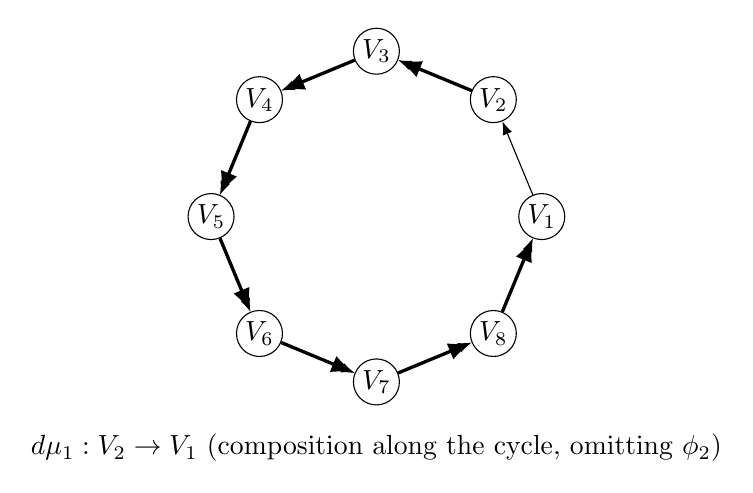
\begin{tikzpicture}[scale=1.05, every node/.style={circle,draw,inner sep=1.2pt}, >=Latex]
        % vertices on a circle
        \def\R{2.0}
        \foreach \i in {1,...,8} {
            \node (v\i) at ({\R*cos(360*(\i-1)/8)},{\R*sin(360*(\i-1)/8)}) {$V_{\i}$};
        }
        % cycle arrows
        \foreach \i [evaluate=\i as \j using {int(mod(\i,8)+1)}] in {1,...,8} {
            \draw[->] (v\i) -- (v\j);
        }
        % highlight a representative path for d\mu_l
        \draw[->,very thick] (v2) -- (v3);
        \draw[->,very thick] (v3) -- (v4);
        \draw[->,very thick] (v4) -- (v5);
        \draw[->,very thick] (v5) -- (v6);
        \draw[->,very thick] (v6) -- (v7);
        \draw[->,very thick] (v7) -- (v8);
        \draw[->,very thick] (v8) -- (v1);
        \node[draw=none,rectangle] at (0,-2.8) {$d\mu_{1}: V_2\to V_1$ (composition along the cycle, omitting $\phi_2$)};
    \end{tikzpicture}
    \caption{The cyclic quiver $C_n$ (illustrated here with $n=8$). The thick arrows indicate the path whose composition gives a typical $d\mu_l$ map along the cycle (example: $d\mu_{2}:V_2\to V_1$).}
\end{figure}

\begin{proposition}[Equivariance of the cyclic composition maps]\label{prop:mu-equivariant}
Let $C_{L+1}$ be the cyclic quiver on vertices $\{0,\ldots,L\}$, let $\mathrm{Rep}_{d}(C_{L+1})$ be its representation space with
$V_l\cong\mathbb{R}^{d_l}$ and. Define the base--change group
\[
G_d:=\prod_{l=0}^{L} \mathrm{GL}(V_l)
\]
acting on $\mathrm{Rep}_{d}(C_{L+1})$ via
\[
(g\cdot \phi)_l := g_l\,\phi_l\,g_{l-1}^{-1},\quad (l=0,\ldots,L), \ \text{mod} \ L+1
\]
Then, for all $g\in G_d$ and all $l=0,\ldots,L$,
\[
d\mu_l(g\cdot \phi) = g_{l-1}\,d\mu_l(\phi)\,g_{l}^{-1}.
\]
\end{proposition}

\begin{proof}
Expand $d\mu_l(g\cdot\phi)$ as a product of the maps $(g\cdot\phi)_i$. Each factor contributes a left multiplication by some $g_{i-1}$ and a right multiplication by $g_{i}^{-1}$, and all intermediate terms cancel by associativity, leaving only $g_{l-1}$ on the left and $g_{l}^{-1}$ on the right.
\end{proof}

\begin{proposition}[Orbit decomposition of $\Gamma_d$]\label{prop:GammaC-orbits}
Let
\[
\Gamma_{d,L+1}:=\Big\{\phi\in \mathrm{Rep}_{d}(C_{L+1})\ \Big|\ d\mu_l(\phi)=0\ \text{for all }l=0,\ldots,L\Big\}.
\]
Then $\Gamma_{d,L+1}$ is $G_d$-invariant. In particular, $\Gamma_{d,L+1}$ decomposes as a disjoint union of $G_d$-orbits:
\[
\Gamma_{d,L+1} = \bigsqcup_{[\phi]\in \Gamma_{d,L+1}/G_d} G_d\cdot \phi .
\]
\end{proposition}

\begin{proof}
By Proposition~\ref{prop:mu-equivariant}, each map $d\mu_l$ is $G_d$-equivariant and hence the vanishing set $d\mu_l^{-1}(0)$ is $G_d$-stable. Intersecting over $l=0,\ldots,L$ shows that $\Gamma_{d,L+1}$ is $G_d$-stable. Any group action partitions a set into disjoint orbits, yielding the stated decomposition.
\end{proof}
\noindent
Informally, we have $\Gamma_{d,L+1}\cong \Rep_d(C_{L+1})/< d\mu_l > $, we will that $\Gamma_{d,L+1}$ is then finite dimensional and we can classify indecomposable using indecomposable representations of Nakayama algebras.
\subsection{Cyclic quiver as a bounded module}
\begin{definition}[Path algebra]
Let $Q$ be a quiver. The \emph{path algebra} $kQ$ is the $k$-vector space with basis given by all directed paths in $Q$ (including the trivial paths $e_i$ of length $0$ at each vertex $i$), with multiplication given by concatenation of composable paths and $0$ otherwise, extended by bilinearity.
\end{definition}

\begin{definition}[Bound quiver algebra associated with $\Gamma_d$]
Let $Q=C_{L+1}$ and for each $l=0,\ldots,L$ let $p_l\in kQ$ be the path
\[
 p_l := a_{l-1}\cdots a_1\,a_{0}\cdots a_{l+1},\ \text{mod } L+1
\]
interpreting empty products as the corresponding trivial path.
Let $I\subset kQ$ be the two-sided ideal generated by $\{p_0,\ldots,p_{L}\}$.
The quotient algebra
\[
A:=kQ/I
\]
is called the \emph{bound quiver algebra} associated with these relations.
\end{definition}

\begin{definition}[Representation of an algebra of dimension $d$]
Let $A$ be a $k$-algebra and let $d=(d_0,\ldots,d_L)$.
A \emph{representation of $A$ of dimension $d$ compatible with the vertices} is a left $A$-module structure on
$V:=\bigoplus_{i=0}^L k^{d_i}$ such that the idempotents $e_i\in kQ\twoheadrightarrow A$ act as the projections onto the $i$-th summand.
We denote the corresponding representation space by $\mathrm{Rep}_d(A)$.
\end{definition}

\begin{proposition}[From quiver representations with relations to $A$-modules]
There is a well-defined map
\[
F:\Gamma_{d,L+1}\to \mathrm{Rep}_d(A)
\]
which sends $\phi\in\Gamma_{d,L+1}$ to the unique $A$-module structure on $V$ for which each arrow $a_i$ acts by the linear map $\phi_i$.
\end{proposition}

\begin{proof}
Given $\phi\in\Gamma_{d,L+1}$, the tuple of linear maps $(\phi_i)_i$ defines a representation of the quiver $Q=C_{L+1}$, hence a left $kQ$-module structure on $V$ by letting a path act by the corresponding composition of arrow maps.
For each $l$, the defining condition $d\mu_l(\phi)=0$ is exactly the statement that the element $p_l\in kQ$ acts as the zero map on $V$.
Since $I$ is the two-sided ideal generated by the $p_l$, every element of $I$ also acts by zero.
Therefore the $kQ$-action factors through the quotient $A=kQ/I$, producing a unique $A$-module structure on $V$ with the required arrow actions.
\end{proof}

\begin{proposition}[From $A$-modules to quiver representations with relations]
There is a well-defined map
\[
G:\mathrm{Rep}_d(A)\to \Gamma_{d,L+1}
\]
which sends an $A$-module structure on $V$ to the induced quiver representation $\phi$ whose arrow maps are the actions of the classes of the arrows $a_i$.
\end{proposition}

\begin{proof}
Let $V$ be a representation in $\mathrm{Rep}_d(A)$.
Composing the action map $A\to \mathrm{End}_k(V)$ with the quotient map $kQ\twoheadrightarrow A$ gives a $kQ$-module structure on $V$.
Restricting the action of each arrow basis element $a_i$ to the appropriate vertex summand yields linear maps $\phi_i:V_{i-1}\to V_{i}$ and hence a point $\phi\in\mathrm{Rep}_d(C_{L+1})$.
Because each $p_l$ maps to zero in $A$, it acts as the zero endomorphism on $V$.
Equivalently, the composed linear map $\mu_l(\phi)$ is zero for every $l$, so $\phi\in\Gamma_{d,L+1}$.
\end{proof}

\begin{proposition}[Correspondence between $\Gamma_{d,L+1}$ and $\mathrm{Rep}_d(A)$]
The maps $F$ and $G$ are mutually inverse bijections. In particular,
\[
\Gamma_{d,L+1} \cong \mathrm{Rep}_d(A),\qquad A=kQ/I.
\]
\end{proposition}

\begin{proof}
Starting from $\phi\in\Gamma_{d,L+1}$, the $A$-module $F(\phi)$ is by construction generated by the same arrow actions as $\phi$, so applying $G$ recovers the same tuple of arrow maps, hence $G(F(\phi))=\phi$.
Conversely, starting from an $A$-module structure on $V$, the map $G$ records the arrow actions and the map $F$ reconstructs the unique $A$-module whose arrow actions agree with those recorded, hence $F(G(V))=V$.
\end{proof}
\begin{lemma}[Finite-dimensionality of $A=kQ/I$]\label{lem:A-finite-dim}
Let $Q=C_{L+1}$ be the oriented cycle on $L+1$ vertices, and let $I\subset kQ$ be the two-sided ideal generated by the paths
$p_0,\dots,p_{L}$, where each $p_l$ is a path of length $L$ (the unique directed path going around the cycle while omitting one arrow).
Then every directed path in $Q$ of length $\ge L +1$ lies in $I$. In particular, $A=kQ/I$ is finite-dimensional.
\end{lemma}

\begin{proof}
Let $q$ be any directed path in $Q$ of length $\ge L+1$. Write $q=b_m b_{m-1}\cdots b_1$ as a concatenation of arrows with $m\ge L+1$.
Consider the contiguous subpath $q':=b_{L}\cdots b_1$ of length $L$. Since $Q$ is an oriented $L+1$-cycle, there is exactly one directed
path of length $L$ from its source to its target, hence $q'$ must coincide with one of the generators $p_l$.
Therefore $q=q''\,p_l$ for some (possibly trivial) path $q''$, so $q\in I$ because $I$ is a two-sided ideal.

Thus all paths of length $\ge L+1$ vanish in $A$, so $A$ is spanned by the residue classes of paths of length $<L+1$, a finite set. Hence $A$ is finite-dimensional.
\end{proof}

\subsection{Bounded modules are Nakayama algebras}
\begin{definition}[$A$-module]
Let $A$ be a (not necessarily commutative) $k$-algebra.
A (left) \emph{$A$-module} is a $k$-vector space $M$ together with a $k$-bilinear map
\[
A\times M\to M,\qquad (a,m)\mapsto a\cdot m,
\]
such that for all $a,b\in A$ and $m\in M$ one has
\[
(ab)\cdot m = a\cdot (b\cdot m),\qquad 1_A\cdot m = m.
\]
A \emph{homomorphism} of $A$-modules is a $k$-linear map commuting with the $A$-action.
\end{definition}

\begin{definition}[Indecomposable module]
An $A$-module $M$ is \emph{indecomposable} if $M\neq 0$ and there do not exist nonzero submodules $M_1,M_2\subset M$ such that
\[
M \cong M_1\oplus M_2.
\]
Equivalently, $M$ is indecomposable if every idempotent endomorphism of $M$ is either $0$ or $\mathrm{id}_M$.
\end{definition}

\begin{definition}[Composition series]
Let $M$ be a finite-dimensional $A$-module.
A \emph{composition series} of $M$ is a finite chain of submodules
\[
0=M_0\subset M_1\subset \cdots \subset M_{\ell}=M
\]
such that each successive quotient $M_i/M_{i-1}$ is \emph{simple}.
The integer $\ell$ is called the \emph{length} of the series.
\end{definition}

\begin{definition}[Projective module]
An $A$-module $P$ is \emph{projective} if for every surjective $A$-module homomorphism $f:M\twoheadrightarrow N$ and every $A$-module homomorphism $g:P\to N$, there exists an $A$-module homomorphism $\tilde g:P\to M$ such that $f\circ \tilde g=g$.
Equivalently, $P$ is projective if the functor $\mathrm{Hom}_A(P,-)$ is exact.
\end{definition}

\begin{definition}[Indecomposable projective module]
A \emph{projective indecomposable} $A$-module is an $A$-module that is both projective and indecomposable.
For a finite-dimensional basic algebra $A$, every indecomposable projective module is of the form $P_i\cong Ae_i$ for a primitive idempotent $e_i\in A$, and every projective module decomposes uniquely as a direct sum of indecomposable projectives.
\end{definition}

\begin{definition}[Uniserial module]
An $A$-module $M$ is \emph{uniserial} if it admits a unique composition series. Equivalently, the set of submodules of $M$ is totally ordered by inclusion.
\end{definition}
\begin{definition}[\textbf{Nakayama algebra}]
Let $A$ be a finite-dimensional $k$-algebra. We say that $A$ is a \emph{Nakayama algebra} if every indecomposable left $A$-module is \emph{uniserial}, i.e.\ it admits a unique composition series.
Equivalently, $A$ is Nakayama if every indecomposable projective left $A$-module is uniserial (and hence every indecomposable injective is uniserial).
\end{definition}

\begin{definition}[Admissible ideal]
Let $Q$ be a finite quiver and let $kQ$ be its path algebra. Write $(kQ)_{\ge m}$ for the $k$-span of all paths of length at least $m$.
A two-sided ideal $I\subset kQ$ is called \emph{admissible} if there exists an integer $m\ge 2$ such that
\[
(kQ)_{\ge m}\subseteq I \subseteq (kQ)_{\ge 2}.
\]
\end{definition}

\begin{definition}[Jacobson radical]
Let $A$ be a (not necessarily commutative) ring. The \emph{Jacobson radical} $J(A)$ is the intersection of all maximal left ideals of $A$.
If $A$ is a finite-dimensional $k$-algebra, then equivalently
\[
J(A)=\bigcap_{S\ \text{simple}} \ker\big(A\to \mathrm{End}_k(S)\big),
\]
i.e.\ $J(A)$ is the largest two-sided ideal that acts by zero on every simple $A$-module.
\end{definition}

\begin{proposition}[\textbf{Bound quiver criterion for Nakayama algebras}]\label{prop:bound-quiver-nakayama}
Let $k$ be a field, let $A \simeq kQ/I$ be a finite-dimensional bound quiver algebra, where $Q$ is a finite quiver and
$I\subset kQ$ is an admissible ideal.
Assume that for every vertex $i\in Q_0$ there is at most one arrow leaving $i$ and at most one arrow entering $i$.
Then $A$ is a Nakayama algebra.

Moreover, if $Q$ is connected and has exactly one arrow leaving and exactly one arrow entering each vertex, then $Q$ is an oriented cycle and $A$ is a \emph{cyclic Nakayama algebra}. If instead $Q$ is connected and has a unique source and a unique sink, then $Q$ is an oriented line and $A$ is a \emph{linear Nakayama algebra}.
\end{proposition}

\begin{proof}
Let $e_i\in kQ\twoheadrightarrow A$ be the primitive idempotent corresponding to a vertex $i\in Q_0$, and consider the indecomposable projective module $P_i := Ae_i$.
As a $k$-vector space, $P_i$ is spanned by residue classes of paths in $Q$ starting at $i$ (modulo the relations in $I$).
Because there is at most one arrow leaving each vertex, for each $\ell\ge 0$ there is \emph{at most one} directed path of length $\ell$ starting at $i$; hence $P_i$ has a basis indexed by (the surviving classes of) these paths.

Let $J\subset A$ denote the Jacobson radical. Since $A\simeq kQ/I$ with $I$ admissible, $J$ is generated (as a two-sided ideal) by the classes of arrows, and one has
\[
J^\ell P_i = J^\ell Ae_i \ \cong\ (J^\ell)e_i,
\]
which is spanned by classes of paths of length $\ge \ell$ starting at $i$.
By the previous paragraph, for each $\ell$ the quotient $J^\ell P_i/J^{\ell+1}P_i$ is either $0$ or a simple module (it is spanned by the class of the unique surviving path of length $\ell$, if it exists).
Therefore the radical filtration
\[
P_i \supset JP_i \supset J^2P_i \supset \cdots
\]
is a chain whose successive quotients are simple (or zero), i.e.\ $P_i$ is uniserial.

Thus every indecomposable projective $P_i$ is uniserial, and hence $A$ is a Nakayama algebra.

For the final statements: if $Q$ is connected and every vertex has exactly one incoming and one outgoing arrow, then the underlying directed graph is a directed cycle. If $Q$ is connected and has a unique source and sink with all other vertices having one incoming and one outgoing arrow, then the directed graph is a directed line. These correspond to cyclic and linear Nakayama algebras respectively.
\end{proof}
\subsection{Cyclic monomial Nakayama algebra with uniform Kupisch series}
Throughout this subsection, let $Q=C_{L+1}$ be the oriented $L+1$-cycle, let $kQ$ be its path algebra, and let
\[
A:=kQ/I
\]
be the bound quiver algebra from Definition~(Bound quiver algebra associated with $\Gamma_{d,L+1}$).

\begin{definition}[Monomial (path) ideal / monomial algebra]
An ideal $I\subset kQ$ is called \emph{monomial} if it is generated (as a two-sided ideal) by paths in $Q$.
A quotient $kQ/I$ with $I$ monomial is called a \emph{monomial algebra}.
\end{definition}

\begin{definition}[Kupisch series]
Let $A$ be a finite-dimensional basic algebra with primitive idempotents $e_0,\ldots,e_{L}$ and indecomposable projectives
$P_i:=Ae_i$.
The \emph{Kupisch series} of $A$ is the $L+1$-tuple
\[
(c_0,\ldots,c_{L}),\qquad c_i:=\ell(P_i),
\]
where $\ell(P_i)$ denotes the composition length of $P_i$.
\end{definition}

\begin{remark}[Loewy length]
For a finite-dimensional algebra $A$ with Jacobson radical $J=J(A)$, the \emph{Loewy length} is the smallest integer $n$ such that $J^n=0$.
\end{remark}

\begin{proposition}[Identification and Kupisch series]
With $Q=C_{L+1}$ and $I=(p_0,\ldots,p_{L})$ as above, the algebra $A=kQ/I$ is a \emph{cyclic monomial Nakayama algebra}.
Moreover its Kupisch series is uniform:
\[
(c_0,\ldots,c_{L})=(L,\ldots,L).
\]
\end{proposition}

\begin{proof}
By construction, the ideal $I$ is generated by the paths $p_0,\ldots,p_{L}$, hence $I$ is monomial and $A$ is a monomial algebra.
By Proposition~\ref{prop:bound-quiver-nakayama}, $A$ is Nakayama; since $Q=C_{L+1}$ is an oriented cycle, $A$ is in fact \emph{cyclic} Nakayama.

Fix a vertex $i$ and consider $P_i=Ae_i$.
Modulo $I$, every path in $Q$ of length $\ge L$ starting at $i$ vanishes, while for each $t=0,1,\ldots,L-1$ there is exactly one directed path of length $t$ starting at $i$.
Therefore $P_i$ has a $k$-basis given by the residue classes of these $L$ paths (length $0$ through $L-1$).

Since $J=J(A)$ is generated by the classes of arrows (as recalled in the proof of Proposition~\ref{prop:bound-quiver-nakayama}), the radical filtration
\[
P_i \supset JP_i \supset J^2P_i \supset \cdots
\]
has successive quotients $J^tP_i/J^{t+1}P_i$ one-dimensional (hence simple) for $t=0,\ldots,L-1$, and zero thereafter.
Thus $\ell(P_i)=L$ for every $i$, which gives the Kupisch series $(L,\ldots,L)$.
\end{proof}

\begin{remark}
Equivalently, $A$ can be viewed as a \emph{truncated cycle algebra}: it is the path algebra of an oriented cycle with all paths of length $\ge L$ killed.
\end{remark}
\subsection{Indecomposable representations of Nakayama algebras}
\begin{definition}[Interval modules]\label{def:interval-modules}
Fix $Q=C_{L+1}$ with vertices $Q_0=\{0,\dots,L\}$ and arrows $a_t:t-1\to t$
for $t=1,\dots,L$, together with $a_0:L\to 0$.
\noindent
The \emph{interval module} $M(i,\ell)$, starting at vertex $i$ and of length $\ell$,
is the representation of $Q$ defined by
\[
M(i,\ell)_j :=
\begin{cases}
k, & j\in\{i,i+1,\dots,i+\ell\}\pmod{L+1},\\
0, & \text{otherwise},
\end{cases}
\]
and for each arrow $a_t:t-1\to t$,
\[
M(i,\ell)_{a_t}:=
\begin{cases}
\mathrm{id}_k, & t\in\{i+1,\dots,i+\ell\}\pmod{L+1},\\
0, & \text{otherwise}.
\end{cases}
\]
\end{definition}
\begin{comment}
\begin{definition}[The uniserial modules $M(i,\ell)$]
Fix $Q=C_{L+1}$ with vertices $Q_0=\{0,\dots,L\}$ and arrows $a_l:l-1\to l$ for $l=0,\dots,L$ with $a_0:L\to 0$.
For $i\in Q_0$ and $0\le \ell\le L$, define a representation $M(i,\ell)$ of $Q$ by
\[
M(i,\ell)_j :=
\begin{cases}
k, & j\in\{i,i+1,\dots,i+\ell\}\ (\mathrm{mod}\ L + 1),\\
0, & \text{otherwise},
\end{cases}
\]
and for each arrow $a_j:j-1\to j$,
\[
M(i,\ell)_{a_j} :=
\begin{cases}
\mathrm{id}_k, & \text{if both source and target are }k,\\
0, & \text{otherwise}.
\end{cases}
\]
\end{definition}
\end{comment}
\begin{lemma}[The relations vanish on $M(i,\ell)$]\label{lem:Miell-well-defined}
Let $Q=C_{L+1}$ and, for each $l\in\{0,\dots,L\}$, let
\[
p_l := a_{l-1}\cdots a_1\, a_{0}a_L\cdots a_{l+1}, \quad \text{mod } L+1
\]
be the oriented path of length $L$ going once around the cycle and omitting $a_l$.
Set $A:=kQ/\langle p_0,\dots,p_{L}\rangle$.
Then, for every $i\in Q_0$ and $0\le \ell\le L$, the representation $M(i,\ell)$ factors through $A$, hence defines a finite-dimensional left $A$-module.
\end{lemma}

\begin{proof}
Fix $i$ and $\ell$. Each path $p_l$ has length $L$.
Since the support of $M(i,\ell)$ contains only $\ell\le L$ consecutive vertices, the corresponding composition along $p_l$ necessarily passes through a vertex where $M(i,\ell)$ is zero.
Therefore $p_l$ acts by the zero map on $M(i,\ell)$ for every $l$, so all generators of the ideal $\langle p_0,\dots,p_{L}\rangle$ act trivially.
Hence the $kQ$-action factors through $A$.
\end{proof}
\begin{lemma}[Indecomposability of $M(i,\ell)$]\label{lem:Miell-uniserial}
For every interval module $M(i,\ell)$, the $A$-module $M(i,\ell)$ is uniserial, and in particular indecomposable.
\end{lemma}

\begin{proof}
Let $N\subseteq M(i,\ell)$ be a nonzero submodule. Since $N\neq 0$, there exists a vertex
$t$ such that $N_t\neq 0$. As $N_t\subseteq M(i,\ell)_t$ and each nonzero vertex space
of $M(i,\ell)$ is one-dimensional, we must have
\[
N_t=M(i,\ell)_t\cong k.
\]
\noindent
Write the support of $M(i,\ell)$ as the ordered interval
\[
i,\, i+1,\, \dots,\, i+\ell
\]
(along the chosen orientation, modulo $L+1$), and choose $t$ minimal such that
$N_t\neq 0$. Then $N_s=0$ for all vertices $s$ preceding $t$ in this interval.
\noindent
Now for each vertex $r$ with
\[
t\le r\le i+\ell-1,
\]
the arrow
\[
a_{r+1}\colon r\to r+1
\]
acts as the identity on $M(i,\ell)$. Since $N$ is a subrepresentation and
$N_r=M(i,\ell)_r\cong k$, its image under $a_{r+1}$ is nonzero, hence
\[
N_{r+1}=M(i,\ell)_{r+1}.
\]
By induction we obtain
\[
N_r=M(i,\ell)_r
\qquad\text{for all } r=t,t+1,\dots,i+\ell,
\]
and $N_r=0$ at all earlier vertices in the support and outside the support.
\noindent
Therefore every nonzero submodule $N$ is exactly a terminal interval submodule,
namely
\[
N \cong M\bigl(t,\, i+\ell-t\bigr)
\]
(with indices read modulo $L+1$). Hence the nonzero submodules of $M(i,\ell)$
are precisely the terminal subintervals of the support, and these are totally
ordered by inclusion. Explicitly, they form the chain
\[
0
\subset
M(i+\ell,0)
\subset
M(i+\ell-1,1)
\subset
M(i+\ell-2,2)
\subset
\cdots
\subset
M(i,\ell).
\]
\noindent
Here $M(i+\ell-r,r)$ is the submodule supported on the vertices
\[
i+\ell-r,\; i+\ell-r+1,\; \dots,\; i+\ell,
\]
that is, the terminal interval of length $r$ inside the support
\[
i,\; i+1,\; \dots,\; i+\ell.
\]
Thus $M(i,\ell)$ is uniserial.
\noindent
Finally, every uniserial module is indecomposable: if
\[
M(i,\ell)=U\oplus V
\]
with $U,V\neq 0$, then $U$ and $V$ are two nonzero submodules neither of which
contains the other, contradicting the fact that the submodules are totally
ordered. Hence $M(i,\ell)$ is indecomposable.
\end{proof}

\begin{lemma}[Endomorphisms of $M(i,\ell)$]\label{lem:Miell-end}
For every interval module $M(i,\ell)$ one has
\[
\End_A(M(i,\ell))\cong k.
\]
\end{lemma}

\begin{proof}
Let $f\in \End_A(M(i,\ell))$.
At each vertex $t$ in the support $[i\rightsquigarrow i+\ell]$, the map $f_t$
is multiplication by some scalar $\lambda_t\in k$.
\noindent
For each arrow inside the support, the arrow map is $\mathrm{id}_k$, so
commutativity of
\[
f_{t+1}\circ M(i,\ell)_{a_{t+1}} = M(i,\ell)_{a_{t+1}}\circ f_t
\]
implies $\lambda_{t+1}=\lambda_t$. Hence all $\lambda_t$ coincide, and
therefore $f=\lambda\,\mathrm{id}$ for some $\lambda\in k$.
\end{proof}§

\begin{lemma}[Projective truncations realize interval modules]
Let $P(i):=Ae_i$ be the indecomposable projective at vertex $i$ and let $J:=J(A)$.
Then, for every $i\in Q_0$ and every $0\le \ell\le L-1$, there is an isomorphism of $A$-modules
\[
P(i)/J^{\ell+1}P(i)\cong M(i,\ell),
\]
where indices are taken modulo $L+1$.
\end{lemma}

\begin{proof}
By Proposition~\ref{prop:bound-quiver-nakayama} and the previous subsection,
$A$ is a cyclic Nakayama algebra with uniform Kupisch series $(L,\ldots,L)$.
In particular, $P(i)$ is uniserial of length $L$, and $J^tP(i)$ is spanned
by residue classes of paths of length $\ge t$ starting at $i$.
\noindent
Thus $P(i)/J^{\ell+1}P(i)$ has a basis given by the residue classes of the
unique paths of lengths
\[
0,1,\dots,\ell
\]
starting at $i$.
\noindent
Under the induced quiver description, this quotient has one-dimensional
spaces on the vertices
\[
i,i+1,\dots,i+\ell \pmod{L+1},
\]
and identity maps along arrows inside the support. This is precisely the
interval module $M(i,\ell)$.
\end{proof}
\begin{proposition}[Indecomposables of the cyclic truncated Nakayama algebra]\label{prop:indecomp-cyclic-nakayama}
Let $A=kQ/I$ be the cyclic truncated Nakayama algebra associated with $Q=C_{L+1}$,
where $I$ is generated by the paths $p_0,\dots,p_L$ of length $L$.
Then every finite-dimensional indecomposable $A$-module is isomorphic to an
interval module
\[
M(i,\ell)
\]
for a unique pair $(i,\ell)$ such that
\[
i\in Q_0, \qquad 0\le \ell\le L-1 .
\]
\noindent
Equivalently, every indecomposable $A$-module is of the form
\[
P(i)/J^{\ell+1}P(i)
\]
for a unique pair $(i,\ell)$ with
\[
0 \le \ell \le L-1 .
\]
\noindent
In particular, $A$ has exactly
\[
L(L+1)
\]
indecomposable modules up to isomorphism.
\end{proposition}

\begin{proof}
By Lemma~\ref{lem:Miell-well-defined}, each $M(i,\ell)$ is a well-defined
finite-dimensional $A$-module, and by Lemma~\ref{lem:Miell-uniserial}
it is indecomposable.
\noindent
Conversely, since $A$ is Nakayama
(Proposition~\ref{prop:bound-quiver-nakayama}),
every indecomposable $A$-module is uniserial and hence a quotient of a unique
indecomposable projective $P(i)=Ae_i$.
\noindent
Because all paths of length $L$ vanish in $A$, the indecomposable projective
$P(i)$ has composition length $L$. Hence every indecomposable quotient of
$P(i)$ is of the form
\[
P(i)/J^{\ell+1}P(i)
\]
for some $0\le \ell \le L-1$.
\noindent
By Lemma~\ref{lem:Miell-uniserial}, this module is isomorphic to
\[
M(i,\ell).
\]
\noindent
Uniqueness follows because the top simple module determines $i$ and the
length determines $\ell$.
\noindent
For each $i\in Q_0$ there are $L$ possible values of $\ell$, namely
$0,\dots,L-1$. Since $|Q_0|=L+1$, this yields a total of
\[
L(L+1)
\]
indecomposable modules up to isomorphism.
\end{proof}
\noindent
More details about Nakayama algebras and their representations can be found in the following lecture notes:
\href{https://www.math.uni-bielefeld.de/~wcrawley/1920noncommalg2/NA2.pdf}{Noncommutative Algebra 2: Representations of finite-dimensional algebras} in particular theorem and corollary section 1.6.
We have a Krull--Schmidt theorem for these Nakayama algebras.
\begin{proposition}[Krull--Schmidt for the cyclic truncated Nakayama algebra]\label{prop:KS-cyclic-truncated-nakayama}
Let $A=kQ/I$ be the cyclic truncated Nakayama algebra, where $Q=C_{L+1}$ is the oriented $(L+1)$-cycle and $I$ is the ideal generated by the paths $p_0,\dots,p_{L}$ of length $L$ (equivalently, all paths of length $\ge L$ vanish in $A$).
Let $\mathrm{mod}\text{-}A$ denote the category of finite-dimensional left $A$-modules.
\noindent
Then every $M\in \mathrm{mod}\text{-}A$ admits a decomposition as a finite direct sum of indecomposable $A$-modules.
Moreover, this decomposition is unique up to reordering and isomorphism of the indecomposable summands.
\noindent
Equivalently, using the explicit indecomposables $M(i,\ell)$ from proposition~\ref{prop:indecomp-cyclic-nakayama}, there exist uniquely determined multiplicities
$m_{i,\ell}\in\mathbb{Z}_{\ge 0}$ such that
\[
M \ \cong\ \bigoplus_{i=0}^{L} \ \bigoplus_{\ell=0}^{L-1} \ M(i,\ell)^{\oplus m_{i,\ell}}.
\]
\end{proposition}

\begin{proof}[Proof sketch]
Since $A$ is finite-dimensional over $k$, it is left artinian (and left noetherian), hence every object of $\mathrm{mod}\text{-}A$ has finite length.
In particular, $\mathrm{mod}\text{-}A$ is a Krull--Schmidt category: every object decomposes as a finite direct sum of indecomposables, and such a decomposition is unique up to permutation and isomorphism.
\noindent
Concretely, existence follows by choosing a nonzero module $M$ and repeatedly splitting off a nontrivial direct summand until all summands are indecomposable; the process terminates because $M$ has finite length.
Uniqueness follows because each indecomposable has a local endomorphism ring (for example, by Lemma~\ref{lem:Miell-end} in the explicit classification), and the classical Krull--Schmidt--Azumaya argument applies.
\noindent
Finally, Proposition~\ref{prop:indecomp-cyclic-nakayama} classifies the indecomposables as the modules $M(i,\ell)$ with $0\le \ell\le L-1$, so any Krull--Schmidt decomposition can be rewritten uniquely in the stated multiplicity form.
\end{proof}
\noindent
\textbf{Note}: This latter proposition enables to parameterize the orbits of $\Gamma$ with the indecomposables representations.
\begin{remark}[On the choice of base field]
Although we work over the field $\mathbb{R}$, the combinatorial
description of the strata of $\Gamma$ does not depend on whether the
base field is $\mathbb{R}$ or $\mathbb{C}$.

Indeed, the cyclic vanishing relations identify the relevant
representation space with the representation space of the
finite-dimensional algebra $A = kQ/I$, where $Q$ is the cyclic quiver
and $I$ is generated by the length-$L$ cyclic paths. As shown in
Section~4, $A$ is a cyclic Nakayama algebra. Its indecomposable modules
are explicitly given by the interval modules $M(i,\ell)$, whose
structure maps are either the identity or the zero map. In particular,
these indecomposable modules are defined over any base field and do not
involve additional scalar parameters.

Since $A$ is finite dimensional, the Krull--Schmidt theorem applies,
and every $A$--module admits a unique decomposition into indecomposable
modules $M(i,\ell)$. Consequently the multiplicity data indexing the
strata of $\Gamma$ are independent of whether the base field is
$\mathbb{R}$ or $\mathbb{C}$. 
\end{remark}
\begin{comment}
\paragraph{Orbits, isomorphism classes, and multiplicity patterns.}
Fix a finite-dimensional $k$-algebra $A$ and a dimension vector $d=(d_0,\dots,d_{L})$.
Recall that
\[
\mathrm{Rep}_d(A)
=\Big\{\text{left $A$-module structures on }V=\bigoplus_{i=0}^{L} k^{d_i}\text{ such that each idempotent $e_i$ acts as the projection onto }k^{d_i}\Big\}.
\]
Let
\[
G_d:=\prod_{i=0}^{L} \mathrm{GL}(k^{d_i})
\]
act on $\mathrm{Rep}_d(A)$ by \emph{change of bases at the vertices} (equivalently, by transport of structure):
for $g=(g_0,\dots,g_L)\in G_d$ and a module structure $\rho:A\to \mathrm{End}_k(V)$, define a new module
structure $g\cdot \rho$ by
\[
(g\cdot \rho)(a)\;:=\; g\,\rho(a)\,g^{-1},\qquad g:=\bigoplus_{i=1}^n g_i\in \mathrm{GL}(V).
\]
When $A\simeq kQ/I$ is presented as a bound quiver algebra, this action is equivalently given on arrow
maps by $(g\cdot \phi)_a=g_{t(a)}\,\phi_a\,g_{s(a)}^{-1}$.
Then two points $\rho,\rho'\in \mathrm{Rep}_d(A)$ lie in the same $G_d$-orbit if and only if the corresponding
$A$-modules $(V,\rho)$ and $(V,\rho')$ are isomorphic in $\mathrm{mod}\text{-}A$.
Consequently, there is a canonical bijection
\[
\big(G_d\backslash \mathrm{Rep}_d(A)\big)\ \cong\ \Big\{\text{isomorphism classes of $A$-modules $M$ with $\dim(e_iM)=d_i$ for all $i$}\Big\}.
\]

Now specialize to the cyclic truncated Nakayama algebra $A=kQ/I$ considered above.
Its indecomposable modules are the uniserials $M(i,\ell)$ with $i\in\{0,\dots,L\}$ (indices taken modulo $L+1$) and $1\le \ell\le L$
(Proposition~\ref{prop:indecomp-cyclic-nakayama}).
By the Krull--Schmidt theorem (Proposition~\ref{prop:KS-cyclic-truncated-nakayama}), every finite-dimensional
$A$-module $M$ admits a decomposition
\[
M\ \simeq\ \bigoplus_{i=0}^{L}\ \bigoplus_{\ell=1}^{L} M(i,\ell)^{\oplus m_{i,\ell}},
\qquad m_{i,\ell}\in\mathbb{Z}_{\ge 0},
\]
and this decomposition is unique up to permutation of summands.
The multiplicities $(m_{i,\ell})$ determine (and are constrained by) the dimension vector $d$ via the \emph{covering equations}
\begin{equation}\label{eq:cyclic-multiplicity-constraints}
d_k \;=\; \sum_{i=0}^{L}\ \sum_{\ell=1}^{L} m_{i,\ell}\,\mathbf{1}\!\left\{k\in\{i,i+1,\dots,i+\ell-1\}\ (\mathrm{mod}\ L+1)\right\},
\qquad k=0,\dots,L,
\end{equation}
since $M(i,\ell)$ contributes a one-dimensional space at vertex $k$ exactly when $k$ lies in its cyclic
support interval of length $\ell$ starting at $i$.
Define the set of \emph{multiplicity patterns}
\[
M_d^{+}(A)
:=\left\{(m_{i,\ell})\in \mathbb{Z}_{\ge 0}^{L(L+1)}\ \middle|\ \text{\eqref{eq:cyclic-multiplicity-constraints} holds for all }k\right\}.
\]
Then the above discussion yields a concrete parametrization of orbits:
every $G_d$-orbit in $\mathrm{Rep}_d(A)$ corresponds to a unique isomorphism class in $\mathrm{mod}\text{-}A$,
and hence to a unique multiplicity pattern $(m_{i,\ell})\in M_d^{+}(A)$ via its Krull--Schmidt decomposition.
In other words, we obtain canonical bijections
\[
G_d\backslash \mathrm{Rep}_d(A)
\ \cong\
\Big\{\text{isomorphism classes in $\mathrm{mod}\text{-}A$ with dimension vector $d$}\Big\}
\ \cong\
M_d^{+}(A),
\]
where the last map sends an $A$-module to the multiplicities of the indecomposables $M(i,\ell)$ in its Krull--Schmidt decomposition.
\end{comment}
\begin{definition}
    Consider a $A$ module $M$ and its Krull-Schmidt decomposition into $M(i,\ell)$ for $i\in\{0,\dots,L\}$ and $\ell\in\{0,\dots,L-1\}$. For each vertex $k$ the dimension $d_k$ of the representation $M$ at vertex $k$ satisfies the dimension constraint:
\[d_k \;=\;
\sum_{i=0}^{L}\sum_{\ell=0}^{L-1}
m_{i,\ell}\,\mathbf{1}\!\left\{
k \in \{i,i+1,\dots,i+\ell\} \ (\mathrm{mod}\ L+1)
\right\}\quad k=0,\dots,L\]
Define the set of \emph{multiplicity patterns} as
\[\mathcal M_d^+ := \left\{(m_{i,\ell})\in \mathbb{Z}_{\ge 0}^{L(L+1)}\middle|\ \text{the above dimension constraints hold for all }k\right\}.\]
\end{definition}
\begin{definition}
    For each $m \in \mathcal M_d^+(A)$, define the stratum
\[
\mathcal{O}_m
:=
\left\{
\phi \in \Gamma_{d,L+1}
\;\middle|\;
M(\phi) \cong
\bigoplus_{i,\ell} M(i,\ell)^{\oplus m_{i,\ell}}
\right\},
\]
$\mathcal{O}_m$ is a single $G_d$-orbit and $\phi_m$ is a particular representative in this orbit. 
\end{definition}
\begin{proposition}[Orbit stratification of $\Gamma_{d,L+1}$ by indecomposable Nakayama modules]
\label{prop:Gamma_orbit_stratification}

Fix $L \ge 1$ and let $Q = C_{L+1}$ be the oriented cyclic quiver on vertices
$\{0,\dots,L\}$.  
Let $A := kQ/I$ be the bound quiver algebra, where $I$ is the ideal generated by the length-$L$
paths $p_0,\dots,p_{L}$ obtained by going once around the cycle and omitting one arrow.
Let $d=(d_0,\dots,d_L)$ be a dimension vector. 
The variety $\Gamma_{d,L+1}$ decomposes as a disjoint union of these orbits:
\[
\Gamma_{d,L+1}
\;=\;
\bigsqcup_{m \in \mathcal M_d^+(A)} \mathcal{O}_m
\;=\;
\bigsqcup_{m \in \mathcal M_d^+(A)} G_d \cdot \phi_m,
\]
where $\phi_m$ is any representative whose associated $A$-module has multiplicity pattern $m$.
\noindent
In particular, the $G_d$-orbits in $\Gamma_{d,L+1}$ are parameterized by the
multiplicity data of indecomposable $A$-modules, i.e.\ by the set
$\mathcal M_d^+(A)$.
\end{proposition}
\section{Stratification of vanishing cyclic conditions with fixed closing map}
While the indecomposable representation of $\Gamma_{d,\sigma}$ are parameterized by the $M(i,\ell)$ we are actually interested in stratifying:
\begin{equation*}
    \Gamma_{d,\sigma} := \left\{(\phi_0,\ldots,\phi_{L})\in \mathrm{Rep}_d(C_{L+1})\;\middle|\; \phi_{l-1}\cdots\phi_1\,\phi_{0}\,\phi_L\cdots\phi_{l+1} = 0,\; \phi_{0}=\sigma\right\}.
\end{equation*}
where the map $\sigma\in \mathrm{Hom}(V_L,V_0)$ is fixed (for a DLN it is the map $\Sigma_{XY}U_Q$).
The map
\begin{equation*}
    d\mu_{l,\sigma} := \phi_{l-1}\cdots\phi_1\,\sigma\,\phi_L\cdots\phi_{l+1}
\end{equation*}
is no longer $G_d$-equivariant.

\begin{definition}[Stabilizer group of the fixed arrow]\label{def:stabilizer-sigma}
Let $\sigma\in\mathrm{Hom}(V_L,V_0)$ be fixed. Define
\[
\mathrm{Stab}(\sigma):=\{(g_0,g_L)\in \mathrm{GL}(V_0)\times \mathrm{GL}(V_L)\mid g_0\,\sigma\,g_L^{-1}=\sigma\},
\]
and the corresponding subgroup of the base--change group
\[
G_\sigma:=\{g=(g_0,\ldots,g_L)\in \prod_{l=0}^L\mathrm{GL}(V_l)\mid (g_0,g_L)\in \mathrm{Stab}(\sigma)\}.
\]
\end{definition}

\begin{proposition}[$G_\sigma$-equivariance of the cyclic composition maps]\label{prop:mu-sigma-equivariant}
Fix $\sigma\in\mathrm{Hom}(V_L,V_0)$ and consider the representation space with $\phi_{0}=\sigma$.
For $\phi=(\sigma,\phi_1,\ldots,\phi_L)$ and each $l=0,\ldots,L$, define
\[
d\mu_{l,\sigma}(\phi):=\phi_{l-1}\cdots \phi_1\,\sigma\,\phi_L\cdots \phi_{l+1}\in\mathrm{Hom}(V_{l},V_{l-1}),
\]
with the convention that an empty product is the identity.
Then, for all $g\in G_\sigma$ and all $l$,
\[
d\mu_{l,\sigma}(g\cdot \phi)= g_l\,d\mu_{l,\sigma}(\phi)\,g_{l+1}^{-1}.
\]
In particular, the subset $\Gamma_{d,\sigma}=\bigcap_{l=0}^L d\mu_{l,\sigma}^{-1}(0)$ is $G_\sigma$-invariant.
\end{proposition}

\begin{proof}
Expand $d\mu_{l,\sigma}(g\cdot\phi)$ as a product of the maps $(g\cdot\phi)_i$.
All intermediate base-change factors cancel. The only remaining factors are $g_l$ on the left and
$g_{l+1}^{-1}$ on the right. The middle arrow is $(g\cdot\phi)_{0}=g_0\sigma g_L^{-1}$, which equals
$\sigma$ because $g\in G_\sigma$. 
\end{proof}
\noindent
For all modules in $\Gamma_{d,\sigma}$ Krull-Schmidt applies (as a category of $A$-modules where $A$ is finite dimensional). We want to parameterize the orbits of $\Gamma_{d,\sigma}$ under the action of $G_\sigma$ to obtain a combinatorial description of the saddle points.
\begin{lemma}[Intersection of a $G_d$--orbit with a fixed--arrow fiber]
\label{lem:orbit_fiber_intersection}
Let $L\ge 2$ and let $V_0,\dots,V_L$ be finite--dimensional vector spaces over a field $\Bbbk$.  
Let $\mathcal O\subset \Gamma_{d,L+1}$ be a single $G_d$--orbit.  
Then either $\mathcal O\cap\Gamma_{d,\sigma}=\varnothing$, or else for every
$x\in\mathcal O\cap\Gamma_{d,\sigma}$ one has
\[
\mathcal O_{\sigma}:=\mathcal O\cap\Gamma_{d,\sigma} \;=\; G_\sigma\cdot x .
\]
In particular, whenever $\mathcal O\cap\Gamma_{d,\sigma}\neq\varnothing$, this
intersection consists of a single $G_\sigma$--orbit.
\end{lemma}
\noindent
We prove this lemma in the appendix \ref{proof-lem:orbit_fiber_intersection}.
\begin{proposition}[Rank label for Nakayama orbits and the fiber non-emptiness criterion over $\mathbb{R}$]
\label{prop:rank_label_and_nonemptiness_real}
Consider the morphism:
\[
F:\Gamma_d \longrightarrow \Hom_{\mathbb{R}}(V_L,V_0)
\]
satisfying the equivariance identity
\begin{equation}
\label{eq:equivariance_F}
F\!\big((g_0,\dots,g_L)\cdot x\big)=g_0\,F(x)\,g_L^{-1}
\qquad\text{for all } (g_0,\dots,g_L)\in G_d,\; x\in \Gamma_d .
\end{equation}
\medskip
\noindent
Consider a stratification of $\Gamma_{d,\sigma}$ into $G_d$--orbits indexed by a parameter set $\Lambda$,
\[
\Gamma_{d,\sigma} \;=\; \bigsqcup_{\lambda\in\Lambda}\, \mathcal O_\lambda,
\]
where $\mathcal O_\lambda$ denotes the $G_d$--orbit corresponding to $\lambda$ (in the context of this paper, $\lambda$ corresponds to the Krull--Schmidt multiplicities of the Nakayama indecomposables).  
For each $\lambda\in\Lambda$, define the integer
\begin{equation}
\label{eq:def_r_lambda}
r(\lambda) \;:=\; \mathrm{rank}\big(F(x)\big)\quad \text{for any } x\in \mathcal O_\lambda.
\end{equation}

\medskip
\noindent
Then the following statements hold.

\begin{enumerate}
\item[(i)] The integer $r(\lambda)$ in \eqref{eq:def_r_lambda} is well-defined, i.e.\ it does not depend on the choice of $x\in \mathcal O_\lambda$.
\item[(ii)] Fix $\sigma\in W$ and define the fiber $\Gamma_\sigma:=F^{-1}(\sigma)$. Then for every $\lambda\in\Lambda$,
\begin{equation}
\label{eq:nonemptiness}
\mathcal O_\lambda\cap \Gamma_\sigma \neq \varnothing
\qquad\Longleftrightarrow\qquad
r(\lambda)=\mathrm{rank}(\sigma).
\end{equation}
\end{enumerate}
\end{proposition}
\noindent
The proof of this proposition is given in the appendix \ref{proof:rank_label_and_nonemptiness_real}.
\begin{comment}
\begin{proposition}[Rank stratification of $\Gamma_{XY}$ by Nakayama types]
\label{prop:GammaXY_orbit_decomposition}
Let $d=(d_1,\dots,d_L)$ be a dimension vector and let
\[
\Gamma_d \subset \Rep_d(C_{L+1})
\]
be the variety defined in Section~\S9.
Recall that $\Gamma_d$ admits a decomposition into $G_d$--orbits indexed by
\[
\mathcal M_d^+ \;=\; \left\{ (m_{i,\ell}) \;\middle|\; 
\sum_{i,\ell} m_{i,\ell}\,\underline{\dim} M(i,\ell)=d
\right\},
\]
where $M(i,\ell)$ are the indecomposable modules of the cyclic Nakayama algebra
and $(m_{i,\ell})$ records their multiplicities.
For $\mathbf m=(m_{i,\ell})\in\mathcal M_d^+$, denote by
$\mathcal O_{\mathbf m}\subset\Gamma_d$ the corresponding $G_d$--orbit.

Let
\[
F:\Gamma_d\longrightarrow \Hom(V_L,V_1),
\qquad
F(\phi)=\phi_{L+1},
\]
and fix a linear map $\sigma\in\Hom(V_L,V_1)$.
Define
\[
\Gamma_{XY}:=\Gamma_\sigma:=F^{-1}(\sigma),
\qquad
G_\sigma:=\{g\in G_d:\ g_1\sigma g_L^{-1}=\sigma\}.
\]

For $\mathbf m\in\mathcal M_d^+$, define the integer
\[
r(\mathbf m)\;:=\;\mathrm{rank}\big(F(\phi)\big)
\quad\text{for any }\phi\in\mathcal O_{\mathbf m}.
\]
Then:

\begin{enumerate}
\item[(i)] The integer $r(\mathbf m)$ is well-defined (independent of the choice of
$\phi\in\mathcal O_{\mathbf m}$).

\item[(ii)] For every $\mathbf m\in\mathcal M_d^+$,
\[
\mathcal O_{\mathbf m}\cap \Gamma_{XY}\neq\varnothing
\quad\Longleftrightarrow\quad
r(\mathbf m)=\mathrm{rank}(\sigma).
\]

\item[(iii)] If $\mathcal O_{\mathbf m}\cap \Gamma_{XY}\neq\varnothing$, then
\[
\mathcal O_{\mathbf m}\cap \Gamma_{XY}
\]
is a single $G_\sigma$--orbit.

\item[(iv)] Consequently, $\Gamma_{XY}$ admits the disjoint decomposition
\[
\Gamma_{XY}
\;=\;
\bigsqcup_{\mathbf m\in\mathcal M_d^+ \;:\; r(\mathbf m)=\mathrm{rank}(\sigma)}
\big(\mathcal O_{\mathbf m}\cap \Gamma_{XY}\big),
\]
and each stratum in this decomposition is a single $G_\sigma$--orbit.
\end{enumerate}
\end{proposition}
\end{comment}
\begin{definition}
    Fix $L\ge 2$ and a dimension vector $d=(d_0,\dots,d_L)$.
Recall that
$\Gamma_{d,L+1}$ decomposes into $G_d$--orbits indexed by $\mathcal M_d^+$, i.e.\ for each
\[
\mathbf m=(m_{i,\ell})\in \mathcal M_d^+
\]
there is a corresponding $G_d$--orbit $\mathcal O_{\mathbf m}\subset \Gamma_{d,L+1}$ such that
every $\phi\in \mathcal O_{\mathbf m}$ has associated Nakayama module
\[
M(\phi)\;\cong\;\bigoplus_{i,\ell} M(i,\ell)^{\oplus m_{i,\ell}}
\]
(up to isomorphism), where $M(i,\ell)$ denote the indecomposable modules of the cyclic Nakayama algebra.
For $\mathbf m\in\mathcal M_d^+$ define
\[
r(\mathbf m)\;:=\;\rank(F(\phi))\qquad\text{for any }\phi\in\mathcal O_{\mathbf m},
\]
which is well-defined by Proposition~\ref{prop:rank_label_and_nonemptiness_real}.
\end{definition}
\begin{definition}
    For an indecomposable $M(i,\ell)$, define its \emph{support interval} to be the cyclic set of vertices
\[
\Supp(i,\ell)\;:=\;\{\,i,\; i+1,\; \dots,\; i+\ell\,\}\subset \mathbb{Z}/(L+1)\mathbb{Z},
\]
where addition is taken modulo $L+1$ and we identify vertices with their residue classes.
Say that $M(i,\ell)$ is \emph{$(L\to 0)$--active} if the arrow $L\to 0$ acts nontrivially on $M(i,\ell)$,
i.e.\ if the closing map
\[
M(i,\ell)(L)\longrightarrow M(i,\ell)(0)
\]
induced by the quiver arrow $L\to 0$ is nonzero.
Define the indicator
\[
\epsilon(i,\ell)\;:=\;
\begin{cases}
1, & \text{if $M(i,\ell)$ is $(L\to 0)$--active},\\
0, & \text{otherwise}.
\end{cases}
\]
\end{definition}
\begin{proposition}[Rank formula for the closing arrow in terms of Nakayama multiplicities]
\label{prop:rank_formula_eps}
For every $\mathbf m=(m_{i,\ell})\in \mathcal M_d^+$ one has the formula
\begin{equation}
\label{eq:rank_formula_eps}
r(\mathbf m)\;=\;\sum_{i=0}^L\sum_{\ell=1}^L\epsilon(i,\ell)\,m_{i,\ell}.
\end{equation}
\end{proposition}
\noindent
The proof of that proposition is given in the appendix \ref{proof:rank_formula_eps}.
\begin{corollary}[Orbit decomposition of $\Gamma_{XY}$ indexed by $\mathcal M_d^+$]
\label{cor:GammaXY_decomposition_by_Mdplus}
Recall $\Gamma_{d,XY}=\Gamma_{d,\sigma}:=F^{-1}(\sigma)$,
the $G_d$--orbits in $\Gamma_d$ are denoted $\mathcal O_{\mathbf m}$ for $\mathbf m\in\mathcal M_d^+$,
and $G_\sigma:=\{g\in G_d:\ g_0\sigma g_L^{-1}=\sigma\}$. Consider the orbit:
\begin{equation*}
    \mathcal O_{\mathbf m, \sigma} := \mathcal O_{\mathbf m}\cap \Gamma_{d,XY}.
\end{equation*}
Then $\Gamma_{d,XY}$ decomposes as a disjoint union of $G_\sigma$--orbits indexed by those
$\mathbf m\in\mathcal M_d^+$ satisfying the rank constraint:
\[
\Gamma_{d,XY}
\;=\;
\bigsqcup_{\mathbf m\in\mathcal M_d^+\;:\; r(\mathbf m)=\rank(\sigma)}
 \mathcal O_{\mathbf m, \sigma},
\]
and for each such $\mathbf m$ the set $ \mathcal O_{\mathbf m, \sigma}$ is a single $G_\sigma$--orbit.
\noindent
Moreover, for $\mathbf m=(m_{i,\ell})\in\mathcal M_d^+$ the integer $r(\mathbf m)$ is given by the explicit formula
\[
r(\mathbf m)\;=\;\sum_{i,\ell}\epsilon(i,\ell)\,m_{i,\ell},
\]
where $\epsilon(i,\ell)\in\{0,1\}$ is the $(L\to 0)$--activity indicator of the indecomposable $M(i,\ell)$
as in Proposition~\ref{prop:rank_formula_eps}.
\end{corollary}

\begin{proof}
Fix $\sigma\in\Hom(V_L,V_0)$ and recall $\Gamma_{d,XY}=\Gamma_{d,\sigma}$. First, since $\Gamma_{d,L+1}=\bigsqcup_{\mathbf m\in\mathcal M_d^+}\mathcal O_{\mathbf m}$ is a disjoint union,
intersecting with $\Gamma_\sigma$ gives the disjoint union
\[
\Gamma_{d,\sigma}
\;=\;
\Gamma_{d,\sigma}\cap \Gamma_{d,L+1}
\;=\;
\Gamma_{d,\sigma}\cap \Gamma_{d,L+1}
\;=\;
\Gamma_{d,\sigma} \cap \left(\bigsqcup_{\mathbf m\in\mathcal M_d^+}\mathcal O_{\mathbf m}\right)
\;=\;
\bigsqcup_{\mathbf m\in\mathcal M_d^+}\mathcal O_{\mathbf m, \sigma}.
\]
By Proposition~\ref{prop:rank_label_and_nonemptiness_real}, for a given $\mathbf m$ the intersection
$\mathcal O_{\mathbf m}\cap \Gamma_{d,\sigma}$ is nonempty if and only if
$r(\mathbf m)=\rank(\sigma)$. Therefore all terms with $r(\mathbf m)\neq\rank(\sigma)$ vanish,
and we obtain
\[
\Gamma_{d,\sigma}
\;=\;
\bigsqcup_{\mathbf m\in\mathcal M_d^+\;:\; r(\mathbf m)=\rank(\sigma)}
\mathcal O_{\mathbf m, \sigma}.
\]
Again by Proposition~\ref{prop:rank_label_and_nonemptiness_real}, whenever the intersection is nonempty,
$\mathcal O_{\mathbf m}\cap \Gamma_{d,\sigma}$ is a single $G_\sigma$--orbit. This proves the stated orbit
decomposition.
\end{proof}
\begin{remark}[Parametrization of $G_\sigma$--orbits in $\Gamma_{XY}$]
\label{rem:GammaXY_Gsigma_orbits}
The previous corollary can be equivalently phrased as follows.
The $G_\sigma$--orbits in $\Gamma_{d,XY}$ are in bijection with the subset
\[
\left\{\mathbf m\in \mathcal M_d^+ \;\middle|\; r(\mathbf m)=\rank(\sigma)\right\},
\]
via the correspondence
\[
\mathbf m
\;\longmapsto\;
\mathcal O_{\mathbf m}\cap \Gamma_{d,\sigma}.
\]
In particular, $\Gamma_{d,XY}$ decomposes as a disjoint union of $G_\sigma$--orbits indexed by
Nakayama indecomposable multiplicity data satisfying the rank constraint $r(\mathbf m)=\rank(\sigma)$.
\end{remark}
%%%%%%%%%%%%%%%%%%%%%%%%%%%%%%%%%%%%%%%%%%%%%%%%%%%%%%%%%%%%%%
\subsection{Cyclic rank patterns and multiplicities}

\paragraph{Convention on interval modules.}
From this subsection onward we index indecomposable interval modules by
their \emph{endpoints}. Thus $M(k,\ell)$ denotes the indecomposable
representation supported on the cyclic interval
\[
[k\leadsto \ell],
\]
with length $\delta(k,\ell)\le L$. In particular the representation has
one--dimensional vector spaces along the vertices
$k,k+1,\dots,\ell$ and identity maps along the arrows in this segment,
and zero elsewhere. This convention differs from the length indexing
used in previous sections and will be used from now on.

\paragraph{Cyclic intervals.}
For $i,j\in\{0,\dots,L\}$ we denote by
\[
[i\leadsto j]
\]
the oriented segment obtained by following the arrows forward from $i$
to $j$. Its length (number of arrows) is
\[
\delta(i,j)\in\{0,\dots,L\},
\]
characterized by $j \equiv i+\delta(i,j)\pmod{L+1}$. Thus
\[
[i\leadsto j]
=
\bigl(
i \xrightarrow{\phi_{i+1}} i+1 \xrightarrow{\phi_{i+2}} \cdots
\xrightarrow{\phi_{j}} j
\bigr).
\]

\paragraph{Cyclic rank patterns.}
Given $\phi=(\phi_0,\dots,\phi_L)\in\Gamma_d$, for any pair $(i,j)$
with $\delta(i,j)\le L$ we define the composed path map
\[
\Phi_{i\to j}(\phi)
:=
\phi_j\phi_{j-1}\cdots\phi_{i+1}
:
V_i\longrightarrow V_j,
\]
where indices are taken modulo $L+1$ and the product is taken along the
segment $[i\leadsto j]$.

\begin{definition}
The \emph{cyclic rank pattern} of $\phi$ is the collection of integers
\[
r_{ij}(\phi)
:=
\mathrm{rank}\bigl(\Phi_{i\to j}(\phi)\bigr),
\qquad
(i,j)\in\{0,\dots,L\}^2
\text{ with }\delta(i,j)\le L .
\]
\end{definition}

\noindent
These ranks are invariant under the base–change action of
$G_d=\prod_{k=0}^L GL(V_k)$ and therefore are constant on $G_d$–orbits.

\paragraph{Indecomposables and multiplicities.}
Let $m_{k\ell}$ denote the multiplicity of the indecomposable
interval module $M(k,\ell)$ in $\phi$.
On $M(k,\ell)$ the map $\Phi_{i\to j}$ has rank $1$ precisely when
\[
[i\leadsto j]\subseteq [k\leadsto \ell],
\]
and has rank $0$ otherwise. Since $\phi$ decomposes as a direct sum of
such interval modules, ranks add over summands and we obtain
\begin{equation}\label{eq:cyclic-rank-forward}
r_{ij}
=
\sum_{\substack{k,\ell\\
[i\leadsto j]\subseteq [k\leadsto \ell]}}
m_{k\ell}.
\end{equation}

\paragraph{Explicit form.}
Fix $i$ and write $j=i+t$ with $t=\delta(i,j)\in\{0,\dots,L\}$.
An interval $[k\leadsto \ell]$ contains $[i\leadsto i+t]$
if and only if the vertices occur in the cyclic order
\[
k \leadsto i \leadsto i+t \leadsto \ell .
\]
Equivalently, the cyclic distances satisfy
\[
\delta(k,i)+t+\delta(i+t,\ell)=\delta(k,\ell).
\]
Hence
\begin{equation}\label{eq:cyclic-rank-cumulative}
r_{i,\,i+t}
=
\sum_{\substack{k,\ell\\
k\leadsto i\leadsto i+t\leadsto \ell}}
m_{k\ell},
\qquad t=0,\dots,L.
\end{equation}

\paragraph{Inversion formula.}
We now prove that the multiplicities $m_{ij}$ can be recovered from the
rank data $r_{ij}$ by inclusion--exclusion.

\begin{proposition}\label{prop:cyclic-inversion}
For every pair $(i,j)$ with $\delta(i,j)\le L - 1$, one has
\begin{equation}\label{eq:cyclic-inversion}
m_{ij}
=
r_{ij}
-
r_{i-1,\,j}
-
r_{i,\,j+1}
+
r_{i-1,\,j+1},
\end{equation}
where indices are taken modulo $L+1$, and by convention
$r_{ab}=0$ whenever $\delta(a,b)\ge L$.
\end{proposition}
\noindent
The proof of this proposition is given in the appendix \ref{app:proof_cyclic_inversion}.
\subsection{Cyclic rank patterns and the bijection $M_d^+\simeq R_d^{\mathrm{orb}}$}
\begin{definition}\label{def:cyclic-rank-pattern}
For $\phi\in\Gamma_{d,L+1}$ we define its \emph{cyclic rank pattern} to be the array
\[
r(\phi)=(r_{ij}(\phi))_{0\le i,j\le L}
\qquad\text{where}\qquad
r_{ij}(\phi):=\mathrm{rank}\bigl(\Phi_{ij}(\phi)\bigr).
\]
\end{definition}
\noindent
Note that $r_{ii}(\phi)=\mathrm{rank}(\mathrm{id}_{V_i})=d_i$.
We now define a set of rank patterns and an ``orbit-realizable''
subset of that set.
\begin{definition}\label{def:Rd}
Let $R_d$ be the set of all integer arrays $r=(r_{ij})_{0\le i,j\le L}$
such that
\[
r_{ii}=d_i\qquad\text{for all }i\in\{0,\dots,L\}.
\]
Define
\[
R_d^{\mathrm{orb}}
:=
\Bigl\{
r\in R_d \ \Bigm|\ 
r_{ij}
-
r_{i-1,\,j}
-
r_{i,\,j+1}
+
r_{i-1,\,j+1}\ge 0 \ \text{for all } i\text{ and } \ell=0,\dots,L
\Bigr\},
\]
where indices are taken modulo $L+1$.
\end{definition}
\begin{lemma}[Forward formula]\label{lem:forward-formula}
Fix \(m=(m_{ab})\in M_d^+\), where \(m_{ab}\) is the multiplicity of the indecomposable interval
module \(M(a,b)\) supported on the oriented segment \([a\rightsquigarrow b]\), with
\(\delta(a,b)\le L - 1\).
\noindent
For each pair \(i,j\) with \(\delta(i,j)\le L - 1\), define
\[
r_{ij}(m)
:=
\sum_{\substack{a,b\\ [i\rightsquigarrow j]\subseteq [a\rightsquigarrow b]}} m_{ab}.
\]
Equivalently,
\[
r_{ij}(m)
=
\sum_{u=0}^{\delta(i,j)}
\ \sum_{v=0}^{L-\delta(i,j)-u - 1}
m_{\,i-u,\; j+v},
\]
where all indices are taken modulo \(L+1\). Equivalently again, \(r_{ij}(m)\) is the sum of the
multiplicities of all indecomposables whose support contains the segment \([i\rightsquigarrow j]\).
\noindent
If \(\phi\) is any representation in the orbit corresponding to \(m\), then
\[
r_{ij}(m)=\operatorname{rank}\bigl(\Phi_{i\to j}(\phi)\bigr).
\]
Hence \(r(m):=(r_{ij}(m))\) depends only on the multiplicity pattern \(m\), and not on the choice of
\(\phi\) in the corresponding orbit.
\end{lemma}

\begin{comment}
\begin{lemma}[Containment criterion]\label{lem:containment}
Fix $i,j$ and set $t=\delta(i,j)$.
For an endpoint $b\in\{0,\dots,L\}$ with $\delta(i,b)\le L$,
the oriented segment $[i\leadsto j]$ is contained in $[i\leadsto b]$
if and only if $\delta(i,b)\ge t$, i.e.\ if and only if $b=j+k$ for some
$k\in\{0,\dots,L-t\}$.
\end{lemma}

\begin{proof}
The segment $[i\leadsto j]$ is the unique oriented path of length $t$ starting
at $i$. The segment $[i\leadsto b]$ is the unique oriented path of length
$\delta(i,b)$ starting at $i$. Since both start at $i$ and follow the same
orientation, $[i\leadsto j]\subseteq [i\leadsto b]$ holds exactly when the
second path is at least as long as the first, i.e.\ $\delta(i,b)\ge t$.
Writing $b\equiv i+\delta(i,b)\equiv j+(\delta(i,b)-t)$ shows that
$b=j+k$ with $k=\delta(i,b)-t\in\{0,\dots,L-t\}$. Conversely, any such $k$
gives $\delta(i,j+k)=t+k\ge t$, hence containment.
\end{proof}
\end{comment}
\noindent
We prove lemma \ref{lem:forward-formula} in the appendix \ref{proof:forward-formula}.
\begin{lemma}\label{lem:orb-ineq}
For any \(m\in M_d^+\), the rank pattern \(r(m)\) lies in \(R_d^{\mathrm{orb}}\).
Equivalently, for all pairs \((i,j)\) with \(\delta(i,j)\le L - 1\), we have $r_{ii}(m)=d_i$ and
\[
r_{ij}(m)-r_{i-1,j}(m)-r_{i,j+1}(m)+r_{i-1,j+1}(m)\ge 0,
\]
where, by convention, \(r_{ab}(m)=0\) whenever \(\delta(a,b)\geq L\).
\end{lemma}

\begin{proof}
First, \(r_{ii}(m)\) is the sum of the multiplicities of all
indecomposables \(M(a,b)\) whose support contains the vertex \(i\). Hence \(r_{ii}(m)\) is exactly the
dimension at vertex \(i\), so
\[
r_{ii}(m)=d_i
\qquad\text{for all }i.
\]
Therefore \(r(m)\in R_d\).
\noindent
Next, fix any pair \((i,j)\) with \(\delta(i,j)\le L - 1\). By Proposition \ref{prop:cyclic-inversion}, applied to the rank pattern
\(r(m)\), we have
\[
m_{ij}
=
r_{ij}(m)-r_{i-1,j}(m)-r_{i,j+1}(m)+r_{i-1,j+1}(m),
\]
where, as usual, indices are taken modulo \(L+1\), and the convention is that
\(r_{ab}(m)=0\) whenever \(\delta(a,b)\ge L\).
\noindent
Since \(m\in M_d^+\), all multiplicities \(m_{ij}\) are nonnegative. Therefore
\[
r_{ij}(m)-r_{i-1,j}(m)-r_{i,j+1}(m)+r_{i-1,j+1}(m)\ge 0
\]
for every \((i,j)\) with \(\delta(i,j)\le L - 1\).
\noindent
Thus \(r(m)\) satisfies the defining inequalities of \(R_d^{\mathrm{orb}}\), and therefore
\[
r(m)\in R_d^{\mathrm{orb}}.
\qedhere
\]
\end{proof}
\begin{definition}
Define
\[
F: M_d^+ \longrightarrow R_d^{\mathrm{orb}},\qquad F(m):=r(m).
\]
Let $r\in R_d^{\mathrm{orb}}$. Define integers
\begin{equation}\label{eq:inverse-map}
m_{ij}(r)
:=r_{ij}
-
r_{i-1,\,j}
-
r_{i,\,j+1}
+
r_{i-1,\,j+1}
\end{equation}
for all $i,j$, with indices modulo $L+1$ and the convention that
$r_{i,\,j+1}=0$ whenever the segment $[i\leadsto j+1]$ has length $\ge L$
(i.e.\ whenever $\delta(i,j+1)=L+1$ in the untruncated cycle; in practice, this
means we set $r_{i,\,i+L+1}:=0$ to terminate the difference).
Define:
\begin{equation*}
    G: R_d^{\mathrm{orb}} \longrightarrow M_d^+,\qquad G(r):=(m_{ij}(r))
\end{equation*}
\end{definition}
\begin{lemma}\label{lem:inverse-well-defined}
If \(r\in R_d^{\mathrm{orb}}\), then \(m_{ij}(r)\ge 0\) for all \(i,j\), and
\(G(r)\in M_d^+\).
\end{lemma}
\noindent
We proove this lemma in the appendix \ref{proof:inverse-well-defined}.
\begin{proposition}\label{prop:F-G-inverse}
The maps
\[
F:M_d^+\longrightarrow R_d^{\mathrm{orb}}
\qquad\text{and}\qquad
G:R_d^{\mathrm{orb}}\longrightarrow M_d^+
\]
defined above are mutually inverse. Hence
\[
M_d^+ \xrightarrow{\sim} R_d^{\mathrm{orb}}.
\]
\end{proposition}
\noindent
We prove this proposition in the appendix \ref{proof:F-G-inverse}.
\subsection{Orbit decomposition of $\Gamma_{d,XY}$ via cyclic rank patterns and the constraint $r(m)=\sigma$}
\begin{definition}
For each \(r\in R_d^{\mathrm{orb}}\) define the \emph{\(\sigma\)-restricted orbit}
\[
\mathcal O_{r,\sigma}:=\mathcal O_r\cap \Gamma_{d,\sigma}.
\]
\end{definition}
\begin{proposition}\label{prop:restricted_orbit_rankpattern}
For every \(r\in R_d^{\mathrm{orb}}\), the subset \(\mathcal O_{r,\sigma}\) is either empty or a single
\(G_\sigma\)-orbit. Furthermore, \(\mathcal O_{r,\sigma}\neq\varnothing\) if and only if the scalar constraint
\[
\operatorname{rank}(r)=\operatorname{rank}(\sigma)
\]
holds, where
\begin{equation}\label{eq:rank_of_rankpattern}
\operatorname{rank}(r)
:=
\sum_{\substack{i,j\\ \delta(i,j)\ge 1}} \epsilon(i,j)\,m_{ij}(r)
=
\sum_{\substack{i,j\\ \delta(i,j)\ge 1}}
\epsilon(i,j)\,\bigl(r_{ij}-r_{i-1,j}-r_{i,j+1}+r_{i-1,j+1}\bigr),
\end{equation}
with
\[
m_{ij}(r):=r_{ij}-r_{i-1,j}-r_{i,j+1}+r_{i-1,j+1},
\]
indices taken modulo \(L+1\), and the convention \(r_{ab}=0\) whenever \(\delta(a,b) \ge L\).
Here \(\epsilon(i,j)\in\{0,1\}\) denotes the \((L\to 0)\)-activity indicator of the indecomposable
interval module \(M(i,j)\).
\end{proposition}
\noindent
We prove this proposition in the appendix \ref{proof:restricted_orbit_rankpattern}.
\begin{theorem}[Orbit stratification of \(\Gamma_{d,\sigma}\) by cyclic rank patterns]\label{prop:GammaXY_orbit_stratification}
The algebraic variety \(\Gamma_{d,\sigma}\) admits the disjoint union decomposition
\begin{equation}\label{eq:GammaXY_disjoint_union}
\Gamma_{d,\sigma}
=
\bigsqcup_{\substack{\rho\in R_d^{\mathrm{orb}}\\ \operatorname{rank}(\rho)=\operatorname{rank}(\sigma)}}
\mathcal O_{\rho,\sigma}.
\end{equation}
In particular, \(\Gamma_{d,\sigma}\) is stratified by \(G_\sigma\)-orbits indexed by cyclic rank patterns
\(\rho\in R_d^{\mathrm{orb}}\) satisfying \(\operatorname{rank}(\rho)=\operatorname{rank}(\sigma)\). This stratification applies to stratify $\Gamma_{d_r,XY}$ by taking $d=d_r$.
\end{theorem}
\noindent
We prove this theorem in the appendix \ref{proof:GammaXY_orbit_stratification}
% =======================
% Corrigendum for Section 5
% =======================

\paragraph{Corrigendum for Section~5.}
The stratification of the fixed-closing-map slice is correct after the following
clarifications/corrections.

\begin{enumerate}
\item[(1)] The ambient variety is \(\Gamma_{d,L+1}\), while the fixed-arrow slice is
\[
\Gamma_{d,\sigma}:=\{\phi\in \Gamma_{d,L+1}\mid \phi_0=\sigma\}.
\]
Thus one should stratify \(\Gamma_{d,L+1}\) by \(G_d\)-orbits first, and only then intersect
with the fiber \(\Gamma_{d,\sigma}\).

\item[(2)] In every formula involving \(i-1\) or \(j+1\) (notably Proposition~5.11,
Definition~5.13, Definition~5.16, Lemma~5.17, Proposition~5.18, and Proposition~5.20),
the indices must be interpreted on the \emph{universal cover} of the cycle.
More precisely: if \(\delta(i,j)\le L-1\), choose the unique lift
\(\tilde i\le \tilde j\le \tilde i+L-1\) of the cyclic interval \([i\rightsquigarrow j]\).
Then the symbols
\[
r_{i-1,j},\qquad r_{i,j+1},\qquad r_{i-1,j+1}
\]
mean
\[
r_{\tilde i-1,\tilde j},\qquad r_{\tilde i,\tilde j+1},\qquad r_{\tilde i-1,\tilde j+1},
\]
and are declared to be \(0\) whenever the lifted interval has length \(\ge L\).
Equivalently, all length-\(L\) path ranks are zero on \(\Gamma_{d,L+1}\), and any formal
interval of length \(>L\) is set equal to \(0\) by convention.

\item[(3)] In the proof of Proposition~\ref{prop:rank_formula_eps}, every occurrence of
\(\phi_{L+1}\) must be replaced by \(\phi_0\).
\end{enumerate}

\begin{proposition}[Corrected form of Proposition~5.2]
Fix \(\sigma\in \Hom(V_L,V_0)\) and consider the representation space with \(\phi_0=\sigma\).
For \(\phi=(\sigma,\phi_1,\ldots,\phi_L)\) and \(l=0,\ldots,L\), define
\[
d\mu_{l,\sigma}(\phi)
:=
\phi_{l-1}\cdots \phi_1\,\sigma\,\phi_L\cdots \phi_{l+1}
\in \Hom(V_l,V_{l-1}),
\]
where indices are read modulo \(L+1\) and the empty product is the identity.
Then, for every \(g=(g_0,\ldots,g_L)\in G_\sigma\),
\[
d\mu_{l,\sigma}(g\cdot \phi)
=
g_{l-1}\, d\mu_{l,\sigma}(\phi)\, g_l^{-1},
\qquad l=0,\ldots,L.
\]
In particular, \(\Gamma_{d,\sigma}\) is \(G_\sigma\)-stable.
\end{proposition}

\begin{proof}
Expand \(d\mu_{l,\sigma}(g\cdot \phi)\) as the product of the transformed arrow maps.
All intermediate base-change factors cancel, leaving exactly \(g_{l-1}\) on the left
and \(g_l^{-1}\) on the right. The factor corresponding to the fixed arrow is
\[
(g\cdot \phi)_0=g_0\,\sigma\, g_L^{-1}=\sigma
\]
because \(g\in G_\sigma\). Hence the displayed formula follows, and the zero-fiber
\(\Gamma_{d,\sigma}\) is \(G_\sigma\)-stable.
\end{proof}

\begin{proposition}[Corrected form of Proposition~5.4]
Let
\[
p_0:\Gamma_{d,L+1}\longrightarrow \Hom(V_L,V_0),
\qquad
p_0(\phi):=\phi_0 .
\]
Then \(p_0\) is \(G_d\)-equivariant in the sense that
\[
p_0(g\cdot \phi)=g_0\,p_0(\phi)\,g_L^{-1}
\qquad
(g\in G_d,\ \phi\in\Gamma_{d,L+1}).
\]
Let
\[
\Gamma_{d,L+1}=\bigsqcup_{\lambda\in\Lambda}\mathcal O_\lambda
\]
be the \(G_d\)-orbit decomposition. For each \(\lambda\in\Lambda\), define
\[
r(\lambda):=\rank(p_0(x))
\qquad \text{for any }x\in \mathcal O_\lambda .
\]
Then:
\begin{enumerate}
\item[(i)] \(r(\lambda)\) is well-defined.
\item[(ii)] For every fixed \(\sigma\in \Hom(V_L,V_0)\),
\[
\mathcal O_\lambda\cap \Gamma_{d,\sigma}\neq \varnothing
\qquad\Longleftrightarrow\qquad
r(\lambda)=\rank(\sigma).
\]
\end{enumerate}
\end{proposition}

\begin{proof}
Part (i) follows from the equivariance of \(p_0\): if \(y=g\cdot x\) with
\(g\in G_d\), then
\[
p_0(y)=g_0\,p_0(x)\,g_L^{-1},
\]
hence \(\rank(p_0(y))=\rank(p_0(x))\).

For (ii), if \(x\in \mathcal O_\lambda\cap \Gamma_{d,\sigma}\), then \(p_0(x)=\sigma\), so
\(\rank(\sigma)=r(\lambda)\). Conversely, if \(r(\lambda)=\rank(\sigma)\), choose
\(x_0\in \mathcal O_\lambda\). Since two real matrices are in the same
\(GL(V_0)\times GL(V_L)\)-orbit if and only if they have the same rank, there exist
\(A\in GL(V_0)\) and \(B\in GL(V_L)\) such that
\[
\sigma=A\,p_0(x_0)\,B^{-1}.
\]
Let \(g=(A,\mathrm{Id},\ldots,\mathrm{Id},B)\in G_d\). Then
\[
p_0(g\cdot x_0)=A\,p_0(x_0)\,B^{-1}=\sigma,
\]
so \(g\cdot x_0\in \mathcal O_\lambda\cap \Gamma_{d,\sigma}\).
\end{proof}

\begin{remark}[Corrected rank-pattern convention]
Define \(R_d^{\mathrm{orb}}\) to be the set of arrays
\(\mathbf r=(r_{ij})_{0\le i,j\le L}\) such that
\[
r_{ii}=d_i,\qquad r_{ij}=0 \text{ whenever } \delta(i,j)=L,
\]
and such that
\[
m_{ij}(\mathbf r):=
r_{ij}-r_{i-1,j}-r_{i,j+1}+r_{i-1,j+1}\ge 0
\]
for every pair \((i,j)\) with \(\delta(i,j)\le L-1\), where the shifted terms are
interpreted using the lifted-interval convention above.
With this convention, the inversion formula of Proposition~5.11, the construction of
\(G(\mathbf r)\), and the proof that \(F\) and \(G\) are mutually inverse are rigorous.
\end{remark}

\begin{remark}[The fixed-arrow rank is already one of the cyclic ranks]
For every multiplicity pattern \(\mathbf m\in M_d^+\), the forward formula applied to the
segment \([L\rightsquigarrow 0]\) gives
\[
r_{L0}(F(\mathbf m))
=
\sum_{\substack{i,j\\ [L\rightsquigarrow 0]\subseteq [i\rightsquigarrow j]}} m_{ij}
=
\sum_{i,j}\epsilon(i,j)\,m_{ij}.
\]
Hence the scalar rank label used in Proposition~5.7 is simply the \((L,0)\)-entry of the
cyclic rank pattern:
\[
\rank(\mathbf m)=r_{L0}(F(\mathbf m)).
\]
Equivalently, for \(\mathbf r\in R_d^{\mathrm{orb}}\),
\[
\rank(\mathbf r)=r_{L0}.
\]
Therefore Proposition~5.20 and Theorem~5.21 can be stated more simply as follows:
\[
O_{\mathbf r,\sigma}:=O_{\mathbf r}\cap \Gamma_{d,\sigma}
\]
is either empty or a single \(G_\sigma\)-orbit, and
\[
O_{\mathbf r,\sigma}\neq \varnothing
\qquad\Longleftrightarrow\qquad
r_{L0}=\rank(\sigma).
\]
Consequently,
\[
\Gamma_{d,\sigma}
=
\bigsqcup_{\substack{\mathbf r\in R_d^{\mathrm{orb}}\\ r_{L0}=\rank(\sigma)}}
O_{\mathbf r,\sigma}.
\]
This is equivalent to the current statement of Theorem~5.21, but is slightly cleaner.
\end{remark}

\begin{remark}[Edge case \(r=d_L\)]
In the DLN application, when the network rank equals \(d_L\), one has \(U_Q=0\) and
hence \(\sigma=0\). For the residual dimension vector
\[
d_r=(d_0,d_1-r,\ldots,d_{L-1}-r,0),
\]
the last vertex has dimension \(0\), so the fixed arrow \(V_L\to V_0\) is identically zero and
\[
\Gamma_{d_r,0}
=
\{(\phi_1,\ldots,\phi_L)\mid \phi_L\cdots \phi_1=0\}.
\]
Thus the cyclic picture collapses to the equioriented type-\(A\) zero-product variety.
Equivalently, every indecomposable crossing the arrow \(L\to 0\) has multiplicity \(0\), so
the fixed-arrow rank constraint is automatic. Hence the Section~5 stratification is fully
compatible with the \(r=d_L\) case and reduces to the affine-quiver stratification used for
the global-minimum fiber.
\end{remark}

\begin{remark}[Sanity check for \(L=3\)]
When \(L=3\), the admissible indecomposables have lengths \(0,1,2\). The only
\((L\to 0)\)-active indecomposables are
\[
M(3,0),\qquad M(3,1),\qquad M(2,0).
\]
Hence
\[
\rank(\mathbf m)=m_{30}+m_{31}+m_{20}.
\]
With the lifted-interval convention, this is exactly the same as the cyclic rank entry
\(r_{30}\), i.e. the rank of the closing arrow itself. No exceptional phenomenon occurs for
\(L=3\); the fixed-arrow stratification still reads
\[
\Gamma_{d,\sigma}
=
\bigsqcup_{\substack{\mathbf r\in R_d^{\mathrm{orb}}\\ r_{30}=\rank(\sigma)}}
O_{\mathbf r,\sigma}.
\]
\end{remark}
\section{Stratification of the Critical loci}
\begin{definition}[Lifted rank-pattern loci and rank-support]
For each cyclic admissible rank pattern $\rho$, define the corresponding lifted locus in the critical set by
\[
\mathcal C_r^{(\rho)}
:=
\bar\Phi\!\bigl(G_{\dhid}\times_{H_{r}} O_{\rho,\sigma}\bigr)
=
G_{\dhid}\cdot \iota(O_{\rho,\sigma}) \subseteq \mathcal C_r.
\]
The family $\{\mathcal C_r^{(\rho)}\}_\rho$ will be called the rank-pattern cover of $\mathcal C_r$:
\begin{equation*}
\mathcal C_r = \bigcup_{\rho\in R_d^{\mathrm{orb}}} \mathcal C_r^{(\rho)}.
\end{equation*}
\noindent
For $W\in \mathcal C_r$, define its rank-support by
\[
\operatorname{Supp}_{\mathrm{rk}}(W)
:=
\{\rho \mid W\in \mathcal C_r^{(\rho)}\}.
\]
Equivalently, $\rho\in \operatorname{Supp}_{\mathrm{rk}}(W)$ if and only if there exist
$g\in G_{\dhid}$ and $Z\in O_{\rho,\sigma}$ such that $W=g\cdot \iota(Z)$.
\end{definition}

\begin{remark}
In general, the subsets $\mathcal C_r^{(\rho)}$ need not be disjoint, since distinct rank strata in
$\Gamma_{d_r,XY}$ may map to the same critical point under $\bar\Phi$. Thus the natural global lift of the
rank-stratification of $\Gamma_{d_r,XY}$ is not a genuine partition of $\mathcal C_r$ by single rank patterns,
but rather a rank-pattern cover. On the principal locus, where $\bar\Phi$ is bijective, the rank-support is a singleton and this reduces to the
usual rank-stratification.
\end{remark}
\begin{definition}[Rank-pattern stack pieces]
Let
\[
\bar\Phi \colon G_{\dhid} \times_{H_{r}} \Gamma_{d_r,XY} \longrightarrow \mathcal C_r
\]
be the surjective map of Proposition~3.4, and let
\[
\Gamma_{d_r,XY}
=
\bigsqcup_{\rho} O_{\rho,\sigma}
\]
be the orbit stratification of $\Gamma_{d_r,XY}$ by cyclic rank patterns from Theorem~5.21.
\noindent
For each admissible cyclic rank pattern $\rho$, define the corresponding stack piece by
\[
\mathfrak X_\rho
:=
\bigl[\,G_{\dhid} \times O_{\rho,\sigma}\,/\,H_{r}\,\bigr].
\]
Equivalently, $\mathfrak X_\rho$ is the quotient groupoid associated to the restriction of the
right $H_{r}$-action on $G_{\dhid}\times \Gamma_{d_r,XY}$ to the invariant subset
$G_{\dhid}\times O_{\rho,\sigma}$.
\noindent
We also write
\[
\mathfrak X
:=
\bigl[\,G_{\dhid} \times \Gamma_{d_r,XY}\,/\,H_{r}\,\bigr].
\]
Then the decomposition of $\Gamma_{d_r,XY}$ induces a decomposition
\[
\mathfrak X
=
\bigsqcup_{\rho}\mathfrak X_\rho.
\]
\end{definition}

\begin{remark}
The decomposition above is disjoint on the parameter side because the strata
$O_{\rho,\sigma}\subset \Gamma_{d_r,XY}$ are pairwise disjoint $G_\sigma$-orbits. Thus the ambiguity in
lifting rank strata from $\Gamma_{d_r,XY}$ to $\mathcal C_r$ does not occur at the level of the stack
$\mathfrak X$, but only after pushing forward along $\bar\Phi$.
\end{remark}

\begin{definition}[Fiber groupoid and rank-pattern fiber pieces]
For $W\in \mathcal C_r$, define the fiber groupoid of presentations of $W$ by
\[
\mathfrak X_W
:=
\bar\Phi^{-1}(W)
\subseteq
\mathfrak X.
\]
For each admissible rank pattern $\rho$, define the $\rho$-piece of the fiber by
\[
\mathfrak X_{W,\rho}
:=
\mathfrak X_W\cap \mathfrak X_\rho.
\]
Equivalently, $\mathfrak X_{W,\rho}$ is the full subgroupoid of $\mathfrak X_W$ consisting of
those presentation classes $[g,Z]$ with $Z\in O_{\rho,\sigma}$.
\end{definition}

\begin{proposition}[Fiber decomposition by rank pattern]
For every $W\in \mathcal C_r$, the fiber groupoid $\mathfrak X_W$ admits a canonical disjoint
decomposition
\[
\mathfrak X_W
=
\bigsqcup_{\rho}\mathfrak X_{W,\rho}.
\]
In particular, each presentation class of $W$ determines a unique cyclic rank pattern $\rho$,
namely the rank pattern of its slice representative $Z\in \Gamma_{d,XY}$.
\end{proposition}

\begin{proof}
Since
\[
\mathfrak X=\bigsqcup_{\rho}\mathfrak X_\rho,
\]
intersecting both sides with the fiber $\mathfrak X_W=\bar\Phi^{-1}(W)$ yields
\[
\mathfrak X_W
=
\bar\Phi^{-1}(W)\cap \mathfrak X
=
\bigsqcup_{\rho}\bigl(\bar\Phi^{-1}(W)\cap \mathfrak X_\rho\bigr)
=
\bigsqcup_{\rho}\mathfrak X_{W,\rho}.
\]
The union is disjoint because the $\mathfrak X_\rho$ are disjoint. The final statement follows
from the fact that each $Z\in \Gamma_{d,XY}$ belongs to a unique orbit $O_{\rho,\sigma}$ in the
rank-pattern stratification of $\Gamma_{d,XY}$.
\end{proof}
\begin{definition}[Presentation of a saddle]
Let
\[
\bar\Phi \colon X=(G_{\dhid}\times \Gamma_{d_r,XY})/H_{r}\longrightarrow \mathcal C_r
\]
be the surjective map to the critical locus. For a saddle \(W\in \mathcal C_r\), a
\emph{presentation} of \(W\) is an element of the fiber
\[
X_W:=\bar\Phi^{-1}(W).
\]
Equivalently, a presentation of \(W\) is an equivalence class \([g,Z]\in X\)
such that
\[
\bar\Phi([g,Z])=W,
\]
that is, a way of writing \(W\) in the form
\[
W=g\cdot \iota(Z), \qquad g\in G_{\dhid},\; Z\in \Gamma_{d_r,XY},
\]
modulo the \(H_{r}\)-equivalence.
\end{definition}

\begin{proposition}[Rank patterns distinguish different presentations]
For each saddle \(W\in \mathcal C_r\), the fiber \(X_W\) admits a stratification labelled by cyclic rank patterns:
\[
X_W=\bigsqcup_{\rho} X_{W,\rho},
\qquad
X_{W,\rho}:=\{[g,Z]\in X_W \mid Z\in O_{\rho,\sigma}\},
\]
where the \(O_{\rho,\sigma}\subset \Gamma_{d_r,XY}\) are the strata indexed by
cyclic rank patterns \(\rho\).
\\
\noindent
In particular, every presentation \([g,Z]\in X_W\) determines a unique cyclic
rank pattern \(\rho\). Hence cyclic rank patterns label distinct presentations
of a saddle: if two presentations of \(W\) lie in different pieces
\(X_{W,\rho}\) and \(X_{W,\rho'}\) with \(\rho\neq \rho'\), then they are
distinguished combinatorially by their cyclic rank pattern data.
\\
\noindent
Therefore, \textbf{the fibers of \(\bar\Phi\), together with their decomposition into
rank-pattern strata, provide a combinatorial description of saddles at the
level of their presentations in $ X_W$}.
\end{proposition}
\begin{comment}
\begin{definition}[Rank-support]
For $W\in \mathcal C_r$, define its rank-support by
\[
\operatorname{Supp}_{\mathrm{rk}}(W)
:=
\{\rho \mid \mathfrak X_{W,\rho}\neq \varnothing\}.
\]
Equivalently,
\[
\operatorname{Supp}_{\mathrm{rk}}(W)
=
\{\rho \mid \exists\, [g,Z]\in G_{\dhid}\times_{H_{r}}\Gamma_{d_r,XY}
\text{ with } \bar\Phi([g,Z])=W \text{ and } Z\in O_{\rho,\sigma}\}.
\]
\end{definition}

\begin{definition}[Support strata in the critical locus]
For any subset $\mathsf S$ of admissible cyclic rank patterns, define the corresponding support
stratum of the critical locus by
\[
\mathcal C_r^{\mathsf S}
:=
\{\,W\in \mathcal C_r \mid \operatorname{Supp}_{\mathrm{rk}}(W)=\mathsf S\,\}.
\]
\end{definition}

\begin{proposition}[Support stratification of $\mathcal C_r$]
The family
\[
\bigl\{\mathcal C_r^{\mathsf S}\bigr\}_{\mathsf S}
\]
forms a disjoint decomposition of $\mathcal C_r$:
\[
\mathcal C_r
=
\bigsqcup_{\mathsf S}\mathcal C_r^{\mathsf S}.
\]
Thus every critical point is assigned a well-defined combinatorial support set of cyclic rank
patterns, and two points lie in the same support stratum precisely when they admit presentations
by exactly the same rank-pattern pieces $\mathfrak X_\rho$.
\end{proposition}

\begin{proof}
For every $W\in \mathcal C_r$, the set $\operatorname{Supp}_{\mathrm{rk}}(W)$ is well-defined by the
preceding definition. Hence each $W$ belongs to exactly one subset $\mathcal C_r^{\mathsf S}$,
namely the one corresponding to its support set $\mathsf S=\operatorname{Supp}_{\mathrm{rk}}(W)$.
Therefore the subsets $\mathcal C_r^{\mathsf S}$ are pairwise disjoint and their union is all of
$\mathcal C_r$.
\end{proof}

\begin{remark}[Relation with the principal slice locus]
On the principal slice locus, Theorem~3.6 identifies
\[
\mathcal C_r^\circ \cong G_h\times_{H_{r,\sigma}}\Gamma_{d,XY}^\circ.
\]
Hence for $W\in \mathcal C_r^\circ$, the fiber groupoid $\mathfrak X_W$ consists of a single
presentation class up to the $H_{r,\sigma}$-action, and therefore
$\operatorname{Supp}_{\mathrm{rk}}(W)$ is a singleton. In this sense, the support stratification
refines the usual rank-pattern stratification on the principal locus and extends it to all of
$\mathcal C_r$, including degenerate points where several rank patterns may occur in the same
fiber.
\end{remark}
\end{comment}
\section{Codimension of $\mathcal{C}_r$}
\subsection{Relation with codimension of orbits}
\begin{proposition}[Codimension of $\Gamma_{d,XY}$ via a largest cyclic-rank orbit]
Let
\[
\Gamma_{d,XY}
=
\bigsqcup_{\substack{\rho \in R_d^{\mathrm{orb}}\\ \rank(\rho)=\rank(\sigma)}}
O_{\rho,\sigma},
\qquad
O_{\rho,\sigma}:=O_\rho \cap \Gamma_{d,XY},
\]
be the stratification of $\Gamma_{d,XY}$ by cyclic rank patterns, where each nonempty
$O_{\rho,\sigma}$ is a single $G_\sigma$-orbit. Define
\[
A(\sigma)
:=
\bigl\{
\rho \in R_d^{\mathrm{orb}}
\;\big|\;
\rank(\rho)=\rank(\sigma)
\bigr\}.
\]
Then
\[
\codim_Z(\Gamma_{d,XY})
=
\min_{\rho \in A(\sigma)} \codim_Z(O_{\rho,\sigma}).
\]
Equivalently, if $\rho^\ast \in A(\sigma)$ satisfies
\[
\dim O_{\rho^\ast,\sigma}
=
\max_{\rho \in A(\sigma)} \dim O_{\rho,\sigma},
\]
then the closure $\overline{O_{\rho^\ast,\sigma}}$ is an irreducible component of
$\Gamma_{d,XY}$ of maximal dimension, and
\[
\codim_Z(\Gamma_{d,XY})
=
\codim_Z(O_{\rho^\ast,\sigma}).
\]
\end{proposition}

\begin{proof}
We work in the Zariski topology on the affine space $Z$ containing $\Gamma_{d,XY}$, and we use
\[
\codim_Z(S):=\dim Z-\dim S
\]
for any constructible subset $S\subseteq Z$.

By the orbit decomposition above,
\[
\Gamma_{d,XY}
=
\bigsqcup_{\rho \in A(\sigma)} O_{\rho,\sigma}.
\]
The set $A(\sigma)$ is finite, since a cyclic rank pattern is an integer array whose entries are
bounded by the relevant layer dimensions. Each nonempty $O_{\rho,\sigma}$ is a $G_\sigma$-orbit,
hence is locally closed and irreducible.

For any finite family of constructible subsets $\{S_i\}_{i=1}^N$ of an algebraic variety, one has
\[
\dim\Bigl(\bigcup_{i=1}^N S_i\Bigr)=\max_{1\le i\le N}\dim S_i.
\]
Applying this to the finite family $\{O_{\rho,\sigma}\}_{\rho\in A(\sigma)}$ yields
\[
\dim(\Gamma_{d,XY})
=
\max_{\rho\in A(\sigma)} \dim O_{\rho,\sigma}.
\]
Therefore
\[
\codim_Z(\Gamma_{d,XY})
=
\dim Z-\dim(\Gamma_{d,XY})
=
\dim Z-\max_{\rho\in A(\sigma)} \dim O_{\rho,\sigma}
=
\min_{\rho\in A(\sigma)} \bigl(\dim Z-\dim O_{\rho,\sigma}\bigr),
\]
which is exactly
\[
\codim_Z(\Gamma_{d,XY})
=
\min_{\rho\in A(\sigma)} \codim_Z(O_{\rho,\sigma}).
\]

Now let $\rho^\ast\in A(\sigma)$ attain the maximum orbit dimension. Since $O_{\rho^\ast,\sigma}$
is irreducible, its closure $\overline{O_{\rho^\ast,\sigma}}$ is irreducible as well. Moreover,
\[
\dim \overline{O_{\rho^\ast,\sigma}}
=
\dim O_{\rho^\ast,\sigma}
=
\dim \Gamma_{d,XY}.
\]
Because $\overline{O_{\rho^\ast,\sigma}}$ is a closed irreducible subset of $\Gamma_{d,XY}$ having
the same dimension as $\Gamma_{d,XY}$, it is an irreducible component of maximal dimension.
Finally,
\[
\codim_Z(\Gamma_{d,XY})
=
\dim Z-\dim \Gamma_{d,XY}
=
\dim Z-\dim O_{\rho^\ast,\sigma}
=
\codim_Z(O_{\rho^\ast,\sigma}),
\]
as claimed.
\end{proof}
\begin{proposition}[Codimension of $C_r$ via cyclic-rank orbits in $\Gamma_{d,XY}$]
Fix $0 \le r \le \min_\ell d_\ell$, and retain the notation of Theorem~\ref{thm:principal-slice}
and Theorem~\ref{thm:orbit-stratification-Gamma-d-sigma}. Assume that the principal slice locus is
dense in the sense that
\[
\codim_\Omega(C_r^\circ)=\codim_\Omega(C_r).
\]
Let
\[
A(\sigma)
:=
\bigl\{
\rho\in R_d^{\mathrm{orb}}
\;\big|\;
\rank(\rho)=\rank(\sigma)
\bigr\},
\]
so that
\[
\Gamma_{d,XY}
=
\bigsqcup_{\rho\in A(\sigma)} O_{\rho,\sigma},
\qquad
O_{\rho,\sigma}:=O_\rho\cap \Gamma_{d,XY}.
\]
Then
\[
\codim_\Omega(C_r)
=
\min_{\rho\in A(\sigma)} \codim_Z(O_{\rho,\sigma})
\;+\;
r(d_0+d_L).
\]
Equivalently, if $\rho^\ast\in A(\sigma)$ satisfies
\[
\dim O_{\rho^\ast,\sigma}
=
\max_{\rho\in A(\sigma)} \dim O_{\rho,\sigma},
\]
then
\[
\codim_\Omega(C_r)
=
\codim_Z(O_{\rho^\ast,\sigma})
\;+\;
r(d_0+d_L).
\]
\end{proposition}

\begin{proof}
By the codimension comparison on the principal slice locus, together with the density assumption
$\codim_\Omega(C_r^\circ)=\codim_\Omega(C_r)$, one has
\[
\codim_\Omega(C_r)
=
\codim_Z(X_{r,\sigma})
+
r(d_0+d_L).
\]
By hypothesis, $\Gamma_{d,XY}$ is identified with $X_{r,\sigma}\subset Z$, hence
\[
\codim_\Omega(C_r)
=
\codim_Z(\Gamma_{d,XY})
+
r(d_0+d_L).
\]
Now apply Proposition~\ref{prop:codim-Gamma-largest-orbit} to the orbit stratification
\[
\Gamma_{d,XY}
=
\bigsqcup_{\rho\in A(\sigma)} O_{\rho,\sigma}.
\]
This gives
\[
\codim_Z(\Gamma_{d,XY})
=
\min_{\rho\in A(\sigma)} \codim_Z(O_{\rho,\sigma}).
\]
Substituting into the previous identity yields
\[
\codim_\Omega(C_r)
=
\min_{\rho\in A(\sigma)} \codim_Z(O_{\rho,\sigma})
+
r(d_0+d_L),
\]
which is the first formula.

If $\rho^\ast\in A(\sigma)$ achieves the maximal orbit dimension, then by
Proposition~\ref{prop:codim-Gamma-largest-orbit},
\[
\codim_Z(\Gamma_{d,XY})
=
\codim_Z(O_{\rho^\ast,\sigma}).
\]
Substituting again gives
\[
\codim_\Omega(C_r)
=
\codim_Z(O_{\rho^\ast,\sigma})
+
r(d_0+d_L),
\]
as claimed.
\end{proof}
\begin{lemma}[Relative Voigt lemma for the cyclic slice with fixed closing arrow]\label{lem:relative-voigt-cyclic-slice} For \(M\in \Gamma_{d,\sigma}\), denote by
\[
O_M:=G_d\cdot M
\qquad\text{and}\qquad
O_{M,\sigma}:=G_{d,\sigma}\cdot M=O_M\cap \Gamma_{d,\sigma}
\]
the ambient orbit and the orbit inside the fixed-arrow slice.

Then there is an exact sequence of \(k\)-vector spaces
\[
0
\longrightarrow
T_M\Gamma_{d,\sigma}/T_M O_{M,\sigma}
\longrightarrow
\Ext_A^1(M,M)
\xrightarrow{\;\delta_\sigma\;}
\Hom(V_L,V_0)\big/ T_\sigma\!\bigl((\GL(V_0)\times \GL(V_L))\cdot \sigma\bigr).
\]
Here \(\delta_\sigma\) is the boundary map measuring the first-order variation of the closing arrow.

In particular,
\[
\dim\!\left(T_M\Gamma_{d,\sigma}/T_M O_{M,\sigma}\right)
=
\dim \ker(\delta_\sigma)
=
\dim \Ext_A^1(M,M)-\dim \operatorname{Im}(\delta_\sigma).
\]
If, moreover, \(\Gamma_{d,\sigma}\) is smooth at \(M\), then
\[
\codim_{\Gamma_{d,\sigma}}(O_{M,\sigma})
=
\dim \ker(\delta_\sigma)
=
\dim \Ext_A^1(M,M)-\dim \operatorname{Im}(\delta_\sigma).
\]
\end{lemma}

\begin{proof}
Consider the ambient representation variety \(\Rep_d(C_{L+1})\) together with the closed subvariety
\(\Gamma_{d,L+1}\) cut out by the cyclic relations, and the projection
\[
\pi:\Gamma_{d,L+1}\to \Hom(V_L,V_0),\qquad M\mapsto \phi_0.
\]
The group \(G_d\) acts on \(\Gamma_{d,L+1}\), and \(\pi\) is \(G_d\)-equivariant with respect to the action of \(\GL(V_0)\times \GL(V_L)\) on \(\Hom(V_L,V_0)\) given by
\[
(g_0,g_L)\cdot \tau = g_0 \tau g_L^{-1}.
\]
Hence the differential \(d\pi_M\) sends \(T_M O_M\) to
\[
T_\sigma\!\bigl((\GL(V_0)\times \GL(V_L))\cdot \sigma\bigr),
\]
and its restriction to the fiber \(\Gamma_{d,\sigma}=\pi^{-1}(\sigma)\) identifies
\(T_M O_{M,\sigma}\) with the tangent directions along the \(G_{d,\sigma}\)-orbit.

The usual Voigt lemma for the algebra \(A\) identifies first-order deformations of \(M\) modulo
trivial deformations with \(\Ext_A^1(M,M)\). Passing to the fixed-arrow fiber means restricting
to first-order deformations whose closing-arrow component remains equal to \(\sigma\). The
obstruction to doing so is precisely measured by the induced map
\[
\delta_\sigma:\Ext_A^1(M,M)\to
\Hom(V_L,V_0)\big/ T_\sigma\!\bigl((\GL(V_0)\times \GL(V_L))\cdot \sigma\bigr),
\]
which records the first-order variation of the closing arrow modulo the infinitesimal action of the
endpoint base-change group.

Therefore the kernel of \(\delta_\sigma\) is exactly the space of first-order deformations of \(M\)
inside the fixed-arrow slice, modulo infinitesimal \(G_{d,\sigma}\)-reparametrizations. This yields the
exact sequence
\[
0
\longrightarrow
T_M\Gamma_{d,\sigma}/T_M O_{M,\sigma}
\longrightarrow
\Ext_A^1(M,M)
\xrightarrow{\;\delta_\sigma\;}
\Hom(V_L,V_0)\big/ T_\sigma\!\bigl((\GL(V_0)\times \GL(V_L))\cdot \sigma\bigr).
\]

Taking dimensions gives
\[
\dim\!\left(T_M\Gamma_{d,\sigma}/T_M O_{M,\sigma}\right)
=
\dim\ker(\delta_\sigma)
=
\dim\Ext_A^1(M,M)-\dim\operatorname{Im}(\delta_\sigma).
\]
If \(\Gamma_{d,\sigma}\) is smooth at \(M\), then
\[
\dim T_M\Gamma_{d,\sigma}=\dim \Gamma_{d,\sigma},
\]
and since \(O_{M,\sigma}\) is a smooth locally closed orbit, one obtains
\[
\codim_{\Gamma_{d,\sigma}}(O_{M,\sigma})
=
\dim\!\left(T_M\Gamma_{d,\sigma}/T_M O_{M,\sigma}\right),
\]
which gives the final formula.
\end{proof}


\begin{corollary}[Rank contribution; generic submersion case]
\label{cor:rank_correction}
Assume moreover that $\pi$ is a submersion at $M$ and that the induced map
$\delta_\sigma$ is surjective. If $r=\text{rk}(\sigma)$, then
\[
\dim_k \frac{\Hom(V_L,V_0)}{T_\sigma(\GL(V_0)\times \GL(V_L))\cdot \sigma}
\;=\;
(d_0-r)(d_L-r),
\]
and hence
\[
\codim_{\Gamma_\sigma}(O_{M,\sigma})
\;=\;
\dim_k \Ext^1_A(M,M) \;-\; (d_0-r)(d_L-r).
\]
\end{corollary}
%------------------------------------------------------------
% Codimension of the fixed-arrow orbit O_{m,\sigma} in the cyclic DLN slice
% in terms of Nakayama multiplicities m(i,j) and the rank r(m).
% Conventions: M(i,j) is the indecomposable supported on the oriented
% interval from vertex i to vertex j, with path length \delta(i,j)\le L-1.
%------------------------------------------------------------

\begin{proposition}[Bilinear $\Ext^1$ formula for cyclic indecomposable multiplicities]\label{prop:cyclic_bilinear_ext} Fix a dimension vector $d=(d_0,\dots,d_L)$ and let $m\in M_d^+$. Assume the associated module is written, with the conventions of Sections~5 and~6, as
\[
M \;\cong\;
\bigoplus_{i\in \mathbb{Z}/(L+1)\mathbb{Z}}
\ \bigoplus_{t=0}^{L-1}
M(i,i+t)^{\oplus m(i,i+t)},
\]
where $i+t$ is understood modulo $L+1$, and where $M(i,j)$ denotes the indecomposable supported on the oriented interval from vertex $i$ to vertex $j$. Equivalently, the sum ranges over pairs $(i,j)$ such that
\[
\delta(i,j)\le L-1.
\]
\noindent
Set
\[
\eta\big((i,j),(k,\ell)\big)
\;:=\;
\dim_k\Ext_A^1\!\big(M(i,j),M(k,\ell)\big).
\]
Then
\[
\dim_k\Ext_A^1(M,M)
\;=
\sum_{i\in \mathbb{Z}/(L+1)\mathbb{Z}}\ \sum_{t=0}^{L-1}
\ \sum_{k\in \mathbb{Z}/(L+1)\mathbb{Z}}\ \sum_{s=0}^{L-1}
m(i,i+t)\,m(k,k+s)\,
\eta\big((i,i+t),(k,k+s)\big).
\]
\end{proposition}

\begin{proof}
Write
\[
M\cong
\bigoplus_{i\in \mathbb{Z}/(L+1)\mathbb{Z}}
\ \bigoplus_{t=0}^{L-1}
M(i,i+t)^{\oplus m(i,i+t)}.
\]
Since $\Ext_A^1(-,-)$ is additive in each variable on finite direct sums, one has
\[
\Ext_A^1(M,M)
\cong
\bigoplus_{i,t}\ \bigoplus_{k,s}
\Ext_A^1\!\big(M(i,i+t),M(k,k+s)\big)^{\oplus m(i,i+t)m(k,k+s)},
\]
where the sums run over
\[
i,k\in \mathbb{Z}/(L+1)\mathbb{Z},
\qquad
0\le t,s\le L-1.
\]
Taking dimensions gives the stated formula.
\end{proof}
\begin{lemma}[Explicit $\Ext^1$-criterion for $A=kC_{L+1}/J^{L}$]\label{lem:ext1_criterion_cycle}
Let $A=kC_{L+1}/J^{L}$, so that the indecomposable $A$-modules are exactly the interval modules
\[
M(i,j),\qquad \delta(i,j)\le L-1,
\]
where $M(i,j)$ is supported on the oriented interval from $i$ to $j$.

Let
\[
j=i+t,\qquad \ell=k+s
\]
with
\[
0\le t\le L-1,\qquad 0\le s\le L-1,
\]
where all indices are understood modulo $L+1$. Then
\[
\dim_k\Ext_A^1\!\big(M(i,j),M(k,\ell)\big)\in\{0,1\}.
\]

More precisely:

\begin{enumerate}
    \item If $t=L-1$, then $M(i,j)=M(i,i+L-1)$ is projective, hence
    \[
    \Ext_A^1\!\big(M(i,j),M(k,\ell)\big)=0.
    \]

    \item If $0\le t\le L-2$, then
    \[
    \dim_k\Ext_A^1\!\big(M(i,j),M(k,\ell)\big)=1
    \]
    if and only if there exist lifts $\tilde i,\tilde k\in\mathbb Z$ such that
    \[
    [\,\tilde i+t+1,\ \tilde i+L-1\,]\subseteq [\,\tilde k,\ \tilde k+s\,].
    \]
    Equivalently,
    \[
    \tilde k\le \tilde i+t+1
    \qquad\text{and}\qquad
    \tilde i+L-1\le \tilde k+s.
    \]
    Otherwise,
    \[
    \Ext_A^1\!\big(M(i,j),M(k,\ell)\big)=0.
    \]
\end{enumerate}
\end{lemma}

\begin{proof}
Write $j=i+t$ and $\ell=k+s$ with $0\le t,s\le L-1$.

If $t=L-1$, then $M(i,j)=M(i,i+L-1)$ is the indecomposable projective at vertex $i$, so
\[
\Ext_A^1\!\big(M(i,j),M(k,\ell)\big)=0.
\]

Assume now $0\le t\le L-2$. The indecomposable module $M(i,j)=M(i,i+t)$ has a minimal projective presentation
\[
0\longrightarrow M(i+t+1,i+L-1)\longrightarrow P(i)\longrightarrow M(i,i+t)\longrightarrow 0,
\]
where
\[
P(i)=M(i,i+L-1).
\]
Hence
\[
\Ext_A^1\!\big(M(i,i+t),M(k,k+s)\big)
\cong
\Hom_A\!\big(M(i+t+1,i+L-1),\,M(k,k+s)\big).
\]

Since $A=kC_{L+1}/J^L$ and the number of vertices is $L+1$, every indecomposable interval module has pairwise distinct composition factors. Therefore any morphism between two indecomposable interval modules is either zero or unique up to scalar, and
\[
\dim_k\Hom_A\!\big(M(a,b),M(c,d)\big)=1
\]
if and only if the support interval of $M(a,b)$ is contained in that of $M(c,d)$, and otherwise it is $0$.

Applying this to
\[
M(a,b)=M(i+t+1,i+L-1),\qquad M(c,d)=M(k,k+s),
\]
we obtain
\[
\dim_k\Ext_A^1\!\big(M(i,i+t),M(k,k+s)\big)=1
\]
if and only if
\[
[\,\tilde i+t+1,\ \tilde i+L-1\,]\subseteq [\,\tilde k,\ \tilde k+s\,]
\]
for suitable lifts $\tilde i,\tilde k\in\mathbb Z$, and otherwise the $\Ext^1$-space is zero.

This proves the claim.
\end{proof}

\begin{corollary}[Fully explicit codimension formula in multiplicities]\label{cor:explicit_codim_cycle}
In the setup of Proposition~\ref{prop:cyclic_codim_fixed_arrow}, assume the transversality hypothesis of \eqref{eq:codim_fixed_arrow}. Write
\[
M \;\cong\;
\bigoplus_{i\in \mathbb{Z}/(L+1)\mathbb{Z}}
\ \bigoplus_{t=0}^{L-1}
M(i,i+t)^{\oplus m(i,i+t)}.
\]
Define
\[
\chi(i,t;k,s)\in\{0,1\}
\]
by
\[
\chi(i,t;k,s)=1
\]
if and only if
\[
0\le t\le L-2
\]
and there exist lifts $\tilde i,\tilde k\in\mathbb Z$ such that
\[
[\,\tilde i+t+1,\ \tilde i+L-1\,]\subseteq [\,\tilde k,\ \tilde k+s\,],
\]
and set $\chi(i,t;k,s)=0$ otherwise.

Then
\begin{align}
\codim_{\Gamma_\sigma}\!\bigl(O_{m,\sigma}\bigr)
&=
\sum_{i\in \mathbb{Z}/(L+1)\mathbb{Z}}\ \sum_{t=0}^{L-1}
\ \sum_{k\in \mathbb{Z}/(L+1)\mathbb{Z}}\ \sum_{s=0}^{L-1}
m(i,i+t)\,m(k,k+s)\,\chi(i,t;k,s)
\notag\\
&\qquad
-\bigl(d_0-r(m)\bigr)\bigl(d_L-r(m)\bigr).
\label{eq:explicit_codim_cycle}
\end{align}
Equivalently, since the containment condition is equivalent to the pair of inequalities
\[
\tilde k\le \tilde i+t+1
\qquad\text{and}\qquad
\tilde i+L-1\le \tilde k+s,
\]
one may write
\[
\chi(i,t;k,s)
=
\mathbf 1\!\Bigl(
0\le t\le L-2,\ 
[\,\tilde i+t+1,\tilde i+L-1\,]\subseteq [\,\tilde k,\tilde k+s\,]
\Bigr).
\]
\end{corollary}

\begin{proof}
By Proposition~\ref{prop:cyclic_codim_fixed_arrow},
\[
\codim_{\Gamma_\sigma}\!\bigl(O_{m,\sigma}\bigr)
=
\dim_k\Ext_A^1(M,M)
-\bigl(d_0-r(m)\bigr)\bigl(d_L-r(m)\bigr).
\]
By Proposition~\ref{prop:cyclic_bilinear_ext},
\[
\dim_k\Ext_A^1(M,M)
=
\sum_{i,t}\sum_{k,s}
m(i,i+t)\,m(k,k+s)\,
\dim_k\Ext_A^1\!\big(M(i,i+t),M(k,k+s)\big),
\]
where the sums run over
\[
i,k\in\mathbb Z/(L+1)\mathbb Z,\qquad 0\le t,s\le L-1.
\]
Lemma~\ref{lem:ext1_criterion_cycle} identifies each summand
\[
\dim_k\Ext_A^1\!\big(M(i,i+t),M(k,k+s)\big)
\]
with the indicator $\chi(i,t;k,s)$. Substituting this into the bilinear formula yields
\eqref{eq:explicit_codim_cycle}.
\end{proof}

\begin{definition}[Bilinear form in rank-pattern coordinates]\label{def:bilinear_form_rankpattern}
For cyclic rank patterns \(\mathbf r,\mathbf r'\in R_d^{\mathrm{orb}}\), define
\[
\mu_{ij}(\mathbf r)
:=
r_{ij}-r_{i-1,j}-r_{i,j+1}+r_{i-1,j+1},
\qquad \delta(i,j)\le L-1,
\]
with indices understood modulo \(L+1\), and with the convention \(r_{ab}=0\) whenever \(\delta(a,b)\ge L\).

Define
\[
B(\mathbf r,\mathbf r')
:=
\sum_{\substack{i,j\\ \delta(i,j)\le L-1}}
\ \sum_{\substack{k,\ell\\ \delta(k,\ell)\le L-1}}
\mu_{ij}(\mathbf r)\,\mu_{k\ell}(\mathbf r')\,\chi(i,j;k,\ell),
\]
where
\[
\chi(i,j;k,\ell)=1
\iff
\delta(i,j)\le L-2
\quad\text{and}\quad
[k\rightsquigarrow \ell]\supseteq [j+1\rightsquigarrow i-1],
\]
and \(\chi(i,j;k,\ell)=0\) otherwise.
\end{definition}

\begin{corollary}[Codimension formula in rank-pattern coordinates]\label{cor:compact_codim_rankpattern}
In the setup of Proposition~\ref{prop:cyclic_codim_fixed_arrow}, assume the transversality hypothesis of \eqref{eq:codim_fixed_arrow}. For the cyclic rank pattern \(\mathbf r\in R_d^{\mathrm{orb}}\), define
\[
\rho(\mathbf r)
:=
\sum_{\substack{i,j\\ \delta(i,j)\ge 1}}
\varepsilon(i,j)\,\mu_{ij}(\mathbf r).
\]
Then
\[
\codim_{\Gamma_\sigma}\!\bigl(O_{\mathbf r,\sigma}\bigr)
=
B(\mathbf r,\mathbf r)
-
\bigl(d_0-\rho(\mathbf r)\bigr)\bigl(d_L-\rho(\mathbf r)\bigr).
\]
\end{corollary}

\begin{proof}
This is an immediate reformulation of Corollary~\ref{cor:explicit_codim_cycle} using the inversion formula
\(m(i,j)=\mu_{ij}(\mathbf r)\) and the definition of \(B\).
\end{proof}
\begin{theorem}[Explicit codimension formula for the critical locus \(C_r\)]\label{cor:explicit_codim_Cr_rankpattern}
Assume the principal-slice density hypothesis
\[
\codim_{\Omega}(C_r^\circ)=\codim_{\Omega}(C_r),
\]
and assume that the transversality hypothesis of \eqref{eq:codim_fixed_arrow} holds for every
\(G_\sigma\)-orbit in \(\Gamma_{d,\sigma}\) with \(\rk(\sigma)=r\).

Let
\[
A_r:=\{\mathbf r\in R_d^{\mathrm{orb}} \mid \rho(\mathbf r)=r\}.
\]
Then the codimension of the rank-\(r\) critical locus is given by
\begin{equation}\label{eq:explicit_codim_Cr_rankpattern}
\codim_{\Omega}(C_r)
=
\min_{\mathbf r\in A_r}
\Bigl(
B(\mathbf r,\mathbf r)
-
(d_0-r)(d_L-r)
\Bigr)
+
r(d_0+d_L).
\end{equation}
Equivalently,
\begin{equation}\label{eq:explicit_codim_Cr_rankpattern_compact}
\codim_{\Omega}(C_r)
=
\min_{\mathbf r\in A_r}
B(\mathbf r,\mathbf r)
+
\Bigl(
r(d_0+d_L)-(d_0-r)(d_L-r)
\Bigr).
\end{equation}
In particular, the codimension of \(C_r\) is obtained by minimizing the quadratic form
\(B(\mathbf r,\mathbf r)\) over all cyclic rank patterns of scalar rank \(r\).
\end{theorem}

\begin{proof}
By Proposition~\ref{prop:cyclic_codim_fixed_arrow} and Corollary~\ref{cor:compact_codim_rankpattern},
for every cyclic rank pattern \(\mathbf r\in R_d^{\mathrm{orb}}\) with \(\rho(\mathbf r)=\rk(\sigma)=r\), one has
\[
\codim_{\Gamma_\sigma}\!\bigl(O_{\mathbf r,\sigma}\bigr)
=
B(\mathbf r,\mathbf r)
-
(d_0-r)(d_L-r).
\]
On the other hand, by the codimension comparison between the critical locus and the slice,
together with the principal-slice density assumption, one has
\[
\codim_{\Omega}(C_r)
=
\min_{\mathbf r\in A_r}
\codim_{\Gamma_\sigma}\!\bigl(O_{\mathbf r,\sigma}\bigr)
+
r(d_0+d_L).
\]
Substituting the orbit formula into this identity gives
\eqref{eq:explicit_codim_Cr_rankpattern}. The equivalent form
\eqref{eq:explicit_codim_Cr_rankpattern_compact} is obtained by collecting the constant terms.
\end{proof}
\bibliography{bibliography}
%%%%%%%%%%%%%%%%%%%%%%%%%%%%%%%%%%%%%%%%%%%%%%%%%%%%%%%%%%%%%%%%%%%%%%%%%%%%%%%%%%%%%%%%%%%%%%%%%%%
\section*{Appendix}
\subsection*{Critical loci and cyclic conditions}\label{app:loci-cyclic} We proove proposition \ref{thm:critical-bundle}
\begin{proof}[Proof of \ref{prop:orbit-saturation} critical locus as a single $G_h$--orbit of a block gauge-fixed subset]\label{proof:orbit-saturation}
    By the assumed DLN normal form for rank-$r$ critical points, $W \in \mathcal{C}_r$ if and only if there exists $Z \in \Gamma_{d,XY}$ and a hidden invertible changes of basis $g = (g_1, \dots, g_{L-1}) \in G_h$ such that the transformed weights satisfy the block gauge-fixed identities.  Equivalently, $g^{-1} \cdot W = \iota(Z) \in S_{r,\sigma}$.  Therefore $W = g \cdot \iota(Z) \in G_h \cdot S_{r,\sigma}$, proving $\mathcal{C}_r \subseteq G_h \cdot S_{r,\sigma}$.  Conversely, if $W = g \cdot \iota(Z)$ with $Z \in \Gamma_{d,XY}$, then $W$ has the required normal form up to the hidden reparametrisation~$g$, and since $Z\in \Gamma_{d,XY}$, $W$ is critical.  Thus $G_h \cdot S_{r,\sigma} \subseteq \mathcal{C}_r$.
\end{proof}
\begin{proof}[Proof of \ref{prop:parameters-as-bundle}]\label{proof:parameters-as-bundle}
    By definition, $\Phi(g, Z) = g \cdot \iota(Z) \in G_h \cdot S_{r,\sigma} = \mathcal{C}_r$.  Hence $\Phi(G_h \times \Gamma_{d,XY}) \subseteq \mathcal{C}_r$.  Conversely, we have shown every $W \in \mathcal{C}_r$ can be written $W = g \cdot \iota(Z)$ with $Z \in \Gamma_{d,XY}$.  Therefore $\Phi(G_h \times \Gamma_{d,XY}) = \mathcal{C}_r$.
Fix $(g, Z) \in G_h \times \Gamma_{d,XY}$ and $h \in H_{r,\sigma}$.  Then
\[
\Phi\bigl((g, Z) \cdot h\bigr) = \Phi\bigl(gh,\; h^{-1} \cdot Z\bigr)
= (gh) \cdot \iota(h^{-1} \cdot Z).
\]
Using associativity of the group action, this equals $g \cdot \bigl(h \cdot \iota(h^{-1} \cdot Z)\bigr)$.  Thus it suffices to show
\begin{equation}\tag{$\star$}
h \cdot \iota(h^{-1} \cdot Z) = \iota(Z).
\end{equation}
Write each $h_\ell = \bigl(\begin{smallmatrix} I_r & 0 \\ 0 & K_\ell \end{smallmatrix}\bigr)$ (recall that the setwise stabiliser condition and the endpoint structure force $A = I_r$).
\noindent
\\
\emph{Middle layers $(\ell = 2, \dots, L{-}1)$:}  Here $(h^{-1} \cdot Z)_\ell = K_\ell^{-1} Z_\ell K_{\ell-1}$, and the computation is identical to Step~2 of Proposition~8.3:
\[
h_\ell \begin{pmatrix} I_r & 0 \\ 0 & K_\ell^{-1} Z_\ell K_{\ell-1} \end{pmatrix} h_{\ell-1}^{-1}
= \begin{pmatrix} I_r & 0 \\ 0 & Z_\ell \end{pmatrix} = \iota(Z)_\ell.
\]
\noindent
\emph{Last layer $(\ell = L)$:}  Since $g_L = I$ in $G_h$, the action gives $(h \cdot \iota(h^{-1} \cdot Z))_L = \iota(h^{-1} \cdot Z)_L \, h_{L-1}^{-1}$.  Now $(h^{-1} \cdot Z)_L = Z_L K_{L-1}$ (since $g_L = I$ implies the effective residual action at layer~$L$ is right multiplication by $K_{L-1}$), so
\[
[U_S,\; U_Q Z_L K_{L-1}]
\begin{pmatrix} I_r & 0 \\ 0 & K_{L-1}^{-1} \end{pmatrix}
= [U_S,\; U_Q Z_L] = \iota(Z)_L.
\]
\\
\noindent
\emph{First layer $(\ell = 1)$:}  Since $g_0 = I$, the action gives $(h \cdot \iota(h^{-1} \cdot Z))_1 = h_1 \, \iota(h^{-1} \cdot Z)_1$.  Now $(h^{-1} \cdot Z)_1 = K_1^{-1} Z_1$ (since $g_0 = I$), so
\[
\begin{pmatrix} I_r & 0 \\ 0 & K_1 \end{pmatrix}
\begin{pmatrix} U_S^\top \Sigma_{YX} \Sigma_X^{-1} \\ K_1^{-1} Z_1 \end{pmatrix}
= \begin{pmatrix} U_S^\top \Sigma_{YX} \Sigma_X^{-1} \\ Z_1 \end{pmatrix}
= \iota(Z)_1.
\]
This proves~($\star$), hence $\Phi$ is $H_{r,\sigma}$-invariant and descends to $\bar\Phi$.
\end{proof}
\begin{proof}[Proof of theorem \ref{thm:critical-bundle}]\label{proof:critical-bundle}
Assume $\Phi(g, Z) = \Phi(g', Z')$ with $Z, Z' \in \Gamma_{d,XY}^{\circ}$.  Then $g \cdot \iota(Z) = g' \cdot \iota(Z')$, and setting $h := g^{-1} g' \in G_h$ we obtain
\begin{equation}\tag{$\star\star$}
\iota(Z) = h \cdot \iota(Z').
\end{equation}
In particular, $h$ maps the slice point $\iota(Z')$ to another slice point $\iota(Z)$, so $h \in \mathrm{Trans}_{G_h}(\iota(Z'), S_{r,\sigma})$.  Since $Z' \in  \Gamma_{d,XY}^{\circ}$, we have $\mathrm{Trans}_{G_h}(\iota(Z'), S_{r,\sigma}) = H_{r,\sigma}$ by definition of the principal slice locus $S_{r,\sigma}$.  Therefore $h \in H_{r,\sigma}$.
\\
\noindent
Having established $h \in H_{r,\sigma}$, we compute~($\star\star$) componentwise. Equation~($\star\star$) yields $Z = h \cdot Z'$, i.e.\ $Z' = h^{-1} \cdot Z$.  Therefore $(g', Z') = (gh, h^{-1} \cdot Z) = (g, Z) \cdot h$, and hence $[g', Z'] = [g, Z]$ in $G_h \times_{H_{r,\sigma}} \Gamma_{d,XY}^{\circ}$.  This proves injectivity on the principal slice locus.
\\
\medskip
\noindent
We show that $\Gamma_{d,XY}^{\circ}$ contains a dense open subset of $\Gamma_{d,XY}$, so that the bijection holds on a large locus.  Take any $h = (h_1, \dots, h_{L-1}) \in G_h$ satisfying $h \cdot \iota(Z') \in S_{r,\sigma}$ for some $Z' \in \Gamma_{d,XY}$.  We must show $h \in H_{r,\sigma}$ for generic~$Z'$. Write $h_\ell = \bigl(\begin{smallmatrix} a_\ell & b_\ell \\ c_\ell & k_\ell \end{smallmatrix}\bigr)$ in the $r \times (d_\ell - r)$ block decomposition.
\noindent
\\
\emph{Endpoint $\ell = L$:}  The condition $(h \cdot \iota(Z'))_L = \iota(Z)_L$ gives $[U_S,\, U_Q Z_L']\, h_{L-1}^{-1} = [U_S,\, U_Q Z_L]$.  Write $h_{L-1}^{-1} = \bigl(\begin{smallmatrix} \alpha & \beta \\ \gamma & \kappa \end{smallmatrix}\bigr)$.  Comparing the first block column and using $U_S^\top U_Q = 0$ yields $\alpha = I_r$ (from the $U_S$-component) and $Z_L' \gamma = 0$ (from the $U_Q$-component).  For generic $Z' \in \Gamma_{d,XY}$, the matrix $Z_L'$ has full row rank $d_L - r$, so $\gamma = 0$.  Hence $h_{L-1}^{-1}$ is block upper-triangular; since it is also invertible, its inverse $h_{L-1}$ is block upper-triangular as well.
\\
\noindent
\emph{Endpoint $\ell = 1$:}  The condition $(h \cdot \iota(Z'))_1 = \iota(Z)_1$ gives $h_1 \bigl(\begin{smallmatrix} U_S^\top \Sigma_{YX}\Sigma_X^{-1} \\ Z_1' \end{smallmatrix}\bigr) = \bigl(\begin{smallmatrix} U_S^\top \Sigma_{YX}\Sigma_X^{-1} \\ Z_1 \end{smallmatrix}\bigr)$.  From the top block: $a_1 U_S^\top \Sigma_{YX}\Sigma_X^{-1} + b_1 Z_1' = U_S^\top \Sigma_{YX}\Sigma_X^{-1}$.  Generically $Z_1'$ is linearly independent from the rows of $U_S^\top \Sigma_{YX}\Sigma_X^{-1}$, which forces $b_1 = 0$ and $a_1 = I_r$.  From the bottom block: $c_1 U_S^\top \Sigma_{YX}\Sigma_X^{-1} + k_1 Z_1' = Z_1$; for this to admit a solution with $Z_1$ free, we need $c_1 = 0$ (since otherwise $c_1 U_S^\top \Sigma_{YX}\Sigma_X^{-1}$ would introduce a component in the signal subspace, contradicting the block structure).  Hence $h_1$ is block-diagonal with $a_1 = I_r$.
\noindent
\\
\emph{Middle layers $(\ell = 2, \dots, L{-}2)$:}  Having established that $h_1$ and $h_{L-1}$ are block-diagonal, one propagates inward.  At each layer the condition
\[
h_\ell \begin{pmatrix} I_r & 0 \\ 0 & Z_\ell' \end{pmatrix} h_{\ell-1}^{-1}
= \begin{pmatrix} I_r & 0 \\ 0 & Z_\ell \end{pmatrix}
\]
with $h_{\ell-1}$ already known to be block-diagonal forces $b_\ell Z_\ell' \kappa_{\ell-1} = 0$ and $c_\ell = 0$.  Since $\kappa_{\ell-1}$ is invertible and generically $Z_\ell'$ has full row rank, we get $b_\ell = 0$.  Hence $h_\ell$ is block-diagonal at every layer.
\noindent
\\
Thus, for $Z'$ in a dense open subset of $\Gamma_{d,XY}$ (where residual blocks have full rank), every element of $\mathrm{Trans}_{G_h}(\iota(Z'), S_{r,\sigma})$ is block-diagonal, i.e.\ belongs to $H_{r,\sigma}$.  Since $H_{r,\sigma} \subseteq \mathrm{Trans}_{G_h}(\iota(Z'), S_{r,\sigma})$ always holds (by Step~3), we conclude $\mathrm{Trans}_{G_h}(\iota(Z'), S_{r,\sigma}) = H_{r,\sigma}$ on this locus, confirming that $\Gamma_{d,XY}$ is generically non-empty.
\\
\noindent
\textbf{Conclusion.}
We have established that $\bar\Phi$ is a well-defined surjection.  We also established injectivity on $\Gamma_{d,XY}^{\circ}$. The main obstruction for the global map $\bar\Phi \colon G_h \times_{H_{r,\sigma}} \Gamma_{d,XY} \to \mathcal{C}_r$ to be bijective is that it is surjective but may fail to be injective at points $Z'$ where certain residual blocks $Z_\ell'$ are rank-deficient, causing $\mathrm{Trans}_{G_h}(\iota(Z'), S_{r,\sigma})$ to strictly contain $H_{r,\sigma}$.
\end{proof}

\subsection*{DLNs as Quiver Representations}
\begin{definition}
A \emph{quiver} is a directed graph $Q = (P, E, s, t)$ where $P$ is the set of vertices, $E$ the set of directed edges, and $s,t: E \to P$ are the source and target maps.
\end{definition}

\begin{definition}
A \emph{representation} of a quiver $Q$ over a field $k$ assigns a vector space $V_v$ to each vertex $v \in P$ and a linear map $\phi_e : V_{s(e)} \to V_{t(e)}$ to each directed edge $e \in E$.  
For a fixed \emph{dimension vector} $d = (d_v)_{v \in P}$ with $d_v = \dim_k(V_v)$, we denote by $\mathrm{Rep}_d(Q)$ the space of $d$-dimensional representations of $Q$ over $k$:
\[
    \mathrm{Rep}_d(Q) \cong \bigoplus_{e \in E} \mathrm{Hom}_k(k^{d_{s(e)}}, k^{d_{t(e)}}).
\]
\end{definition}

\begin{definition}
The \emph{path algebra} $kQ$ is the $k$-vector space with basis given by all paths in $Q$ (including a trivial path $e_v$ of length $0$ at each vertex $v$). Multiplication is given by concatenation of paths when composable and $0$ otherwise, extended by linearity.
\end{definition}

\begin{proposition}
The category of representations of a quiver $Q$ is equivalent to the category of left modules over its path algebra $kQ$.
\end{proposition}
Sketch of proof: Given a representation $(V_v, \phi_e)$, define the module $M = \bigoplus_{v \in P} V_v$ with $e_v$ acting as projection onto $V_v$ and an arrow $a: v \to w$ acting as $\phi_a$ on $V_v$ and $0$ elsewhere.  
Conversely, for a $kQ$-module $M$, define $V_v = e_v M$ and $\phi_a$ the action of $a$ on $M$.  
These constructions define functors that are quasi-inverse to each other.
\begin{definition}
A \emph{deep linear network (DLN)} of depth $L$ is a linear map $\phi \in \mathrm{Hom}_k(k^{d_0}, k^{d_L})$ that factorizes as a composition of linear maps
\[
    \phi = \phi_L \phi_{L-1} \cdots \phi_1,
\]
where $\phi_\ell \in \mathrm{Hom}_k(k^{d_{\ell-1}}, k^{d_\ell})$ for $\ell = 1, \dots, L$.
\end{definition}

\begin{proposition}
A DLN with dimensions $(d_0, \dots, d_L)$ can be identified with a representation of the \emph{linear quiver} $A_{L+1}$ consisting of $L+1$ vertices connected by $L$ consecutive arrows.  
In this identification, each layer $\phi_\ell$ corresponds to an edge of $A_{L+1}$ and the vector spaces $k^{d_\ell}$ to the vertices.
\end{proposition}

Over $k = \mathbb{R}$ (or $\mathbb{C}$) we fix inner products on each $V_v \cong k^{d_v}$ and endow each $\mathrm{Hom}(V_{s(e)}, V_{t(e)})$ with the Frobenius inner product
\[
    \langle \phi, \psi \rangle = \mathrm{Tr}(\phi^\top \psi).
\]
Summing this over all edges defines an inner product on $\mathrm{Rep}_d(Q)$ and hence a Euclidean structure on the representation space.

\begin{definition}
Let $\phi^\star \in \mathrm{Hom}_k(k^{d_0}, k^{d_L})$ be a target linear map.  
The loss function of a DLN $\phi = \phi_L \cdots \phi_1$ is
\[
    \mathcal{L}((\phi_\ell)_{\ell=1}^L) = \|\phi^\star - \phi_L \cdots \phi_1\|_F^2,
\]
where $\|\cdot\|_F$ denotes the Frobenius norm.  
We are particularly interested in the fiber $\mathcal{L}^{-1}(0)$.
\end{definition}

\begin{proposition}
The representation space $\mathrm{Rep}_d(Q)$ is an affine variety with coordinate ring
\[
    k[\mathrm{Rep}_d(Q)] = k[x_{ij}^{(\ell)} \mid 1 \le \ell \le L,\, 1 \le i \le d_\ell,\, 1 \le j \le d_{\ell-1}],
\]
and hence
\[
    \mathrm{Rep}_d(Q) \cong \mathbb{A}^{\sum_{\ell=1}^L d_{\ell-1} d_\ell}.
\]
\end{proposition}

\begin{proposition}
The loss $\mathcal{L} : \mathrm{Rep}_d(Q) \to k$ is a polynomial map of degree $2L$.  
Its graph
\[
    \{ (\Phi, \lambda) \in \mathrm{Rep}_d(Q) \times k \mid \lambda = \mathcal{L}(\Phi) \}
\]
is an affine subvariety of dimension $\sum_{\ell=1}^L d_{\ell-1} d_\ell$.
\end{proposition}

Since $\mathrm{Rep}_d(Q)$ is isomorphic to an affine space, it carries a natural module of Kähler differentials $\Omega_{k[\mathrm{Rep}_d]/k}$, giving an algebraic notion of differential $d\mathcal{L}$.  
Over $\mathbb{R}$ or $\mathbb{C}$, once the Frobenius inner product is fixed, this identifies with the usual analytic gradient and the second differential with the Hessian of $\mathcal{L}$.  
This will enable us to study the critical points and local geometry of the DLN loss landscape.
\subsection*{Fibers of the multiplication map}
This is a summary of Simon Pepin Lehalleur's paper on computing the codimension of the global minimum of the population loss of a deep linear network.
The weight matrices of a DLN defines a representation of a Quiver. We have an action of the group $GL_{\bar{d}} := \prod_i GL_{d_i}$ over $Rep_{\bar{d}}$. We can then partition $Rep_{\bar{d}}$ into its orbits under the action of $G_d:=GL_{\bar{d}}$. Recall that we have an isomorphism between $Rep_d$ and $kQ$-modules. The isomorphism classes of $kQ$-modules of dimension $\bar{d}$ are isomorphic to the orbits of $Rep_d$ under the action of $G_d$. The loci of zero loss is defined by:
\begin{equation*}
    \pi^{-1}(0) \subset Rep_{\bar{d}} \ \text{with} \ \pi(\phi) = \phi_L...\phi_1
\end{equation*}
We are interested by relating the geometry of $\pi^{-1}(0)$ with the combinatorics of the ranks of products of weight matrices. Note that we have:
\begin{equation*}
    \pi^{-1}(0) = \Sigma_d^0 = \{\phi\in Rep_d| rk(\phi)=0\}
\end{equation*}
More generally, define:
\begin{equation*}
    \Sigma_d^r = \{\phi\in Rep_d| rk(\phi)=r\}
\end{equation*}
Given that the map $\pi$ is equivarient w.r.t to $G$, we can decompose $\Sigma_d^r$ into orbits under the action of $G$. This is true because we have a group action of $G$ induced on $\text{Im}(\pi)$ by the equivarience relation. An important result is that we can parametrize the $G$-orbits of $Rep_d$ via the multiplicity pattern defined by:
\begin{equation*}
    \mathcal{M}^+_d := \{(m_{ij})_{1\leq i \leq j \leq N}| m_{ij} \in \mathbb{N}, d_k = \sum_{i\leq k \leq j} m_{ij} \}
\end{equation*}
The multiplicity patterns parametrize the isomorphic classes of the of the Dynkin Quiver $\mathbb{A}_n$-modules whose indecomposables representaions are given by (following from Gabriel's Theorem):
\begin{equation*}
   M_{ij} := 0 \to .. .\to  0 \to  k \to  ... \to  k \to  0 ... \to  0
\end{equation*}
By Krull-Schmidt every $Q$-module writes:
\begin{equation*}
    M = \oplus_{1\leq i \leq j \leq N} m_{ij}M_{ij}
\end{equation*}
The rank patterns is another important object that enables to parametrize the orbits of $Rep_d$ as well in the particular case of the $A_n$ quiver. More specifically we are interested in the following orbit:
\begin{equation*}
    \mathcal{O}_{\bar{r}}:=\{\phi|rk(\phi_j...\phi_{i+1}= r_{ij}\}
\end{equation*}
With:
\begin{equation*}
    r_{ij}\in\mathcal{R}_d:=\{(r_{ij})_{1\leq i \leq j \leq N}|r_{ij} \in\mathbb{N}, r_{ij} - r_{i,j+1} - r_{i-1,j} + r_{i-1,j+1} \geq 0, r_{ii} = d_i\}
\end{equation*}
The rank pattern set $\mathcal{R}_d$ is in bijection with the multiplicity patterns and therefore parametrize the orbit of $Rep_d$ as well. In other words, the $G$-orbits of $Rep_d$ corresponds to rank condition on a composition of weight matrices in a DLN. We can therefore stratify the space $\Sigma_d^r$ by the orbits $\mathcal{O}_{\bar{r}}$ parametrized by the rank patterns. This allows to relate the codimension of 0-loss with the codimension of the orbits which can be encoded in a power series using Pochammer symbols.
\subsection*{Parameterization of saddle points}
Recall proposition 9 and 10 from the paper \href{https://arxiv.org/pdf/2107.13289}{The Loss Landscape of Deep Linear Neural Networks: a Second-order
Analysis}.
\\
\textbf{Assumptions}:
\begin{itemize}
    \item Input data dimension $d_x$ and output data dimension $d_y$ are such that $d_y \leq d_x \leq m$
    \item Input data covariance $\Sigma_X$ is invertible and input-output data covariance $\Sigma_{YX}$ is full rank $d_y$
    \item The singular values of $\sigma = \Sigma_{YX}\Sigma_{X}^{-1}X$ are all distinct
\end{itemize}
\textbf{Proposition 9 (reformulated):}
Let $\phi$ be a critical point. Let $S\subset \{1,...d_y\}$ be a set indexing the singular values of the target map. Let $r:=|S|$ be the rank of $\phi$, proposition 9 ensures that $\phi$ is conjugate to the point $\tilde{\phi}$ in $Rep_d$ with:
\begin{align*}
    \pi(\tilde{\phi}) & = \tilde{\phi}_L...\tilde{\phi}_1 = U_SU_S^{\top}\Sigma_{YX}\Sigma_{X}^{-1}, \quad \text{the map} \ U_SU_S^{\top} \ \text{projects on singular values indexed by } S \\
    \tilde{\phi}_L & = [U_S \ U_QZ_L ] \quad \exists Z_L\in\mathbb{R}^{d_y-r \times d_{L-1} - r} \ \text{and} \ Q=\{1...d_y\} - S\\
    \forall h\in\{L-1,...,2\}, \ \tilde{\phi}_h & = I_r \oplus Z_h,  \quad \exists Z_h\in\mathbb{R}^{d_h-r \times d_{h-1} - r}\\
    \tilde{\phi}_1 & = [U_S^{\top}\Sigma_{YX}\Sigma_{X}^{-1} \ Z_1]^{\top} \exists Z_1\in\mathbb{R}^{d_1-r \times d_{0} - r}\\
    U_QZ_L...Z_2 & = 0
\end{align*}
Let $\tilde{\phi_Z}$ be a representation $Q$ satisfying the conditions of the proposition just above. Define:
\begin{equation*}
    U_{\tilde{\phi}_Z}^S = \{\phi\in Rep_d|\phi \sim \tilde{\phi_Z}\}
\end{equation*}
In particular, we see that the set of critical point of rank $r=|S|$ associated with the subset of singular values indexed by $S$ satisfies: $$\mathcal{C}_{L,S} \subset \cup_Z U_{\tilde{\phi_Z}}^S \subset \pi^{-1}(U_SU_S^{\top}\Sigma_{XY}\Sigma_{X}^{-1}) $$
\textbf{Proposition 10 (reformulated)}: Consider $\phi$ such that $\phi$ is conjugate to the representation $\tilde{\phi}$ such that:
\begin{align*}
\tilde{\phi}_L & = [U_S \ U_QZ_L ] \quad \exists Z_L\in\mathbb{R}^{d_y-r \times d_{L-1} - r} \ \text{and} \ Q\in\{1...d_y\} - S\\
    \forall h\in\{L-1,...,2\}, \ \tilde{\phi}_h & = I_r \oplus Z_h,  \quad \exists Z_h\in\mathbb{R}^{d_h-r \times d_{h-1} - r}\\
    \tilde{\phi}_1 & = [U_S^{\top}\Sigma_{XY}\Sigma_{X}^{-1} \ Z_1]^{\top} \exists Z_1\in\mathbb{R}^{d_1-r \times d_{0}}\\
\end{align*}
if $r=r_{max}$ or if there exists $h_1\neq h_2$ with $Z_{h_1} = Z_{h_2} = 0$ then $\phi$ is a first order critical point of the loss associated with the subset $S$.
\\
Let $\phi$ be a representation $Q$ satisfying the conditions of the proposition just above. Define:
\begin{equation*}
    U^S_{h_1,h_2} = \{\phi\in Rep_d|\phi \sim \tilde{\phi} \ \text{and} \ \exists h_1\neq h_2|Z_{h_1} = Z_{h_2} = 0 \}
\end{equation*}
Then we have:
$$U^S_{h_1,h_2} \subset \mathcal{C}_{L,S} \subset \cup_Z U_{\tilde{\phi_Z}}^S \subset \pi^{-1}(U_SU_S^{\top}\Sigma_{XY}\Sigma_{X}^{-1}) $$
Unfortunately, a full parameterization of the first order critical points is lacking. This is because we could find a critical point that does not fall into $U^S_{h_1,h_2}$ for example or some representation in $U_{\tilde{\phi}}^S$ that is not a critical point.
\\
Recall that a critical point satisfies:
\begin{equation*}
    \pi_{>l}(\phi)^{t}E(\phi)\pi_{<l}(\phi)^{t} = 0
\end{equation*}
Let $\phi^{\star} := \Sigma_{XY}\Sigma_{X}^{-1} $ be the target map and let $P_S:=U_SU_S^{\top}$ be a projector on singular values indexed by $S$. Using proposition 9 we can write this equation as:
\begin{equation*}
    \pi_{>l}(\phi)^{t}(I - P_S)\phi^{\star}\pi_{<l}(\phi)^{t} = 0
\end{equation*}
Let $P_S^{\perp}:= 1 - P_S$, unfortunately an $GL_d$ group action on the map:
\begin{equation*}
    \psi_S(\phi):= \pi_{>l}(\phi)^{t}P_S^{\perp}\phi^{\star}\pi_{<l}(\phi)^{t}
\end{equation*}
allows to define a group of $GL_d$ over the critical points if only if 
\begin{equation*}
   \pi_{>l}(\phi)^{t}g_L^{-t}P_S^{\perp}\phi^{\star}g_0^{-t}\pi_{<l}(\phi)^{t} = 0
\end{equation*}
Which does not seem to hold in general.
\\
\textbf{Proposition} The gradient is equivariant under the action of $G_h$ and critical points are $G_h$ invariant.
\textbf{Proof} We have already shown that the gradient map satisfies:
\begin{equation*}
    g \ast \nabla_l L(\phi) = g_l^t\nabla_l L(\phi) g_{l-1}^t = \nabla_l L(g.\phi)
\end{equation*}
Let $\phi_S$ be a critical point i.e. we have 
\begin{equation*}
    \nabla L(\phi_S) = 0
\end{equation*}
Acting on $\phi_S$ via the hidden subgroup $G_h$ yields:
\begin{equation*}
    \nabla_l L(g\phi_S) = g_l^t\nabla_l L(\phi_S) g_{l-1}^t = 0
\end{equation*}
Since $\nabla_l L(\phi_S) = 0$ for all $l$.
\subsection*{Stratification of vanishing cyclic condition with fixed target map}
We prove lemma \ref{lem:orbit_fiber_intersection}:
\begin{proof}\label{proof-lem:orbit_fiber_intersection}
We proceed in several steps.

\medskip\noindent
\textbf{Step 1: $\Gamma_{d,\sigma}$ is stable under the action of $G_\sigma$.}

Let $x\in\Gamma_{d,\sigma}$, so by definition $F(x)=\sigma$.  
Let $g\in G_\sigma$. Using the equivariance property \eqref{eq:equivariance},
\[
F(g\cdot x)
\;=\;
g_0\,F(x)\,g_L^{-1}
\;=\;
g_0\,\sigma\,g_L^{-1}.
\]
Since $g\in G_\sigma$, we have $g_0\,\sigma\,g_L^{-1}=\sigma$, and hence
$F(g\cdot x)=\sigma$. Therefore $g\cdot x\in\Gamma_{d,\sigma}$.  
This shows that $\Gamma_{d,\sigma}$ is invariant under the action of $G_\sigma$ and,
in particular,
\[
G_\sigma\cdot x \subseteq \Gamma_{d,\sigma}
\qquad
\text{for all } x\in\Gamma_{d,\sigma} .
\tag{$\ast$}
\]

\medskip\noindent
\textbf{Step 2: If $x\in\mathcal O\cap\Gamma_{d,\sigma}$, then
$G_\sigma\cdot x\subseteq \mathcal O\cap\Gamma_{d,\sigma}$.}

Let $x\in\mathcal O\cap\Gamma_{d,\sigma}$.  
Since $\mathcal O$ is a $G_d$--orbit, it is stable under the action of $G_d$ and
hence under the subgroup $G_\sigma\subseteq G_d$. Thus $G_\sigma\cdot x\subseteq
\mathcal O$.  
By $(\ast)$, $G_\sigma\cdot x\subseteq \Gamma_{d,\sigma}$.  
Combining these two inclusions gives
\[
G_\sigma\cdot x \subseteq \mathcal O\cap\Gamma_{d,\sigma} .
\tag{$\ast\ast$}
\]

\medskip\noindent
\textbf{Step 3: Any two points of $\mathcal O\cap\Gamma_{d,\sigma}$ differ by the
action of $G_\sigma$.}

Assume $x,y\in\mathcal O\cap\Gamma_{d,\sigma}$.  
Because $x$ and $y$ lie in the same $G_d$--orbit $\mathcal O$, there exists
$g=(g_0,\dots,g_L)\in G_d$ such that
\[
y = g\cdot x .
\]
Applying $F$ and using \eqref{eq:equivariance}, we obtain
\[
F(y)
\;=\;
F(g\cdot x)
\;=\;
g_0\,F(x)\,g_L^{-1}.
\]
Since $x,y\in\Gamma_{d,\sigma}$, we have $F(x)=F(y)=\sigma$. Therefore
\[
\sigma = g_0\,\sigma\,g_L^{-1}.
\]
By definition of $G_\sigma$, this implies $g\in G_\sigma$. Hence
$y=g\cdot x\in G_\sigma\cdot x$, and we conclude that
\[
\mathcal O\cap\Gamma_{d,\sigma} \subseteq G_\sigma\cdot x .
\tag{$\ast\ast\ast$}
\]

\medskip\noindent
\textbf{Step 4: Conclusion.}

If $\mathcal O\cap\Gamma_{d,\sigma}=\varnothing$, there is nothing to prove.
Otherwise choose any $x\in\mathcal O\cap\Gamma_{d,\sigma}$.  
Inclusion $(\ast\ast)$ gives $G_\sigma\cdot x\subseteq \mathcal O\cap\Gamma_{d,\sigma}$,
while inclusion $(\ast\ast\ast)$ gives the reverse inclusion. Therefore
\[
\mathcal O\cap\Gamma_{d,\sigma} = G_\sigma\cdot x .
\]
This proves that whenever the intersection is not empty, it consists of a single
$G_\sigma$--orbit. The lemma follows.
\end{proof}
\subsection*{Stratification of vanishing cyclic condition with fixed target map}
we prove proposition \ref{prop:rank_label_and_nonemptiness_real}
\begin{proof}\label{proof:rank_label_and_nonemptiness_real}
We prove (i) and (ii) in separate steps.

\medskip\noindent
\textbf{Step 1: A basic invariance identity for ranks under left--right change of bases.}
Let $A\in GL(V_0)$, $B\in GL(V_L)$, and $T\in W=\Hom_{\mathbb{R}}(V_L,V_0)$.
Consider the map $T':=A\,T\,B^{-1}\in W$.
We have $\mathrm{rank}(T')=\mathrm{rank}(T)$.

\medskip\noindent
\textbf{Step 2: Proof of (i) (well-definedness of $r(\lambda)$).}
Fix $\lambda\in\Lambda$ and choose two points $x,y\in \mathcal O_\lambda$.
By definition of orbit, there exists $g=(g_0,\dots,g_L)\in G_d$ such that
\[
y=g\cdot x.
\]
Apply $F$ to both sides and use the equivariance identity \eqref{eq:equivariance_F}:
\[
F(y)=F(g\cdot x)=g_0\,F(x)\,g_L^{-1}.
\]
Now apply Step 1 with $A=g_0$, $B=g_L$, and $T=F(x)$. This yields
\[
\mathrm{rank}(F(y))=\mathrm{rank}(g_0\,F(x)\,g_L^{-1})=\mathrm{rank}(F(x)).
\]
Thus the rank of $F(\,\cdot\,)$ is constant along $\mathcal O_\lambda$, so the integer $r(\lambda)$
defined by \eqref{eq:def_r_lambda} is independent of the choice of $x\in\mathcal O_\lambda$.
This proves (i).

\medskip\noindent
\textbf{Step 3: A real classification fact for linear maps by rank.}
Let $S,T\in W=\Hom_{\mathbb{R}}(V_L,V_1)$. We use the following statement:

\smallskip\noindent
\emph{Claim.} If $\mathrm{rank}(S)=\mathrm{rank}(T)$, then there exist $A\in GL(V_0)$ and $B\in GL(V_L)$ such that
\begin{equation}
\label{eq:rank_equivalence}
S=A\,T\,B^{-1}.
\end{equation}

\medskip\noindent
\textbf{Step 4: Proof of (ii), forward implication.}
Assume $\mathcal O_\lambda\cap \Gamma_\sigma\neq \varnothing$.
Choose $x\in \mathcal O_\lambda\cap \Gamma_\sigma$.
By definition of $\Gamma_\sigma=F^{-1}(\sigma)$ we have $F(x)=\sigma$, hence
\[
\mathrm{rank}(\sigma)=\mathrm{rank}(F(x)).
\]
By definition of $r(\lambda)$ (and Step 2), $\mathrm{rank}(F(x))=r(\lambda)$ for any $x\in\mathcal O_\lambda$.
Therefore $\mathrm{rank}(\sigma)=r(\lambda)$, proving the forward direction of \eqref{eq:nonemptiness}.

\medskip\noindent
\textbf{Step 5: Proof of (ii), reverse implication.}
Assume $r(\lambda)=\mathrm{rank}(\sigma)$.
Choose any $x_0\in\mathcal O_\lambda$.
Then, by definition of $r(\lambda)$,
\[
\mathrm{rank}(F(x_0))=r(\lambda)=\mathrm{rank}(\sigma).
\]
By the claim in Step 3 (applied to $T=F(x_0)$ and $S=\sigma$), there exist
$A\in GL(V_0)$ and $B\in GL(V_L)$ such that
\[
\sigma=A\,F(x_0)\,B^{-1}.
\]
Define $g=(g_0,\dots,g_L)\in G_d$ by setting
\[
g_0:=A,\qquad g_L:=B,\qquad g_i:=\mathrm{Id}_{V_i}\ \text{ for } i=1,\dots,L-1.
\]
Then $g\in G_d$ and, using equivariance \eqref{eq:equivariance_F},
\[
F(g\cdot x_0)=g_0\,F(x_0)\,g_L^{-1}=A\,F(x_0)\,B^{-1}=\sigma.
\]
Hence $g\cdot x_0\in \Gamma_\sigma$.
Also, since $x_0\in\mathcal O_\lambda$ and $\mathcal O_\lambda$ is a $G_d$--orbit, we have $g\cdot x_0\in\mathcal O_\lambda$.
Therefore $g\cdot x_0\in \mathcal O_\lambda\cap \Gamma_\sigma$, so $\mathcal O_\lambda\cap \Gamma_\sigma\neq\varnothing$.

Combining Steps 4 and 5 yields \eqref{eq:nonemptiness}. This completes the proof.
\end{proof}
\subsection*{Rank formula for the stratification with target map}
We prove proposition \ref{prop:rank_formula_eps}:
\begin{proof}\label{proof:rank_formula_eps}
Fix $\mathbf m=(m_{i,\ell})\in \mathcal M_d^+$.
Choose any $\phi\in\mathcal O_{\mathbf m}$ and write $M:=M(\phi)$ for the corresponding Nakayama module.
By definition of $\mathcal O_{\mathbf m}$, there exists an isomorphism of modules
\begin{equation}
\label{eq:KS_decomp}
M \;\cong\;\bigoplus_{i,\ell} M(i,\ell)^{\oplus m_{i,\ell}}.
\end{equation}
We will compute $\rank(\phi_{0})=\rank(F(\phi))$ from this decomposition.

\medskip\noindent
\textbf{Step 1: Describe the vector spaces at vertices $0$ and $L$ using \eqref{eq:KS_decomp}.}

For each vertex $j\in\{0,L\}$ the representation space is $V_j=M(j)$.
Evaluating \eqref{eq:KS_decomp} at the vertex $j$ gives an isomorphism of real vector spaces
\begin{equation}
\label{eq:vertex_decomp}
V_j
\;=\;
M(j)
\;\cong\;
\bigoplus_{i,\ell} M(i,\ell)(j)^{\oplus m_{i,\ell}}.
\end{equation}
For cyclic Nakayama indecomposables, $M(i,\ell)(j)$ is either $0$ or a $1$--dimensional real vector space
(depending on whether $j\in \Supp(i,\ell)$). Therefore each summand in \eqref{eq:vertex_decomp} is either
$0$ or $\mathbb{R}^{m_{i,\ell}}$.

\medskip\noindent
\textbf{Step 2: The closing arrow respects the direct-sum decomposition.}

The linear map $\phi_{0}:V_L\to V_0$ is the structure map on the quiver arrow $L\to 0$.
Because $M$ is a direct sum of submodules as in \eqref{eq:KS_decomp}, the action of every quiver arrow,
and in particular the arrow $L\to 0$, decomposes as the direct sum of its actions on each direct summand.
Concretely, after choosing identifications as in \eqref{eq:vertex_decomp} for $j=L$ and $j=0$,
the map $\phi_{0}$ can be written as a block-diagonal direct sum
\begin{equation}
\label{eq:block_sum}
\phi_{0}
\;\cong\;
\bigoplus_{i,\ell}
\big(\phi_{0}\big)_{i,\ell}
\end{equation}
where
\[
\big(\phi_{0}\big)_{i,\ell}:\;
M(i,\ell)(L)^{\oplus m_{i,\ell}}
\longrightarrow
M(i,\ell)(0)^{\oplus m_{i,\ell}}
\]
is the map induced by $L\to 0$ on the summand $M(i,\ell)^{\oplus m_{i,\ell}}$.

\medskip\noindent
\textbf{Step 3: Compute each block $\big(\phi_{0}\big)_{i,\ell}$.}

Fix a pair $(i,\ell)$. There are two cases.

\smallskip\noindent
\emph{Case A: $\epsilon(i,\ell)=0$.}
By definition, $\epsilon(i,\ell)=0$ means the arrow $L\to 0$ acts trivially on $M(i,\ell)$, i.e.\ the map
\[
M(i,\ell)(L)\to M(i,\ell)(0)
\]
is the zero map. Taking $m_{i,\ell}$ copies, the induced map
\[
\big(\phi_{0}\big)_{i,\ell}:\;
M(i,\ell)(L)^{\oplus m_{i,\ell}}
\to
M(i,\ell)(0)^{\oplus m_{i,\ell}}
\]
is also the zero map. Hence
\begin{equation}
\label{eq:rank_block_zero}
\rank\big(\big(\phi_{0}\big)_{i,\ell}\big)=0.
\end{equation}

\smallskip\noindent
\emph{Case B: $\epsilon(i,\ell)=1$.}
By definition, $\epsilon(i,\ell)=1$ means the arrow $L\to 0$ acts nontrivially on $M(i,\ell)$.
For Nakayama indecomposables, both spaces $M(i,\ell)(L)$ and $M(i,\ell)(0)$ are then $1$--dimensional and
the map between them is a nonzero linear map $\mathbb{R}\to \mathbb{R}$.
Choose bases of these $1$--dimensional spaces; in these bases the map is multiplication by a nonzero scalar
$a_{i,\ell}\in \mathbb{R}^\times$.
On $m_{i,\ell}$ copies, the induced map is multiplication by the same scalar on each copy; in coordinates it is
\[
a_{i,\ell}\cdot I_{m_{i,\ell}}:\ \mathbb{R}^{m_{i,\ell}}\to \mathbb{R}^{m_{i,\ell}},
\]
which is invertible because $a_{i,\ell}\neq 0$. Therefore
\begin{equation}
\label{eq:rank_block_full}
\rank\big(\big(\phi_{0}\big)_{i,\ell}\big)=m_{i,\ell}.
\end{equation}

\medskip\noindent
\textbf{Step 4: Sum the ranks of the blocks.}

By \eqref{eq:block_sum}, after choosing bases compatible with the decomposition,
$\phi_{0}$ is block diagonal with blocks $\big(\phi_{0}\big)_{i,\ell}$.
The rank of a block-diagonal linear map is the sum of the ranks of its diagonal blocks
(because its image is the direct sum of the images of the blocks).
Hence
\[
\rank(\phi_{0})
\;=\;
\sum_{i,\ell}\rank\big(\big(\phi_{0}\big)_{i,\ell}\big).
\]
Substituting \eqref{eq:rank_block_zero} in Case A and \eqref{eq:rank_block_full} in Case B yields
\[\
\rank(\phi_{L+1})
\;=\;
\sum_{i,\ell}\epsilon(i,\ell)\,m_{i,\ell}.
\]
By definition $r(\mathbf m)=\rank(\phi_{L+1})$ for $\phi\in\mathcal O_{\mathbf m}$, so this proves
\eqref{eq:rank_formula_eps}. 
\end{proof}
\subsection*{Proof of the inversion formula}
\begin{proof}[Proof of \ref{prop:cyclic-inversion}]\label{app:proof_cyclic_inversion}
Fix a pair $(i,j)$ with $\delta(i,j)\le L$.
By the cumulative rank formula,
\begin{equation}\label{eq:rank-cumulative-proof}
r_{ab}
=
\sum_{\substack{k,\ell\\ [a\leadsto b]\subseteq [k\leadsto \ell]}}
m_{k\ell}
\end{equation}
for every pair $(a,b)$ with $\delta(a,b)\le L$.

We apply this formula to the four pairs
\[
(a,b)=(i,j),\qquad (i-1,j),\qquad (i,j+1),\qquad (i-1,j+1).
\]
Thus
\begin{align}
r_{ij}
&=
\sum_{\substack{k,\ell\\ [i\leadsto j]\subseteq [k\leadsto \ell]}}
m_{k\ell},
\label{eq:r-ij-proof}
\\
r_{i-1,j}
&=
\sum_{\substack{k,\ell\\ [i-1\leadsto j]\subseteq [k\leadsto \ell]}}
m_{k\ell},
\label{eq:r-i1j-proof}
\\
r_{i,j+1}
&=
\sum_{\substack{k,\ell\\ [i\leadsto j+1]\subseteq [k\leadsto \ell]}}
m_{k\ell},
\label{eq:r-ij1-proof}
\\
r_{i-1,j+1}
&=
\sum_{\substack{k,\ell\\ [i-1\leadsto j+1]\subseteq [k\leadsto \ell]}}
m_{k\ell}.
\label{eq:r-i1j1-proof}
\end{align}

Consider now the linear combination
\[
X
:=
r_{ij}-r_{i-1,j}-r_{i,j+1}+r_{i-1,j+1}.
\]
Substituting \eqref{eq:r-ij-proof}--\eqref{eq:r-i1j1-proof}, we obtain
\[
X
=
\sum_{k,\ell} c_{k\ell}\, m_{k\ell},
\]
where the coefficient $c_{k\ell}$ is given by
\[
c_{k\ell}
=
\mathbf 1_{\,[i\leadsto j]\subseteq [k\leadsto \ell]}
-
\mathbf 1_{\,[i-1\leadsto j]\subseteq [k\leadsto \ell]}
-
\mathbf 1_{\,[i\leadsto j+1]\subseteq [k\leadsto \ell]}
+
\mathbf 1_{\,[i-1\leadsto j+1]\subseteq [k\leadsto \ell]}.
\]
Here $\mathbf 1_P$ denotes the indicator of the statement $P$.

We will show that
\[
c_{k\ell}=
\begin{cases}
1,&\text{if }(k,\ell)=(i,j),\\
0,&\text{otherwise.}
\end{cases}
\]
It will then follow immediately that
\[
X=m_{ij},
\]
which is exactly \eqref{eq:cyclic-inversion}.

We therefore fix an interval $[k\leadsto \ell]$ and analyze its
contribution case by case.

\medskip
\noindent
\emph{Step 1: if $[i\leadsto j]\not\subseteq [k\leadsto \ell]$, then $c_{k\ell}=0$.}

Indeed, if $[i\leadsto j]$ is not contained in $[k\leadsto \ell]$, then neither
$[i-1\leadsto j]$, nor $[i\leadsto j+1]$, nor $[i-1\leadsto j+1]$ can be
contained in $[k\leadsto \ell]$, because each of these three intervals
contains $[i\leadsto j]$ as a subinterval. Hence all four indicator functions
vanish, so $c_{k\ell}=0$.

\medskip
\noindent
\emph{Step 2: suppose $[i\leadsto j]\subseteq [k\leadsto \ell]$.}

Then the first indicator is equal to $1$. We must determine when the other
three indicators are equal to $1$.

Observe:

\begin{itemize}
\item The inclusion
\[
[i-1\leadsto j]\subseteq [k\leadsto \ell]
\]
holds if and only if $[k\leadsto \ell]$ extends at least one step to the left
of $[i\leadsto j]$, that is, if and only if $k\neq i$.
Equivalently, it fails precisely when $k=i$.

\item The inclusion
\[
[i\leadsto j+1]\subseteq [k\leadsto \ell]
\]
holds if and only if $[k\leadsto \ell]$ extends at least one step to the right
of $[i\leadsto j]$, that is, if and only if $\ell\neq j$.
Equivalently, it fails precisely when $\ell=j$.

\item The inclusion
\[
[i-1\leadsto j+1]\subseteq [k\leadsto \ell]
\]
holds if and only if $[k\leadsto \ell]$ extends both one step to the left and
one step to the right of $[i\leadsto j]$, that is, if and only if
$k\neq i$ and $\ell\neq j$.
Equivalently, it holds exactly when both of the previous two inclusions hold.
\end{itemize}

These statements are immediate from the geometry of cyclic intervals:
once $[i\leadsto j]\subseteq [k\leadsto \ell]$, enlarging the left endpoint
from $i$ to $i-1$ asks whether the containing interval starts strictly before
$i$, and enlarging the right endpoint from $j$ to $j+1$ asks whether the
containing interval ends strictly after $j$.

Thus there are four possibilities.

\medskip
\noindent
\emph{Case 2a: $k=i$ and $\ell=j$.}

Then $[k\leadsto \ell]=[i\leadsto j]$. Hence
\[
[i\leadsto j]\subseteq [k\leadsto \ell]
\]
is true, while
\[
[i-1\leadsto j]\subseteq [k\leadsto \ell],\qquad
[i\leadsto j+1]\subseteq [k\leadsto \ell],\qquad
[i-1\leadsto j+1]\subseteq [k\leadsto \ell]
\]
are all false. Therefore
\[
c_{k\ell}=1-0-0+0=1.
\]

\medskip
\noindent
\emph{Case 2b: $k\neq i$ and $\ell=j$.}

Then $[k\leadsto \ell]$ extends to the left of $[i\leadsto j]$ but not to the
right. Hence
\[
[i\leadsto j]\subseteq [k\leadsto \ell],\qquad
[i-1\leadsto j]\subseteq [k\leadsto \ell]
\]
are true, while
\[
[i\leadsto j+1]\subseteq [k\leadsto \ell],\qquad
[i-1\leadsto j+1]\subseteq [k\leadsto \ell]
\]
are false. Therefore
\[
c_{k\ell}=1-1-0+0=0.
\]

\medskip
\noindent
\emph{Case 2c: $k=i$ and $\ell\neq j$.}

Then $[k\leadsto \ell]$ extends to the right of $[i\leadsto j]$ but not to the
left. Hence
\[
[i\leadsto j]\subseteq [k\leadsto \ell],\qquad
[i\leadsto j+1]\subseteq [k\leadsto \ell]
\]
are true, while
\[
[i-1\leadsto j]\subseteq [k\leadsto \ell],\qquad
[i-1\leadsto j+1]\subseteq [k\leadsto \ell]
\]
are false. Therefore
\[
c_{k\ell}=1-0-1+0=0.
\]

\medskip
\noindent
\emph{Case 2d: $k\neq i$ and $\ell\neq j$.}

Then $[k\leadsto \ell]$ extends both to the left and to the right of
$[i\leadsto j]$. Hence all four inclusions hold:
\[
[i\leadsto j]\subseteq [k\leadsto \ell],\quad
[i-1\leadsto j]\subseteq [k\leadsto \ell],\quad
[i\leadsto j+1]\subseteq [k\leadsto \ell],\quad
[i-1\leadsto j+1]\subseteq [k\leadsto \ell].
\]
Therefore
\[
c_{k\ell}=1-1-1+1=0.
\]

\medskip
Combining Step 1 and Step 2, we have proved that the coefficient of
$m_{k\ell}$ in $X$ is equal to $1$ when $(k,\ell)=(i,j)$ and equal to $0$
for every other pair $(k,\ell)$. Hence
\[
X=m_{ij}.
\]
Since
\[
X=r_{ij}-r_{i-1,j}-r_{i,j+1}+r_{i-1,j+1},
\]
this gives exactly
\[
m_{ij}
=
r_{ij}
-
r_{i-1,\,j}
-
r_{i,\,j+1}
+
r_{i-1,\,j+1}.
\]

This proves the formula.
\end{proof}
\subsection*{Proof of the forward forumla for rank vs multiplicities}
This is the proof of lemma \ref{lem:forward-formula}:
\begin{proof}\label{proof:forward-formula}
Let \(\phi\in\Gamma_{d,L+1}\) be any representation whose associated \(A\)-module has
Krull--Schmidt multiplicity pattern \(m\). By definition of \(m\), the corresponding module admits a
decomposition
\[
M(\phi)\cong \bigoplus_{\substack{a,b\\ \delta(a,b)\le L - 1}} M(a,b)^{\oplus m_{ab}}.
\]
For fixed \(i,j\) with \(\delta(i,j)\le L - 1\), consider the path map
\[
\Phi_{i\to j}(\phi):V_i\to V_j
\]
given by composition along the oriented segment \([i\rightsquigarrow j]\).
\noindent
Because \(M(\phi)\) is a direct sum of the indecomposables \(M(a,b)\), and because each arrow map
of \(\phi\) is block-diagonal with respect to this decomposition, the composed map \(\Phi_{i\to j}(\phi)\)
is also block-diagonal with respect to the same decomposition. Therefore
\[
\operatorname{rank}\bigl(\Phi_{i\to j}(\phi)\bigr)
=
\sum_{\substack{a,b\\ \delta(a,b)\le L}}
m_{ab}\,
\operatorname{rank}\!\left(\Phi_{i\to j}\!\mid_{M(a,b)}\right).
\tag{1}
\]
\noindent
We now compute the rank of the restriction to a single indecomposable \(M(a,b)\).
\noindent
By the convention of §5.1, the indecomposable \(M(a,b)\) is supported exactly on the cyclic interval
\([a\rightsquigarrow b]\); at each vertex in this support the vertex space is one-dimensional, and along
each arrow contained in the support the arrow map is the identity, while outside the support the
vertex spaces and arrow maps are zero.
\noindent
We claim that
\[
\operatorname{rank}\!\left(\Phi_{i\to j}\!\mid_{M(a,b)}\right)
=
\begin{cases}
1,& \text{if } [i\rightsquigarrow j]\subseteq [a\rightsquigarrow b],\\
0,& \text{otherwise.}
\end{cases}
\tag{2}
\]
\noindent
Indeed, if \([i\rightsquigarrow j]\subseteq [a\rightsquigarrow b]\), then every vertex of the segment
\([i\rightsquigarrow j]\) lies in the support of \(M(a,b)\), and every arrow along that segment acts as
\(\mathrm{id}_k\). Hence the composition along the segment is \(\mathrm{id}_k:k\to k\), so the rank is \(1\).
\noindent
Conversely, suppose \([i\rightsquigarrow j]\not\subseteq [a\rightsquigarrow b]\). Then at least one of the
following happens:

1. \(i\notin [a\rightsquigarrow b]\). Then the source space of
\(\Phi_{i\to j}\!\mid_{M(a,b)}\) is \(0\), so the map is zero.

2. \(j\notin [a\rightsquigarrow b]\). Then the target space is \(0\), so the map is zero.

3. Both \(i\) and \(j\) lie in the support, but some intermediate arrow of the segment
\([i\rightsquigarrow j]\) does not lie in the support interval \([a\rightsquigarrow b]\). On that arrow the
map in \(M(a,b)\) is zero, hence the whole composition is zero.

\noindent
Thus (2) holds. Substituting (2) into (1) gives
\[
\operatorname{rank}\bigl(\Phi_{i\to j}(\phi)\bigr)
=
\sum_{\substack{a,b\\ [i\rightsquigarrow j]\subseteq [a\rightsquigarrow b]}} m_{ab},
\]
which is the first formula.
\noindent
It remains to rewrite this in explicit endpoint form. Fix \(i,j\), and let \(t:=\delta(i,j)\).
An interval \([a\rightsquigarrow b]\) contains \([i\rightsquigarrow j]\) if and only if, along the cyclic
orientation, one can write
\[
a=i-u,\qquad b=j+v
\]
for some integers \(u,v\ge 0\), and the total length of \([a\rightsquigarrow b]\) is
\[
\delta(a,b)=u+t+v\le L -1.
\]
Equivalently,
\[
0\le u\le t,\qquad 0\le v\le L-t-u - 1.
\]
Hence
\[
r_{ij}(m)
=
\sum_{u=0}^{t}\ \sum_{v=0}^{L-t-u - 1} m_{\,i-u,\;j+v},
\]
with all indices understood modulo \(L+1\). This is exactly the stated explicit formula.
\noindent
Finally, since \(\operatorname{rank}(\Phi_{i\to j})\) is determined by the multiplicities \(m_{ab}\) alone,
the array \(r(m)=(r_{ij}(m))\) depends only on the orbit data \(m\), not on the chosen representative
\(\phi\).
\end{proof}
\subsection*{Bijection between \(R_d^{\mathrm{orb}}\) and \(M_d^+\)}
Proof of lemma \ref{lem:inverse-well-defined}:
\begin{proof}\label{proof:inverse-well-defined}
By Definition~5.16,
\[
m_{ij}(r)=r_{ij}-r_{i-1,j}-r_{i,j+1}+r_{i-1,j+1},
\]
with indices taken modulo \(L+1\), and with the convention that \(r_{ab}=0\)
whenever \(\delta(a,b)>L\).

Fix \(i,j\) with \(\delta(i,j)\le L\). Since \(r\in R_d^{\mathrm{orb}}\), the defining
inequalities of \(R_d^{\mathrm{orb}}\) give
\[
r_{ij}-r_{i-1,j}-r_{i,j+1}+r_{i-1,j+1}\ge 0.
\]
Hence
\[
m_{ij}(r)\ge 0
\qquad\text{for all } i,j.
\]

It remains to verify the dimension constraint at each vertex \(p\).
By the conventions of Section~5.1, the multiplicity array \(m=(m_{ab})\) lies in
\(M_d^+\) if and only if \(m_{ab}\ge 0\) for all \(a,b\), and for every vertex \(p\),
the total multiplicity of intervals whose support contains \(p\) is equal to \(d_p\), i.e.
\[
\sum_{\substack{a,b\\ p\in [a\rightsquigarrow b]}} m_{ab}=d_p.
\]

We now check this for \(m=G(r)\).
Fix \(p\). An interval \([a\rightsquigarrow b]\) contains \(p\) if and only if there exist
unique integers \(u,v\ge 0\) such that
\[
a=p-u,\qquad b=p+v,\qquad u+v\le L,
\]
where all indices are taken modulo \(L+1\). Therefore
\[
\sum_{\substack{a,b\\ p\in [a\rightsquigarrow b]}} m_{ab}(r)
=
\sum_{u=0}^L \sum_{v=0}^{L-u} m_{\,p-u,\;p+v}(r).
\]
Substituting the definition of \(m_{ij}(r)\), this becomes
\[
\sum_{u=0}^L \sum_{v=0}^{L-u}
\bigl(
r_{p-u,p+v}
-r_{p-u-1,p+v}
-r_{p-u,p+v+1}
+r_{p-u-1,p+v+1}
\bigr).
\]
For notational convenience, set
\[
A_{u,v}:=r_{p-u,p+v}.
\]
Then the sum is
\[
\sum_{u=0}^L \sum_{v=0}^{L-u}
\bigl(A_{u,v}-A_{u+1,v}-A_{u,v+1}+A_{u+1,v+1}\bigr).
\]
Rewrite the summand as
\[
\bigl(A_{u,v}-A_{u,v+1}\bigr)-\bigl(A_{u+1,v}-A_{u+1,v+1}\bigr),
\]
so that
\[
\sum_{u=0}^L \sum_{v=0}^{L-u}
\bigl(A_{u,v}-A_{u+1,v}-A_{u,v+1}+A_{u+1,v+1}\bigr)
=
\sum_{u=0}^L
\left[
\sum_{v=0}^{L-u} (A_{u,v}-A_{u,v+1})
-
\sum_{v=0}^{L-u} (A_{u+1,v}-A_{u+1,v+1})
\right].
\]
For each fixed \(u\), the inner sums telescope in \(v\):
\[
\sum_{v=0}^{L-u} (A_{u,v}-A_{u,v+1})
=
A_{u,0}-A_{u,L-u+1},
\]
and similarly
\[
\sum_{v=0}^{L-u} (A_{u+1,v}-A_{u+1,v+1})
=
A_{u+1,0}-A_{u+1,L-u+1}.
\]
Now
\[
A_{u,L-u+1}=r_{p-u,\;p+L-u+1}=0
\]
because
\[
\delta(p-u,\;p+L-u+1)=L+1,
\]
and likewise
\[
A_{u+1,L-u+1}=0.
\]
Hence the whole expression reduces to
\[
\sum_{u=0}^L \bigl(A_{u,0}-A_{u+1,0}\bigr).
\]
This now telescopes in \(u\), giving
\[
A_{0,0}-A_{L+1,0}.
\]
Again,
\[
A_{L+1,0}=r_{p-(L+1),\,p}=0
\]
by the same convention, since the corresponding oriented segment has length \(L+1\).
Therefore
\[
\sum_{\substack{a,b\\ p\in [a\rightsquigarrow b]}} m_{ab}(r)
=
A_{0,0}
=
r_{pp}.
\]
Because \(r\in R_d\subseteq \mathbb{Z}^{(L+1)\times(L+1)}\), we have \(r_{pp}=d_p\). Thus
\[
\sum_{\substack{a,b\\ p\in [a\rightsquigarrow b]}} m_{ab}(r)=d_p
\qquad\text{for every }p.
\]

We have shown that all \(m_{ij}(r)\) are nonnegative and that the vertex-dimension
constraints are satisfied. Therefore \(G(r)\in M_d^+\).
\end{proof}
We prove proposition \ref{prop:F-G-inverse}:
\begin{proof}\label{proof:F-G-inverse}
We prove the two identities separately.

\smallskip
\noindent
\textbf{(i) \(G\circ F=\mathrm{id}_{M_d^+}\).}
Let \(m\in M_d^+\), and set \(r:=F(m)\). By definition, \(r=r(m)\) is the rank pattern
associated with \(m\). For every pair \((i,j)\) with \(\delta(i,j)\le L\), Proposition~5.11 gives
\[
m_{ij}
=
r_{ij}-r_{i-1,j}-r_{i,j+1}+r_{i-1,j+1},
\]
with the convention that \(r_{ab}=0\) whenever \(\delta(a,b)>L\).
But the right-hand side is exactly the definition of \(m_{ij}(r)\), i.e.
\[
m_{ij}(r)=r_{ij}-r_{i-1,j}-r_{i,j+1}+r_{i-1,j+1}.
\]
Therefore
\[
m_{ij}(r)=m_{ij}
\qquad\text{for all }i,j.
\]
Equivalently,
\[
G(F(m))=m.
\]

\smallskip
\noindent
\textbf{(ii) \(F\circ G=\mathrm{id}_{R_d^{\mathrm{orb}}}\).}
Let \(r\in R_d^{\mathrm{orb}}\), and set
\[
m:=G(r).
\]
By Lemma~\ref{lem:inverse-well-defined}, we have \(m\in M_d^+\), so \(F(m)\) is well-defined.
Set
\[
r':=F(m)=F(G(r)).
\]
We must prove that \(r'=r\).

First, for every pair \((i,j)\) with \(\delta(i,j)\le L\), Proposition~5.11 applied to the multiplicity
array \(m\) and its rank pattern \(r'=F(m)\) yields
\[
m_{ij}
=
r'_{ij}-r'_{i-1,j}-r'_{i,j+1}+r'_{i-1,j+1}.
\]
On the other hand, since \(m=G(r)\), Definition~5.16 gives
\[
m_{ij}
=
r_{ij}-r_{i-1,j}-r_{i,j+1}+r_{i-1,j+1}.
\]
Hence, for all \((i,j)\) with \(\delta(i,j)\le L\),
\[
r'_{ij}-r'_{i-1,j}-r'_{i,j+1}+r'_{i-1,j+1}
=
r_{ij}-r_{i-1,j}-r_{i,j+1}+r_{i-1,j+1}.
\tag{*}
\]

Second, both \(r\) and \(r'\) lie in \(R_d\). Indeed, \(r\in R_d^{\mathrm{orb}}\subseteq R_d\) by definition,
while \(r'=F(m)\in R_d^{\mathrm{orb}}\subseteq R_d\) by Lemma~\ref{lem:orb-ineq}. Therefore
\[
r_{ii}=d_i=r'_{ii}
\qquad\text{for all }i.
\tag{**}
\]

We now prove \(r'_{ij}=r_{ij}\) for all \(i,j\) with \(\delta(i,j)\le L\), by induction on
\(\ell:=\delta(i,j)\).

If \(\ell=0\), then \(j=i\), and the claim is exactly \((**)\):
\[
r'_{ii}=d_i=r_{ii}.
\]

Assume now that \(\ell\ge 1\), and that \(r'_{ab}=r_{ab}\) for all pairs \((a,b)\) with
\(\delta(a,b)<\ell\). Fix \(i,j\) with \(\delta(i,j)=\ell\).
From \((*)\) we have
\[
r'_{ij}-r'_{i-1,j}-r'_{i,j+1}+r'_{i-1,j+1}
=
r_{ij}-r_{i-1,j}-r_{i,j+1}+r_{i-1,j+1}.
\]
Rearranging,
\[
r'_{ij}-r_{ij}
=
\bigl(r'_{i-1,j}-r_{i-1,j}\bigr)
+
\bigl(r'_{i,j+1}-r_{i,j+1}\bigr)
-
\bigl(r'_{i-1,j+1}-r_{i-1,j+1}\bigr).
\tag{***}
\]

Now observe that
\[
\delta(i-1,j)=\ell-1,\qquad
\delta(i,j+1)=\ell-1,\qquad
\delta(i-1,j+1)=\ell-2,
\]
where the last term is interpreted only when \(\ell\ge 2\); if \(\ell=1\), then
\(\delta(i-1,j+1)=L+1\), and by convention both \(r_{i-1,j+1}\) and \(r'_{i-1,j+1}\) are \(0\).
In all cases, every term on the right-hand side of \((***)\) involves a pair of strictly smaller
segment length than \(\ell\). By the induction hypothesis, each of those differences is zero.
Hence
\[
r'_{ij}-r_{ij}=0.
\]
Therefore \(r'_{ij}=r_{ij}\).

By induction, \(r'=r\) for all pairs \((i,j)\) with \(\delta(i,j)\le L\). Thus
\[
F(G(r))=r.
\]

Combining (i) and (ii), we conclude that \(F\) and \(G\) are mutually inverse bijections.
\end{proof}
\subsection*{Stratification of cyclic conditions with target map by rank patterns}
\begin{proof}[Proof of Proposition~\ref{prop:restricted_orbit_rankpattern}]\label{proof:restricted_orbit_rankpattern}
Fix \(r\in R_d^{\mathrm{orb}}\). By Proposition~5.18, the maps
\[
F:M_d^+\to R_d^{\mathrm{orb}},
\qquad
G:R_d^{\mathrm{orb}}\to M_d^+
\]
are mutually inverse. Therefore there exists a unique multiplicity array
\[
m:=G(r)\in M_d^+
\]
such that
\[
F(m)=r.
\]
Let \(\mathcal O_m\subset \Gamma_{d,L+1}\) denote the corresponding \(G_d\)-orbit. Since \(F(m)=r\),
the cyclic rank pattern of every element of \(\mathcal O_m\) is \(r\). Hence \(\mathcal O_m=\mathcal O_r\).

By Lemma~5.3, for any \(G_d\)-orbit \(\mathcal O\subset \Gamma_{d,L+1}\), the intersection
\[
\mathcal O\cap \Gamma_{d,\sigma}
\]
is either empty or a single \(G_\sigma\)-orbit. Applying this to \(\mathcal O=\mathcal O_r\), we obtain that
\[
\mathcal O_{r,\sigma}=\mathcal O_r\cap \Gamma_{d,\sigma}
\]
is either empty or a single \(G_\sigma\)-orbit.

It remains to characterize when \(\mathcal O_{r,\sigma}\) is nonempty. Since \(\mathcal O_r=\mathcal O_m\),
Proposition~5.4 gives
\[
\mathcal O_{r,\sigma}\neq\varnothing
\quad\Longleftrightarrow\quad
\mathcal O_m\cap \Gamma_{d,\sigma}\neq\varnothing
\quad\Longleftrightarrow\quad
\operatorname{rank}(m)=\operatorname{rank}(\sigma),
\]
where \(\operatorname{rank}(m)\) denotes the rank label of the orbit \(\mathcal O_m\).

By Proposition~5.7, this rank label is given by the activity formula
\[
\operatorname{rank}(m)
=
\sum_{\substack{i,j\\ \delta(i,j)\ge 1}} \epsilon(i,j)\,m_{ij}.
\]
Since \(m=G(r)\), we have
\[
m_{ij}=m_{ij}(r)=r_{ij}-r_{i-1,j}-r_{i,j+1}+r_{i-1,j+1},
\]
so
\[
\operatorname{rank}(m)
=
\sum_{\substack{i,j\\ \delta(i,j)\ge 1}}
\epsilon(i,j)\,m_{ij}(r)
=
\sum_{\substack{i,j\\ \delta(i,j)\ge 1}}
\epsilon(i,j)\,\bigl(r_{ij}-r_{i-1,j}-r_{i,j+1}+r_{i-1,j+1}\bigr).
\]
This is exactly the definition of \(\operatorname{rank}(r)\). Therefore
\[
\mathcal O_{r,\sigma}\neq\varnothing
\quad\Longleftrightarrow\quad
\operatorname{rank}(r)=\operatorname{rank}(\sigma).
\]
This proves the proposition.
\end{proof}
\begin{proof}[Proof of Theorem~\ref{prop:GammaXY_orbit_stratification}]\label{proof:GammaXY_orbit_stratification}
Since \(\Gamma_{d,L+1}\) is the disjoint union of its \(G_d\)-orbits and Proposition~5.18 identifies
those orbits with cyclic rank patterns \(r\in R_d^{\mathrm{orb}}\), we have the disjoint decomposition
\[
\Gamma_{d,L+1}
=
\bigsqcup_{r\in R_d^{\mathrm{orb}}}\mathcal O_r.
\]
Intersecting both sides with \(\Gamma_{d,\sigma}\) yields
\[
\Gamma_{d,\sigma}
=
\Gamma_{d,\sigma}\cap \Gamma_{d,L+1}
=
\bigsqcup_{r\in R_d^{\mathrm{orb}}}
\bigl(\mathcal O_r\cap \Gamma_{d,\sigma}\bigr)
=
\bigsqcup_{r\in R_d^{\mathrm{orb}}}\mathcal O_{r,\sigma}.
\]
This union is disjoint because the \(G_d\)-orbits \(\mathcal O_r\) are pairwise disjoint.

Now apply Proposition~\ref{prop:restricted_orbit_rankpattern}. For a given \(r\in R_d^{\mathrm{orb}}\),
the term \(\mathcal O_{r,\sigma}\) is empty unless
\[
\operatorname{rank}(r)=\operatorname{rank}(\sigma).
\]
Hence all empty terms may be removed, and we obtain
\[
\Gamma_{d,\sigma}
=
\bigsqcup_{\substack{r\in R_d^{\mathrm{orb}}\\ \operatorname{rank}(r)=\operatorname{rank}(\sigma)}}
\mathcal O_{r,\sigma}.
\]
Again by Proposition~\ref{prop:restricted_orbit_rankpattern}, each nonempty \(\mathcal O_{r,\sigma}\)
is a single \(G_\sigma\)-orbit. Therefore \(\Gamma_{d,\sigma}\) is stratified by \(G_\sigma\)-orbits indexed
by those cyclic rank patterns \(r\in R_d^{\mathrm{orb}}\) satisfying
\(\operatorname{rank}(r)=\operatorname{rank}(\sigma)\).
\end{proof}
\end{document}
